%!TEX root = ../main.tex
%******************************
%	 Chapter 3
%*****************************

\chapter{Transcriptional dynamics during spermatogenesis at single-cell resolution}  

\graphicspath{{"../../Dropbox (Cambridge  University)/Figures_for_thesis/Chapter3/"}}

\begin{Abstract}
Spermatogenesis is a recurring differentiation process that results in the production of male gametes within the testes. Consequently, its in-depth characterisation is needed to understand male fertility. During spermatogenesis, spermatogonial stem cells undergo a unidirectional differentiation process to form spermatocytes, round spermatids and lastly mature sperm. This process involves a complex sequence of developmental steps and is coupled to large-scale chromatin rearrangements, therefore making it difficult to profile. To address this, we thoroughly characterised spermatogenesis by   profiling the transcriptomes of over 20,000 cells that were captured using droplet-based scRNA-Seq. To confidently connect transcriptional profiles to distinct developmental stages, we profiled multiple time points during the first wave of spermatogenesis. As juvenile animals progress through spermatogenesis for the first time, development has only progressed to a certain point, thus allowing the identification of the most mature cell type. With this precise labelling, we can dissect developmental processes such as spermatogonial differentiation, meiosis and spermiogenesis at a molecular level. Furthermore, our data captured the expression dynamics of the X chromosome, which is subject to meiotic silencing in spermatocytes, followed by a partial reactivation in spermatids. ScRNA-Seq reveals the distinct temporal expression dynamics present in the post-meiotic reactivation of the X chromosome. Profiling of the associated chromatin changes identified a set of genes specifically repressed by H3K9me3 in spermatocytes that later-on escape post-meiotic silencing in spermatids, demonstrating extensive chromatin remodelling on the X chromosome. After fully characterising spermatogenesis at a single-cell level, BASiCS was used to detect changes in transcriptional variability by estimating the residual over-dispersion measures for the different germ cell populations. In this analysis, the differentiation trajectory defines a new confounding factor that must be accounted for to accurately quantify variability in gene expression levels.  
\end{Abstract}

\newpage

\vspace*{\fill}

\begin{Comment}
\textbf{Declaration} This project was done in collaboration with members of the Marioni and Odom lab. Christina Ernst performed all wet-lab experiments presented in this chapter. Celia P. Martinez-Jimenez performed preliminary experiments. John Marioni and Duncan Odom supervised the study. Christina Ernst, I, John Marioni and Duncan Odom designed the study and wrote the manuscript. I performed all computational analyses and produced all figures in this chapter (except the histology images and schematics). The last section of this chapter is purely my own contribution. The preprint has been made available online at:\\

Christina Ernst$^\ast$, Nils Eling$^\ast$, Celia P. Martinez-Jimenez, John C. Marioni, Duncan T. Odom. Staged developmental mapping and X chromosome transcriptional dynamics during mouse spermatogenesis. \emph{bioRxiv}, 2018, ($^\ast$ equal contributions)
\end{Comment}

\vspace*{\fill}

\begin{figure}[hb]
\centering    
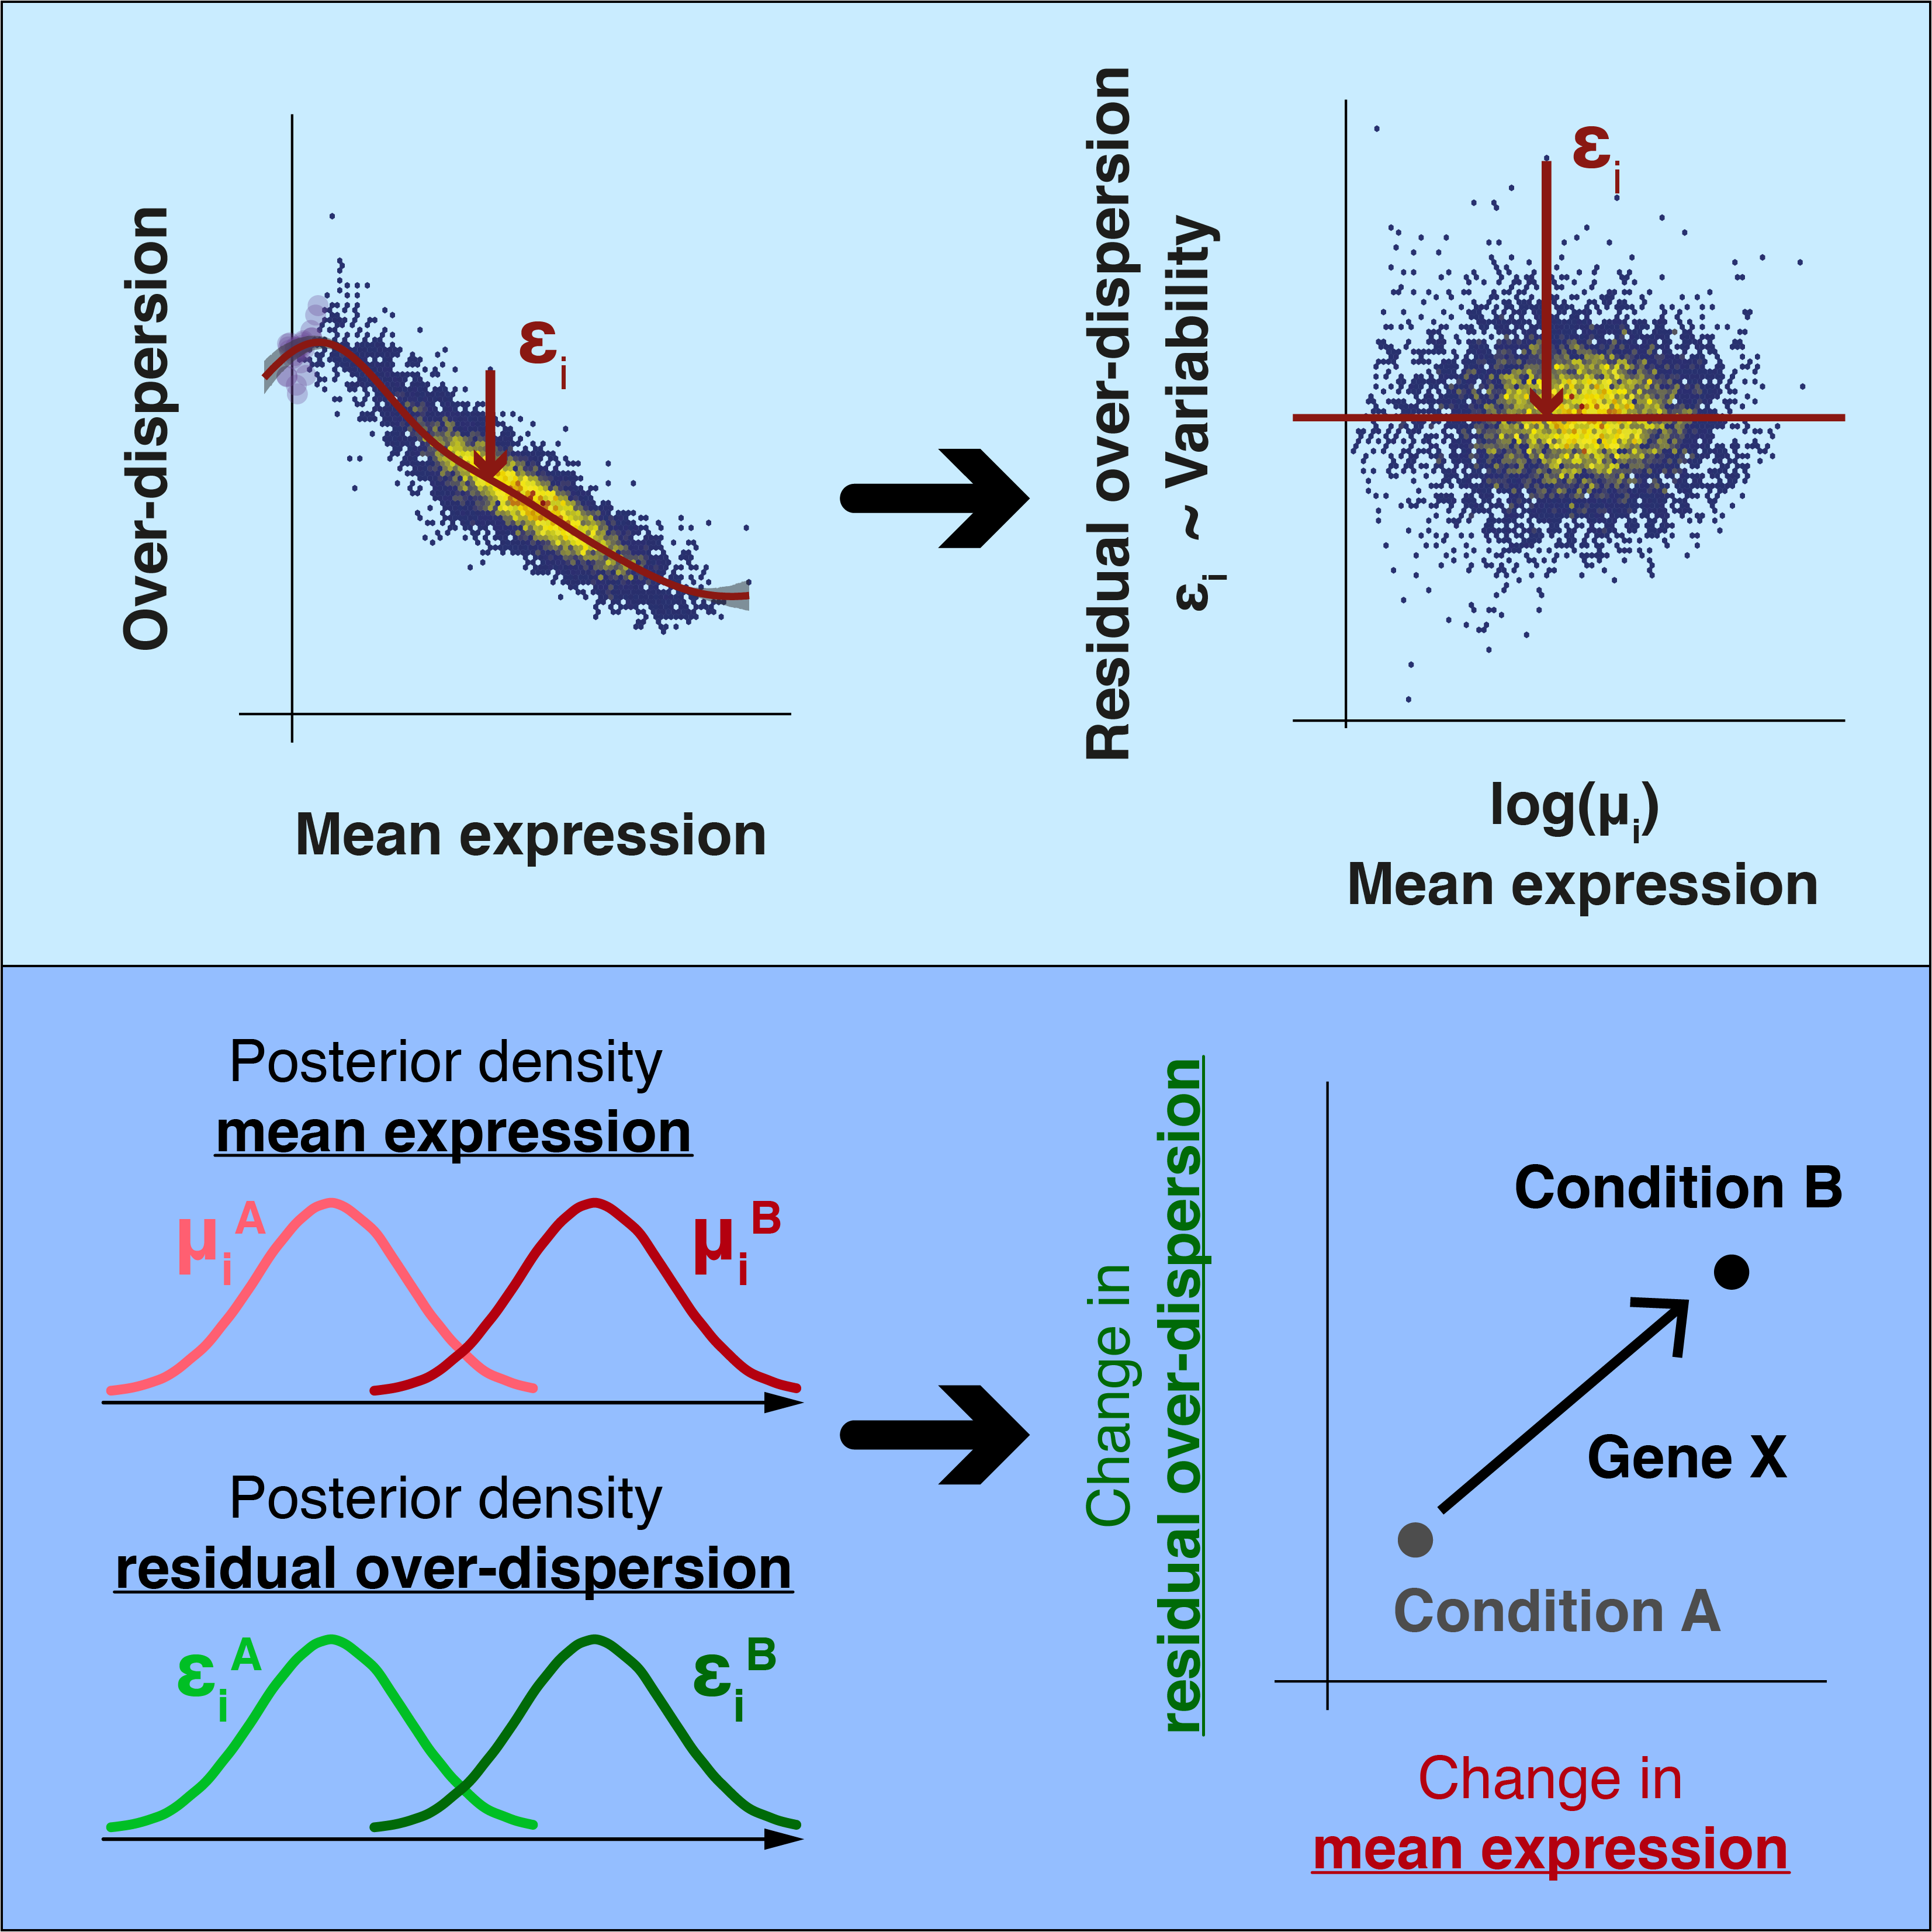
\includegraphics[width=\textwidth]{GraphicalAbstract.png}
\caption*{}
\end{figure}

\vspace*{\fill}


\newpage

% Include different main sections of the third chapter
%!TEX root = ../chapter3.tex
%******************************
%	 Introduction 
%*****************************

\section{Introduction}

Gametogenesis is the process which forms haploid gametes that carry one copy of the individuals DNA. Sexual reproduction requires the fusion of two gametes from the opposite sex to drive evolution and adaptation \citep{McDonald2016}. Spermatogenesis, the male version of gametogenesis, is a tightly regulated developmental process to generate mature sperm. 
During spermatogenesis, spermatogonial stem cells undergo a unidirectional differentiation programme to form mature spermatozoa. This process occurs in the epithelium of seminiferous tubules in the testis \textbf{(Fig.~\ref{fig3:cell_staging}B)} and is tightly coordinated to ensure the continuous production of mature sperm cells. In the mouse, the first step involves spermatogonial differentiation to form pre-leptotene spermatocytes \citep{Oakberg1971, DeRooij1973, DeRooij2000}. Pre-leptotene spermatocytes then commit to meiosis, a cell division programme that consists of two consecutive cell divisions to produce haploid cells. To accommodate homologous recombination between sister chromatids and chromosome synapsis \citep{Marston2004}, prophase of meiosis I is extremely prolonged, lasting several days in males. It can be divided into four substages: leptonema (L), zygonema (Z), pachynema (P) and diplonema (D). Following the two consecutive cell divisions, haploid cells known as round spermatids (RS) undergo a complex differentiation programme called spermiogenesis to form mature spermatozoa \citep{Oakberg1956}. \\

Spermatogenesis takes place in a highly orchestrated fashion, with tubules periodically cycling through twelve epithelial stages defined by the combination of germ cells present (see \textbf{Fig.~\ref{fig3:cell_staging}B} and \citep{Oakberg1956}). The completion of one cycle takes 8.6 days in the mouse, and the overall differentiation process from spermatogonia to mature spermatozoa requires approximately 35 days \citep{Oakberg1956a}. Thus, four to five generations of germ cells are present within a tubule at any given time. In adult animals, each tubule resides in a different cycle stage meaning that at any given time-point, the continuum of germ cell types is present in the testis \textbf{(Fig.~\ref{fig3:cell_staging})}. The continuity of this differentiation process and the gradual transitions between spermatogenic cell types have made the isolation and thus the molecular characterisation of individual sub-stages during spermatogenesis difficult.

\newpage

\begin{figure}[!h]
\centering
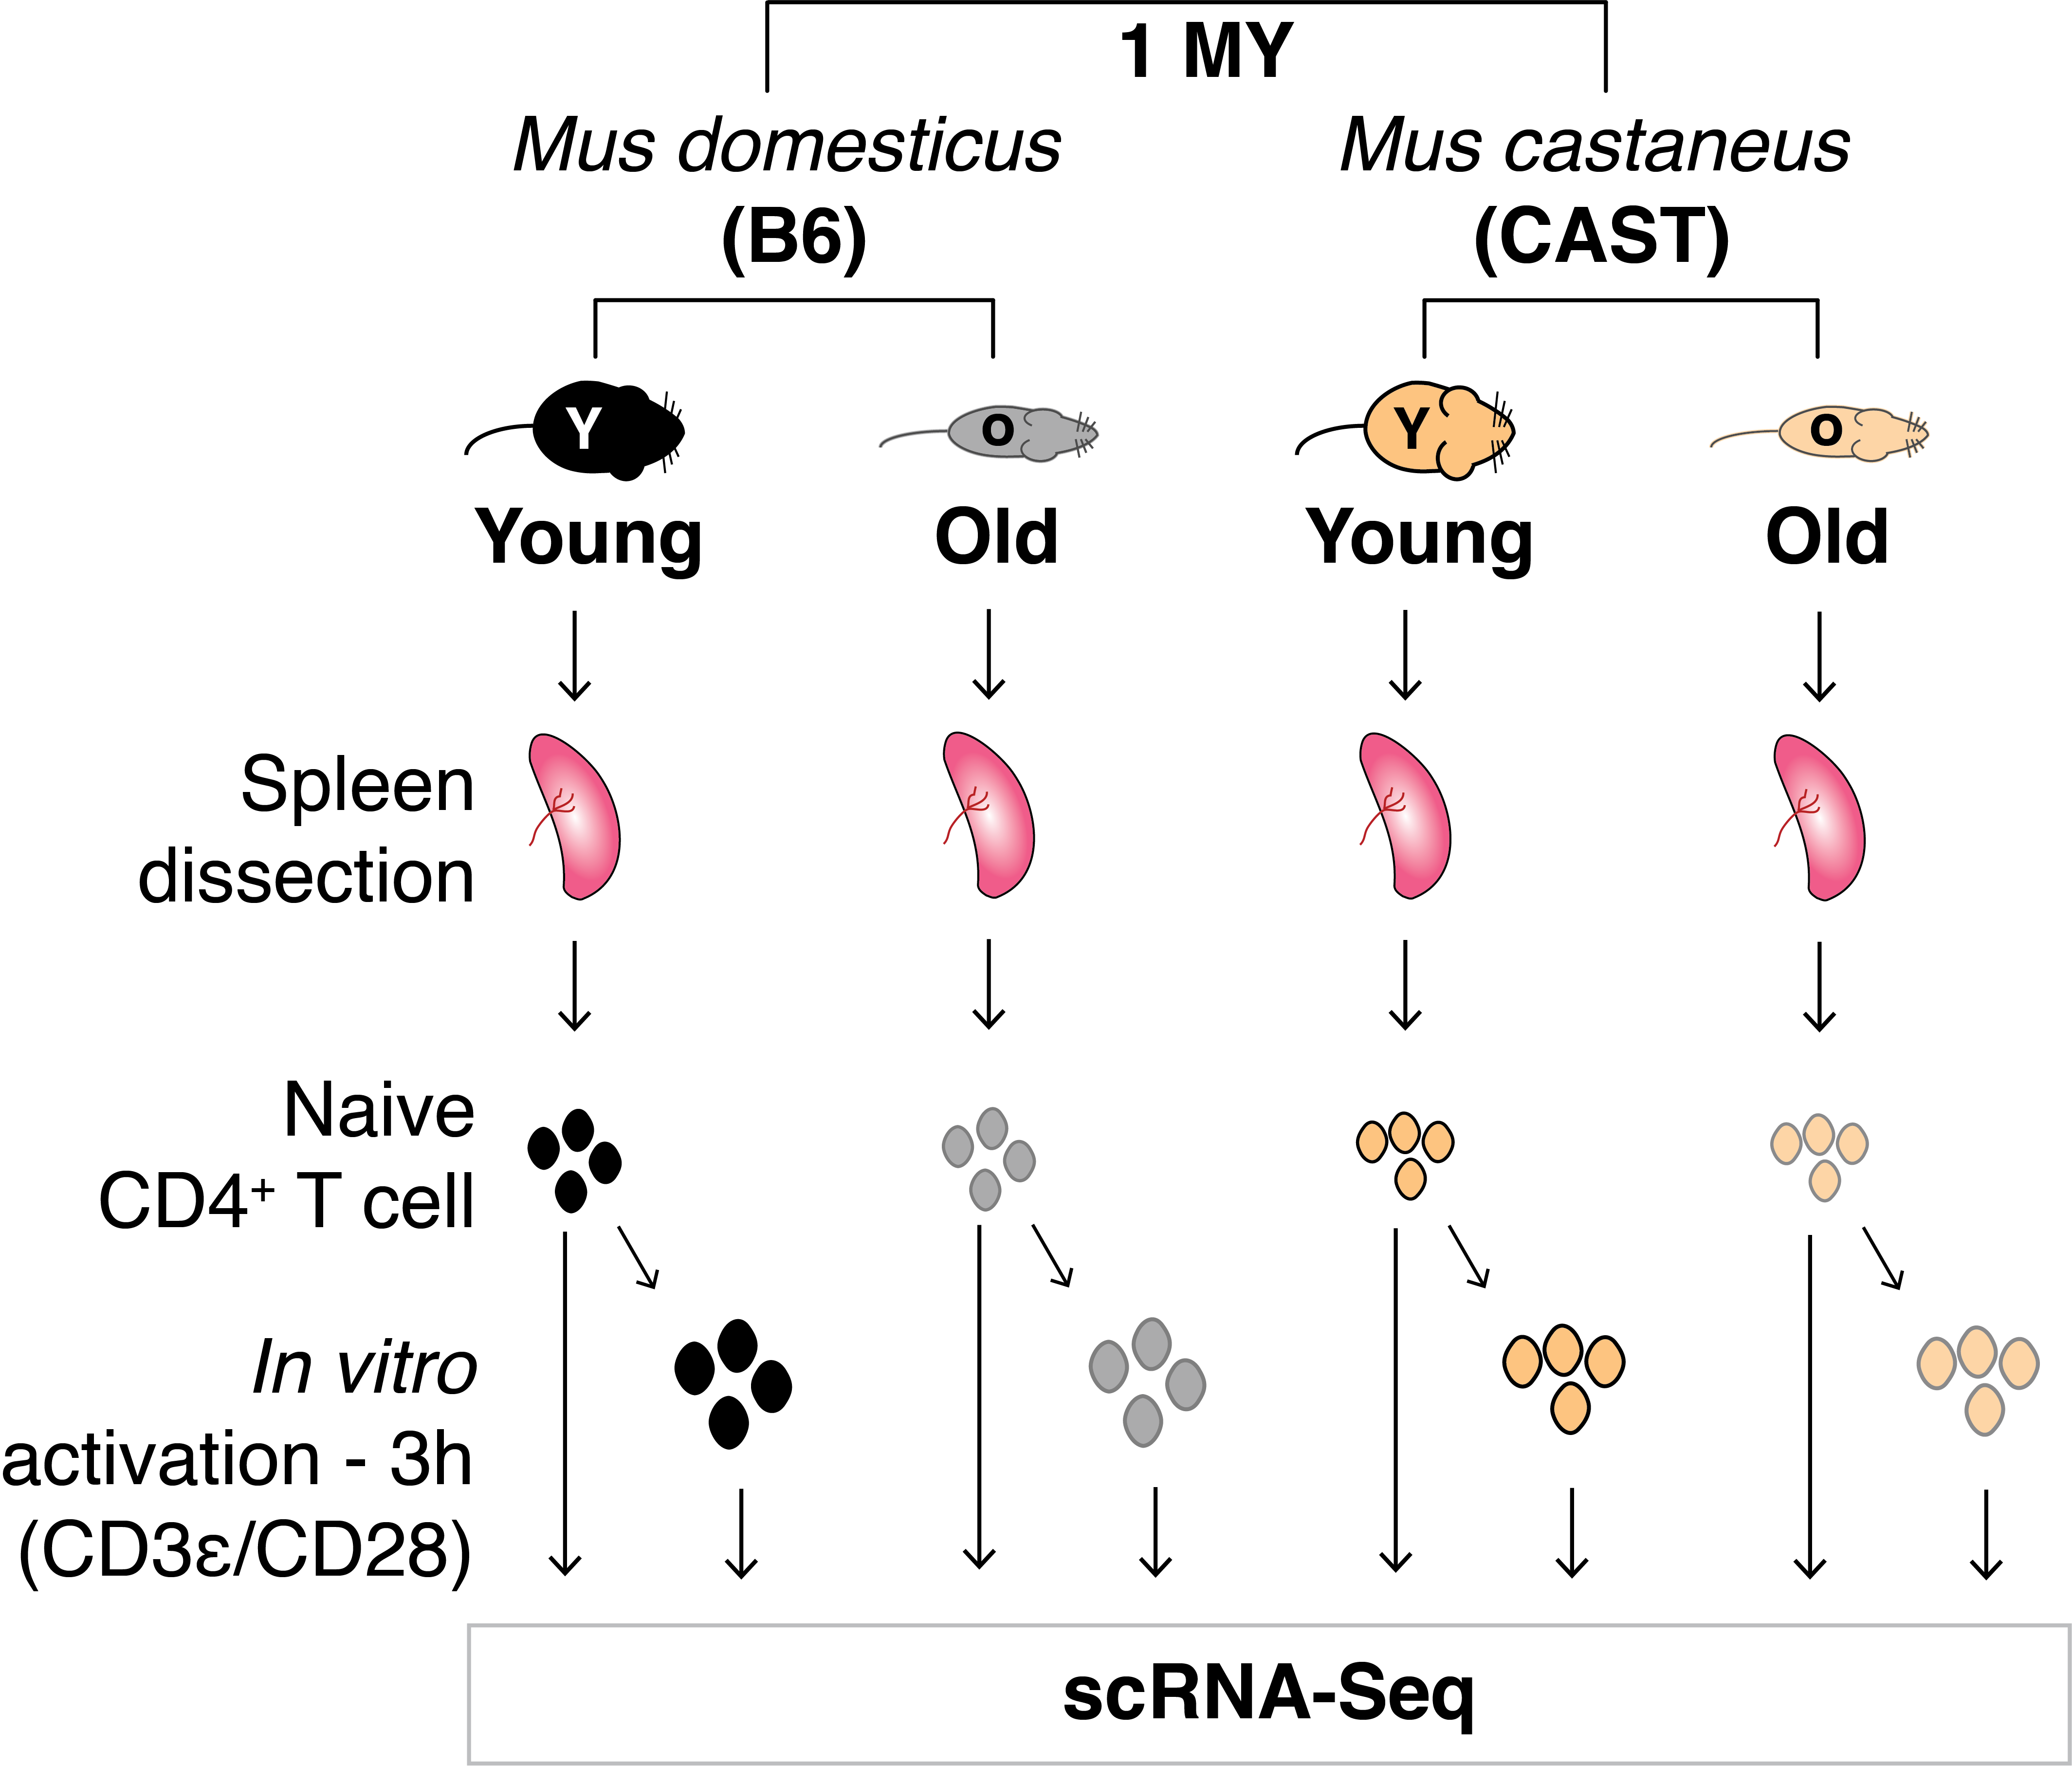
\includegraphics[width=\textwidth]{Fig_1.png}
\caption[Staging of the testicular seminiferous epithelium]{\textbf{Staging of the testicular seminiferous epithelium.}\\
\textbf{(A)} Periodic Acid Schiff (PAS)-stained testis cross-section showing a number of seminiferous tubules at different epithelial stages (displayed as Roman numerals). Within each tubule, the inset circle refers to the corresponding section in (B). Scale bar represents 100 \textmu{}m, \textbf{(B)} Schematic representation of the 12 stages of the seminiferous epithelium in mice. The colour gradient within the circle indicates the differentiation path of germ cells with the layers corresponding to individual cycles of the epithelium. The circle is divided into 12 section, each corresponding to one epithelial stage displaying the characteristic germ cells. Within each section, cells are positioned across the different layers according to their emergence during consecutive cycles, each being 8.6 days apart with more mature cells moving towards the centre, \textbf{(C)} Higher magnification of two tubules depicted in (A). The PAS-stained cross-sections show tubules in Stage VII and Stage X, with the different cell layers indicated by coloured lines. Stage VII tubules contain 4 different layers with germ cells from different generations that are approximately 8.6 days apart, whereas Stage X tubules only contain three layers. Cell types are labelled as: A – type A spermatogonia (SG), In – intermediate SG, B – type B SG, Pl – preleptotene spermatocytes (SCs), L – leptotene SCs, Z – zygotene SCs, P – pachytene SCs, D – diplotene SCs, M – metaphase I and II, 1-8 round spermatids (1-8), 9-16 elongating spermatids (9-16).}
\label{fig3:cell_staging}
\end{figure}

\newpage

To fully elucidate the molecular genetics of germ cell development, it is crucial to sample the full spectrum of germ cells present in testes of adult animals. For this purpose, we employed an unbiased droplet-based scRNA-Seq approach using the 10X Genomics\texttrademark{} platform. 
We used the transcriptomic profiles of thousands of single germ cells to characterize the complex transcriptional dynamics of spermatogenesis at high-resolution. To confidently identify and label cell populations throughout the developmental trajectory, we profiled cells from juvenile testes during the first wave of spermatogenesis. In juveniles, spermatogenesis has only progressed to a defined developmental stage, and therefore allowed us to unambiguously identify the most mature cell type by comparison with adult. The correct labelling of cell types was then used to dissect differentiation processes such as meiosis and spermiogenesis. Furthermore, juvenile samples enriched for spermatogonia which allowed us to characterize spermatogonial differentiation. Another major developmental process during spermatogenesis is the inactivation and reactivation of the X chromosome, which is subject to transcriptional silencing as a consequence of asynapsis \citep{Turner2007}. By combining bulk and single-cell RNA-Seq approaches with chromatin profiling, we identified that \textit{de novo} activated X-linked genes carry distinct chromatin signatures with high levels of repressive H3K9me3 in spermatocytes. \\

Finally, after fully characterising the transcriptional changes during spermatogenesis, I used the regression model presented in the previous chapter to study changes in transcriptional variability over the differentiation time-course. To this end, I generated \emph{post hoc} posterior distribution of linear regression coefficients to statistically test whether individual genes increase or decrease in variability. Furthermore, the clustering of variability profiles showed that rapid transcriptional changes during differentiation can cause peaks in such variability profiles.

\newpage
%!TEX root = ../chapter3.tex
%******************************
%	 Results 
%*****************************

\section{Data generation and processing strategies}

To fully dissect mouse spermatogenesis, we performed three sets of experiments: 1. droplet-based scRNA-Seq of juvenile and adult animals, 2. bulk RNA-Seq of multiple time-points during the first wave of spermatogenesis and 3. CUT\&{}RUN to profile chromatin marks in juvenile mice. The following section will give an overview on the data generation and processing approaches. Detailed analysis steps are explained throughout the chapter. The full experimental set-up can be seen in \textbf{Fig.~\ref{fig3:experimental_design}}.

\begin{figure}[!h]
\centering
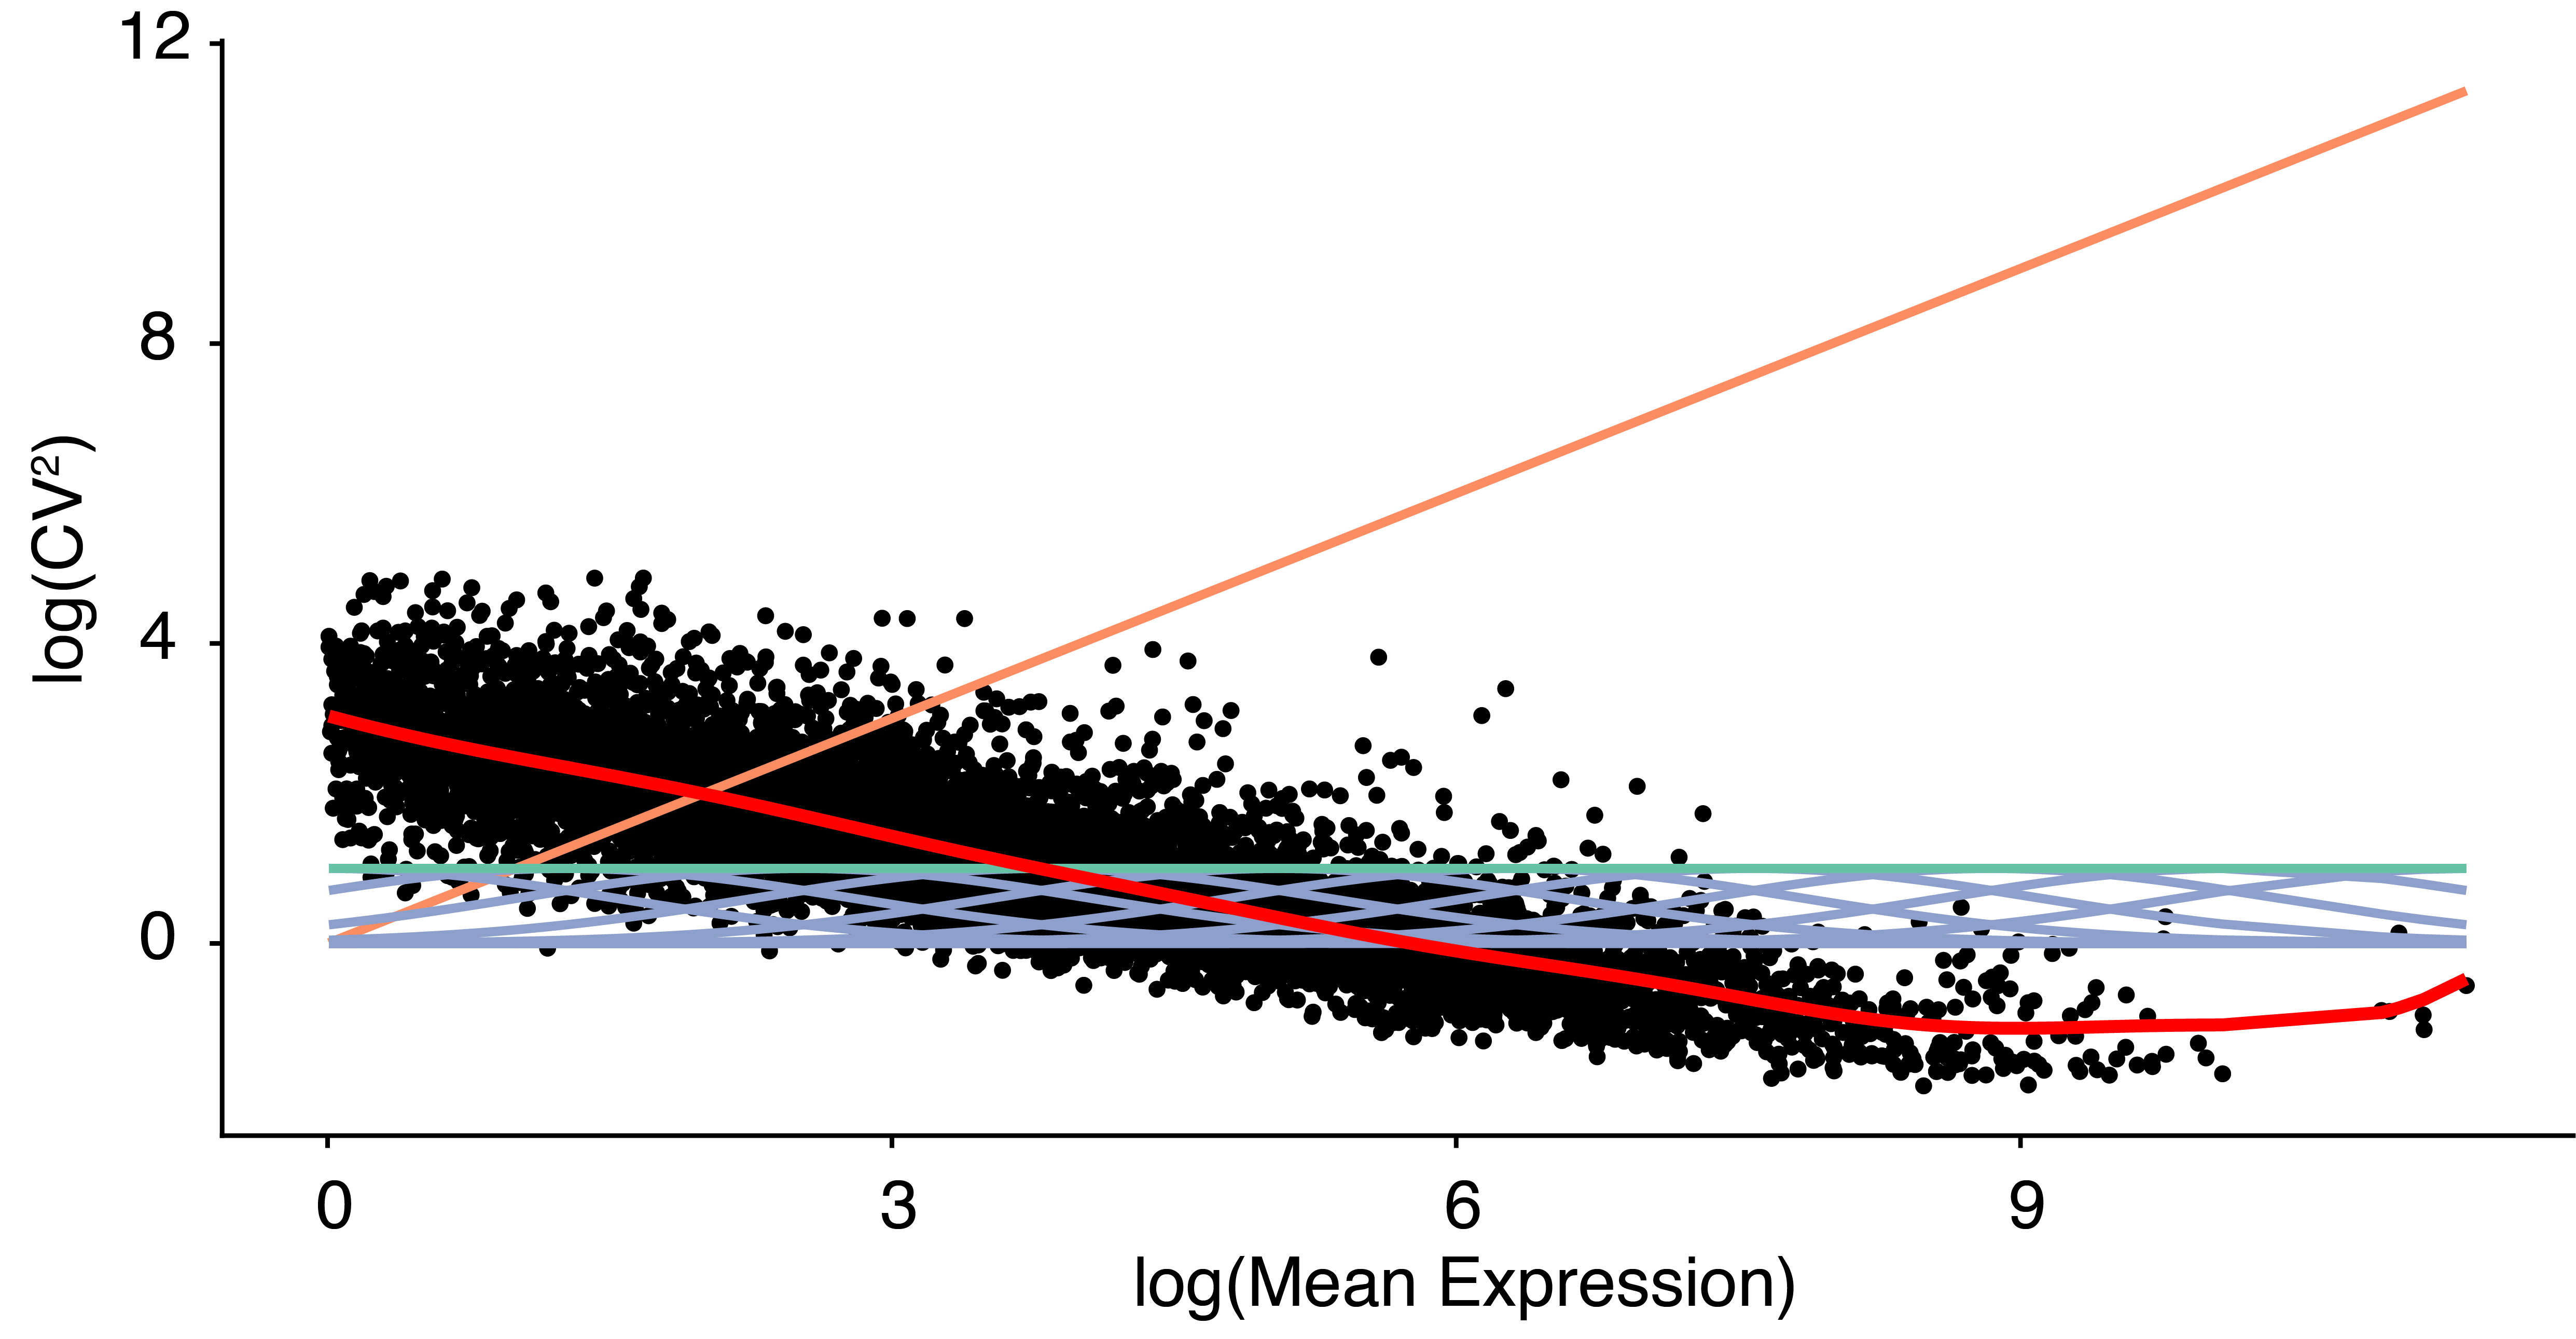
\includegraphics[width=\textwidth]{Fig_2.png}
\caption[Experimental design to dissect mouse spermatogenesis]{\textbf{Experimental design to dissect mouse spermatogenesis.}\\
Overview of the experimental design yielding bulk RNA-Seq, droplet-based scRNA-Seq and chromatin profiling on FACS-purified cells using CUT\&{}RUN from one testis while using the contralateral testis for matched histology.}
\label{fig3:experimental_design}
\end{figure}

\subsection{scRNA-Seq using the 10X Genomics\texttrademark{} system}

Droplet based single-cell RNA sequencing was performed using the 10X Genomics\texttrademark{} technology \citep{Zheng2017}. For this, testes from specifically staged juvenile (between postnatal days 6 and 35) and adult (8-9 weeks) C57BL/6J (B6) mice were dissociated. Single-cell suspensions were loaded into one channel of the 10X Chromium\texttrademark{} Single Cell A Chip, aiming for a recovery of 4000-5000 high-quality cells. Further information on the experimental strategy can be found in \textbf{Appendix \ref{appA.2}} and \textbf{Table \ref{tab3:QC_scRNAseq}} summarises the cells captured per sample.

\newpage

\begin{table}[ht	]
\centering
\caption[Quality filtering of scRNA-Seq data]{\textbf{Quality filtering of scRNA-Seq data.} \\
Quality metrics of droplet-based scRNA-Seq. \textbf{Sample:} Stage information for all samples, \textbf{Library:} sample identifier, \textbf{CellRanger filter:} Number of retained cells after default thresholding using the CellRanger \emph{counts} function,  \textbf{After QC:} Number of cells obtained after quality control (QC), \textbf{Assigned Cell Type:} Number of cells that fall into annotated clusters (removing outlying cells), \textbf{EmptyDrops filter:} Number of cells retained after using the \emph{emptyDrops} function controlling the FDR to 1\%, \textbf{EmptyDrops QC:} Number of cells obtained after quality control (QC) of the \emph{emptyDrops} filtered cells.}
\label{tab3:QC_scRNAseq}
\begin{tabular}{lllllll}
\toprule
\textbf{Sample} & \textbf{Library} & \textbf{CellRanger} & \textbf{After} & \textbf{Assigned} & \textbf{EmptyDrops} & \textbf{EmptyDrops} \\
& & \textbf{filter} & \textbf{QC} & \textbf{Cell Type} & \textbf{filter} & \textbf{QC} \\
\midrule
Adult & do17815 & 1157 & 1157 & 1123 & 4467 & 3400 \\
\midrule
Adult & do17816 & 2198 & 2198 & 2092 & 6145 & 4603 \\
\midrule
P10 & do17821 & 3229 & 3213 & 3212 & 4976 & 4202 \\
\midrule
P15 & do18195 & 4258 & 4258 & 4014 & 14050 & 13168 \\
\midrule
P20 & do17824 & 1775 & 1775 & 1662 & 9400 & 7491 \\
\midrule
P25 & do18196 & 4334 & 4334 & 4130 & 8038 & 6802 \\
\midrule
P30 & do17825 & 2278 & 2278 & 2211 & 5393 & 4958 \\
\midrule
P35 & do17827 & 3160 & 3160 & 3004 & 49002 & 10683 \\                 
\bottomrule   
\end{tabular}
\end{table}

To process droplet-based scRNA-Seq data after sequencing, 10X genomics\texttrademark{} developed a set of processing pipelines termed \textit{Cell Ranger}. We obtained gene-specific transcript counts using the Cell Ranger \emph{count} function with default settings. This pipeline aligns reads against the \emph{Mus musculus} genome (GRCm38) and counts UMIs per transcript and sample. This software retains cells with similar UMI distributions \citep{Zheng2017}. We use this default threshold to obtain high-quality cells with large numbers of UMIs. For further quality control and after merging cells of all samples, we filtered out cells that express less than 1000 genes. Additionally, we exclude cells with more than 10\% of reads mapping to the mitochondrial genome. The number of remaining cells per sample can be seen in \textbf{Table \ref{tab3:QC_scRNAseq}}.\\

The Cell Ranger \emph{count} pipeline performs thresholding on the number of UMIs per cell to exclude empty droplets or droplets with low-quality cells. This default threshold excludes smaller cells with lower transcriptional complexity form a mixture containing cells with broadly different transcriptional complexities. We therefore used the \emph{emptyDrops} function provided in the \emph{DropletUtils} Bioconductor package to statistically distinguish empty droplets from genuine cells (controlling the FDR to 1\%) \citep{Lun2018}. Nevertheless, further quality control needs to be performed and after merging all remaining cells across all samples, we filtered out cells with less than 500 genes expressed. Furthermore, we excluded cells with more than 10\% or mitochondrial genes expressed \textbf{(Table \ref{tab3:QC_scRNAseq})}.\\
 
The transcriptomes of quality filtered cells were normalized using the \emph{scran} package \citep{Lun2016pooling}. For this, cells with similar transcriptomic complexity were pre-clustered using a graph-based approach (as implemented in the \emph{quickCluster} function). Size factors were
calculated within each cluster before being scaled between clusters using the \emph{computeSumFactors} function. Throughout this paper, the log$_2$-transformed, normalized counts (after adding one pseudocount) are displayed. For down-stream analysis, lowly expressed genes (averaged log$_2$-transformed, normalized expression < 0.1) were excluded. After quality control and filtering, we retained more than 20,000 high-quality single cells and over 46,000 cells including the once with lower transcriptional complexity \textbf{(Table \ref{tab3:QC_scRNAseq})}. These cells were used to dissect molecular processes during spermatogenesis and to profile under-represented and transcriptionally inactive cell types in mouse testes. 

\subsection{Bulk RNA-Seg from juvenile animals}

Additionally, we generated whole-tissue bulk RNA-Seq libraries from time-points during the first wave of spermatogenesis (\textbf{Appendix \ref{appA.2.bulk}}). More specifically, we sampled (in replicates) testes from mice at post-natal (P) day P6 (2x), P8, P10 (2x), P12 (2x), P14 (2x), P16, P18 (2x), P20 (2x), P22 (2x), P24 (2x), P26 (2x), P28 (2x), P30 (2x), P32, P34, P35 and from adult animals (2x). Detailed experimental methods can be found in \textbf{Appendix \ref{appA.2.bulk}}. 
Sequencing reads were aligned against the \textit{Mus musculus} genome (GRCm38) using the \emph{STAR} aligner with default settings \citep{Dobin2013}. \\

Gene-level transcript counts were obtained using \emph{HTSeq} \citep{Anders2014} with the –s option set to “reverse” and using the GRCm38.88 genomic annotation file. We visualized several features of the aligned and counted data (number of intronic/exonic reads, number of multi-mapping reads, low-quality reads and total library size) and did not detect any low-quality RNA-Seq libraries. Next, we used the size factor normalization approach implemented in DESeq2 \citep{Love2014} for data normalization. For down-stream analysis and visualization, lowly expressed genes (averaged counts < 10) were excluded. With this, we generated 30 bulk RNA-Seq libraries that will be used for developmental staging of cell types and the dissect X chromosome expression dynamics.

\subsection{CUT\&{}RUN from juvenile animals}

To map chromatin states in purified cell populations we used CUT\&{}RUN (Cleavage Under Targets \& Release Using Nuclease) \citep{Skene2018}. Detailed experimental methods can be found in \textbf{Appendix \ref{appA.2.CnR}}. In brief, spermatocytes and spermatids were sorted as described in \textbf{Appendix \ref{appA.2.sorting}} and attached to concanavalin A–coated magnetic beads. After permeabilisation, anti-bodies against H3K9me3 and H3K4me3 were incubated with the cells. Inactive micrococcal nuclease linked to protein A was added to the mix and cooled to 0$^\circ$. Protein A binds to the antibodies and upon activation the nuclease digests DNA next to the histones where the antibody bound. Cleaved DNA fragments diffused out of the nucleus and were prepared for sequencing. This technique allows targeted chromatin profiling for specific marks at a genome wide level and requires minimal cell input \citep{Skene2018}.\\

Sequencing reads were aligned to the Mus musculus genome (GRCm38) using \textit{Bowtie2} with the following settings: --local --very-sensitive-local --no-unal -q --phred33. Paired end reads were counted in specified regions using the \textit{regionCounts} function implemented in the \textit{csaw} Bioconductor package \citep{Lun2015}. For this, duplicated reads, reads mapped more than 1000 bp apart and reads mapping to blacklisted regions (available at: \url{http://mitra.stanford.edu/kundaje/akundaje/release/blacklists/mm10-mouse/mm10.blacklist.bed.gz}) were removed. Regions of interests were: promoters (obtained using the \textit{promoters} function of the \textit{GenomicFeatures} package), 1000 bp windows across the chromosome (using the \textit{windowCounts} function of \textit{csaw}) and whole chromosomes. Counts per region were normalized based on library size (counts per million, CPM) for promoter regions and 1000 bp windows. Additionally, when considering entire chromosomes, the length of the chromosome was accounted for by computing the Fragments per Kilobase per Million mapped reads (FPKMs). 

\newpage

\subsection{Identification of germ cell-types across all scRNA-Seq samples}
\label{sec3:clustering}

After data generation and pre-processing steps, we next characterized the detectable cell-types across all scRNA-Seq samples. We assume that cell-types sampled from juvenile animals are also found among the cell types sampled from adult animals. To detect cell-types consistently across all scRNA-Seq samples, we first performed batch correction. To remove batch-specific effects that arise when samples are prepared and sequenced in different experiments \textbf{(Tables \ref{tab3:QC_scRNAseq})}, we used the \emph{mnnCorrect} function implemented in the \emph{scran} package \citep{Haghverdi2018}. We used the top 1000 genes with highest biological variation across all samples as informative genes for batch correction. The \emph{mnnCorrect} function takes transcriptional profiles of cells isolated from adult B6 mice as first input and uses this dataset as reference for cell mapping. This approach maps the juvenile samples onto the adult B6 \textbf{(Fig.~\ref{fig3:cell_types}A)}.\\

To identify cell types across all samples, batch corrected transcriptomes were clustered using a graph-based approach. A shared nearest-neighbour (SNN) graph \citep{Xu2015} was constructed considering 3 shared nearest neighbours using the \emph{buildSNNGraph} function in \emph{scran}. In the next step, a multi-level modularity optimization algorithm was used to find community structure in the graph \citep{Blondel2008} implemented in \emph{igraph} R package. Cells in small clusters that show unclear identities were excluded from down-stream analysis. In total, we identified 28 cluster. To correctly label cell clusters based on their cell-type, we identified marker genes for all germ cell-types in the adult B6 samples. To this end, we performed differential expression testing using multiple pairwise comparisons. To detect cluster-specific marker genes, the \emph{findMarkers} function implemented in \emph{scran} was used on the log$_2$-transformed normalized counts while providing the cluster labels \textbf{(Fig.~\ref{fig3:cell_types}B)}. \\

On a broad level and by visualizing the expression of detected marker genes, we identified the following cell types: spermatogonia (based on \textit{Dmrt1} expression, \citep{Matson2010}), spermatocytes (\textit{Piwil1}, \citep{Deng2002}), round and elongating spermatids (\textit{Tex21} and \textit{Tnp1}, respectively, \citep{Fujii2002}), as well as the main somatic cell types of the testis, Sertoli (\textit{Cldn11}, \citep{Mazaud-Guittot2010}) and Leydig cells (\textit{Fabp3}, \citep{Oresti2013}) \textbf{(Fig.~\ref{fig3:cell_types}B)}. Using a dimensionality reduction technique for visualization (t-distributed Stochastic Neighbour Embedding; \textbf{Fig.~\ref{fig3:cell_types}C}), the germ cell types from spermatocytes to elongating spermatids formed a continuum, which recapitulated the known developmental trajectory.

\newpage

\begin{figure}[!h]
\centering
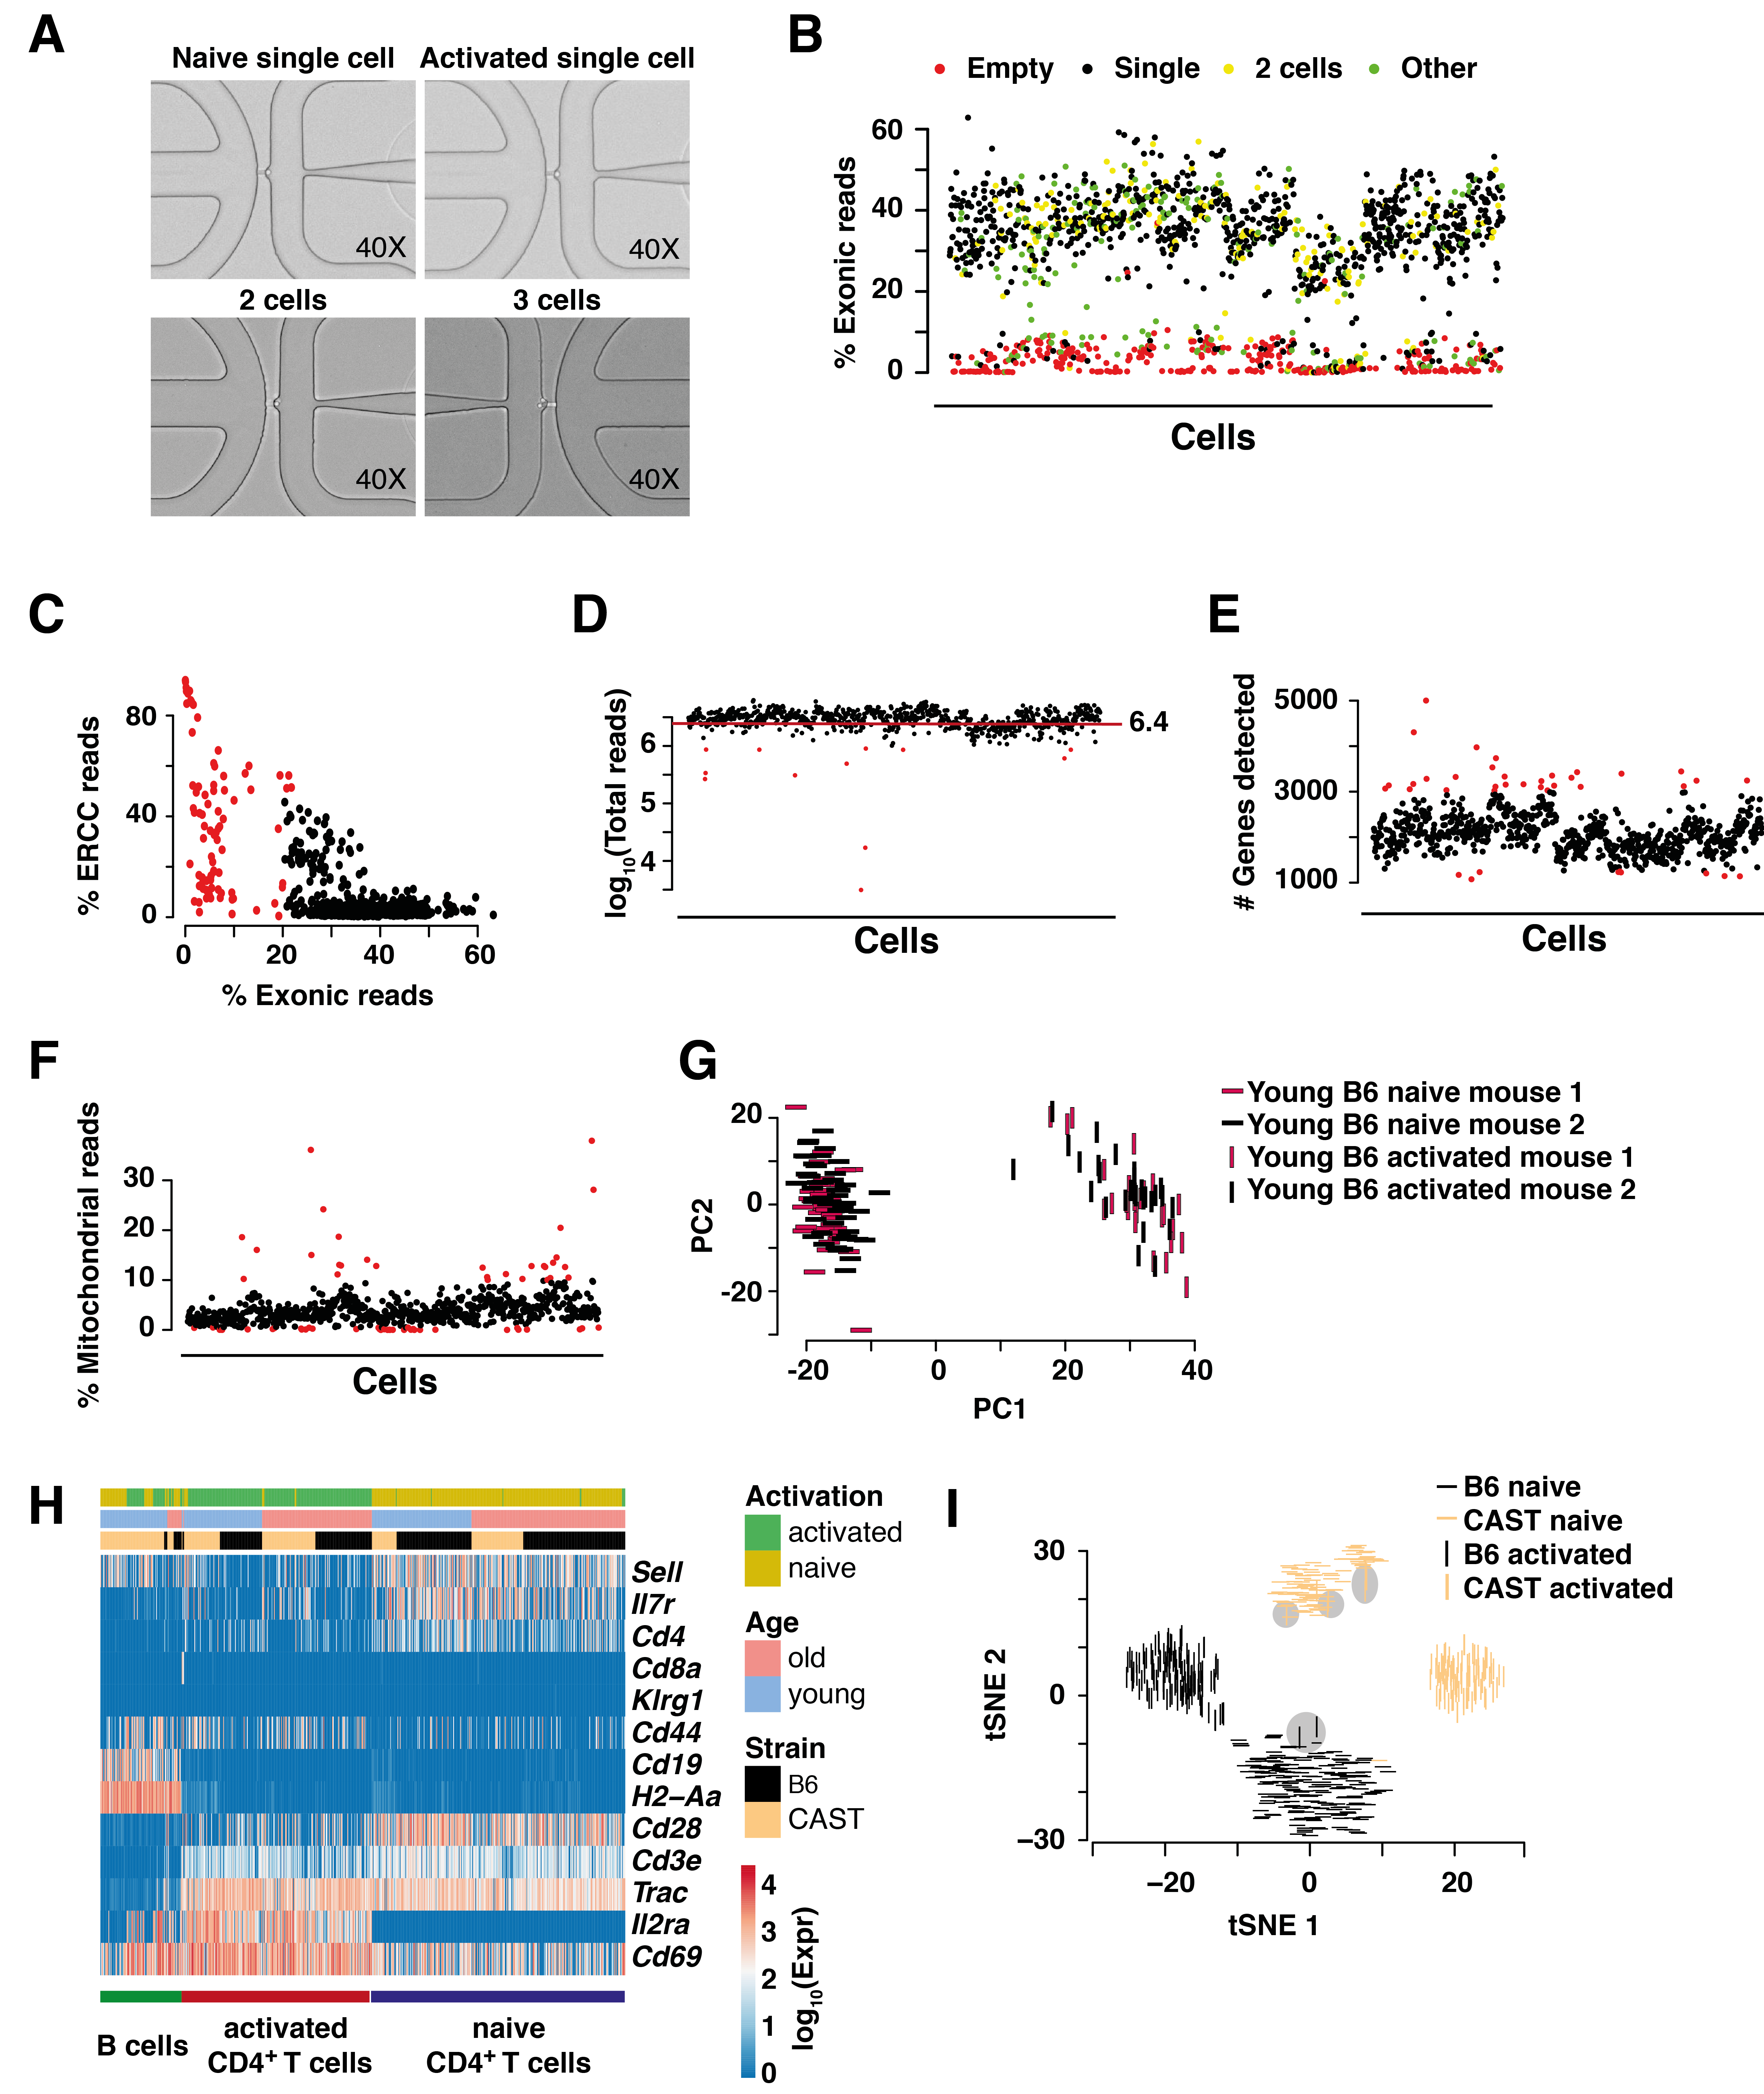
\includegraphics[width=\textwidth]{Fig_3.png}
\caption[Droplet based scRNA-Seq of juvenile and adult mouse spermatogenesis]{\textbf{Droplet based scRNA-Seq of juvenile and adult mouse spermatogenesis.}\\
\textbf{(A)} tSNE representation of juvenile cells that were mapped to cells isolated from adult mice. Grey dots indicate all cells from adult animals that were used as a reference for cell mapping. Coloured dots represent cells isolated at each sampled stage during the first wave of spermatogenesis. Clustering has been perfomed across all cells after cell mapping. SG: Spermatogonia, M: Metaphase, IL: Imature Leydig, PTM: Peritubular Myoid Cells, EC: Endothelial Cells, tMg: testicular Marcophages, \textbf{(B)} tSNE representation of scRNA-Seq data from adult B6 mice with the colour gradient representing the expression of known marker genes for two somatic cell types and the main germ cell types. The x- and y-axis represent the first and second dimension of tSNE respectively. The colour legend shows log$_2$-transformed, normalized expression counts, \textbf{(C)} Graph-based clustering identifies different sub-stages within major germ cell populations form adult B6 animals. 
}
\label{fig3:cell_types}
\end{figure}

\newpage

\section{Developmental staging of mouse spermatogenesis}

Historically, sub-staging of the major cell types within the testis was based on changes in nuclear or cellular morphology \citep{Oakberg1956,  Oakberg1956a}. Previous attempts to complement morphology with molecular signatures have been limited to FACS-based and sedimentation assays, where the resolution was unable to differentiate between sub-cell-types \citep{Bastos2005, Gaysinskaya2014, Lam1970, Meistrich1977, Romrell1976, Soumillon2013}. While a mixture of all spermatogenic cell types co-exists in the adult, the first wave of spermatogenesis during juvenile development is more synchronised. Starting around mouse postnatal day P4, spermatogonia begin to differentiate, forming the first generation of spermatocytes as early as P10, round spermatids by P20, and completing the first wave of spermatogenesis with the production of mature spermatozoa between P30 and P35 \textbf{(Fig.~\ref{fig3:cell_staging}B and \ref{fig3:1st_wave}A)} \citep{Bellve1977, Janca1986, Nebel1961}. In this section, we define well-known developmental transitions during spermatogenesis by (i) mapping cells sampled from defined epithelial stages during the first wave of spermatogenesis to cells sampled from adult testes and (ii) classifying the cell-types identified above using bulk RNA-Seq sampled from juvenile testes every two days during the first wave of spermatogenesis. 

\subsection{Cell type characterization using the first wave of spermatogenesis}
 
We exploited the synchronised development of cell types throughout the first wave of spermatogenesis to define major and morphologically described check-points of the differentiation process. For this, we sampled multiple time-points from juvenile animals to identify the most mature (differentiated) cell types. At any given time-point during the first wave of spermatogenesis, there exist a defined number of known cell types in juvenile testis depending on the timing of the developmental cycle \textbf{(Fig.~\ref{fig3:cell_staging}B)}. Based on known sperm developmental transitions, we chose six time points between P10 and P35 from which to generate single-cell RNA-Seq libraries \textbf{(Fig.~\ref{fig3:1st_wave}A and Table \ref{tab3:QC_scRNAseq})}. As described above, we mapped the transcriptomes of juvenile samples onto the adult B6 sample \textbf{(Fig.~\ref{fig3:cell_types}A)}. For each juvenile experiment, we found that the population of developing germ cells was strongly enriched at the expected developmental stage, as quantified by the percentage of cells in each cell-type cluster \textbf{(Fig.~\ref{fig3:1st_wave}C)}. By associating the known cell-types from juvenile animals with the corresponding cell types in the adult trajectory, we unambiguously assigned molecular and histological signatures to cells during adult spermatogenesis.

\newpage

\begin{figure}[!h]
\centering
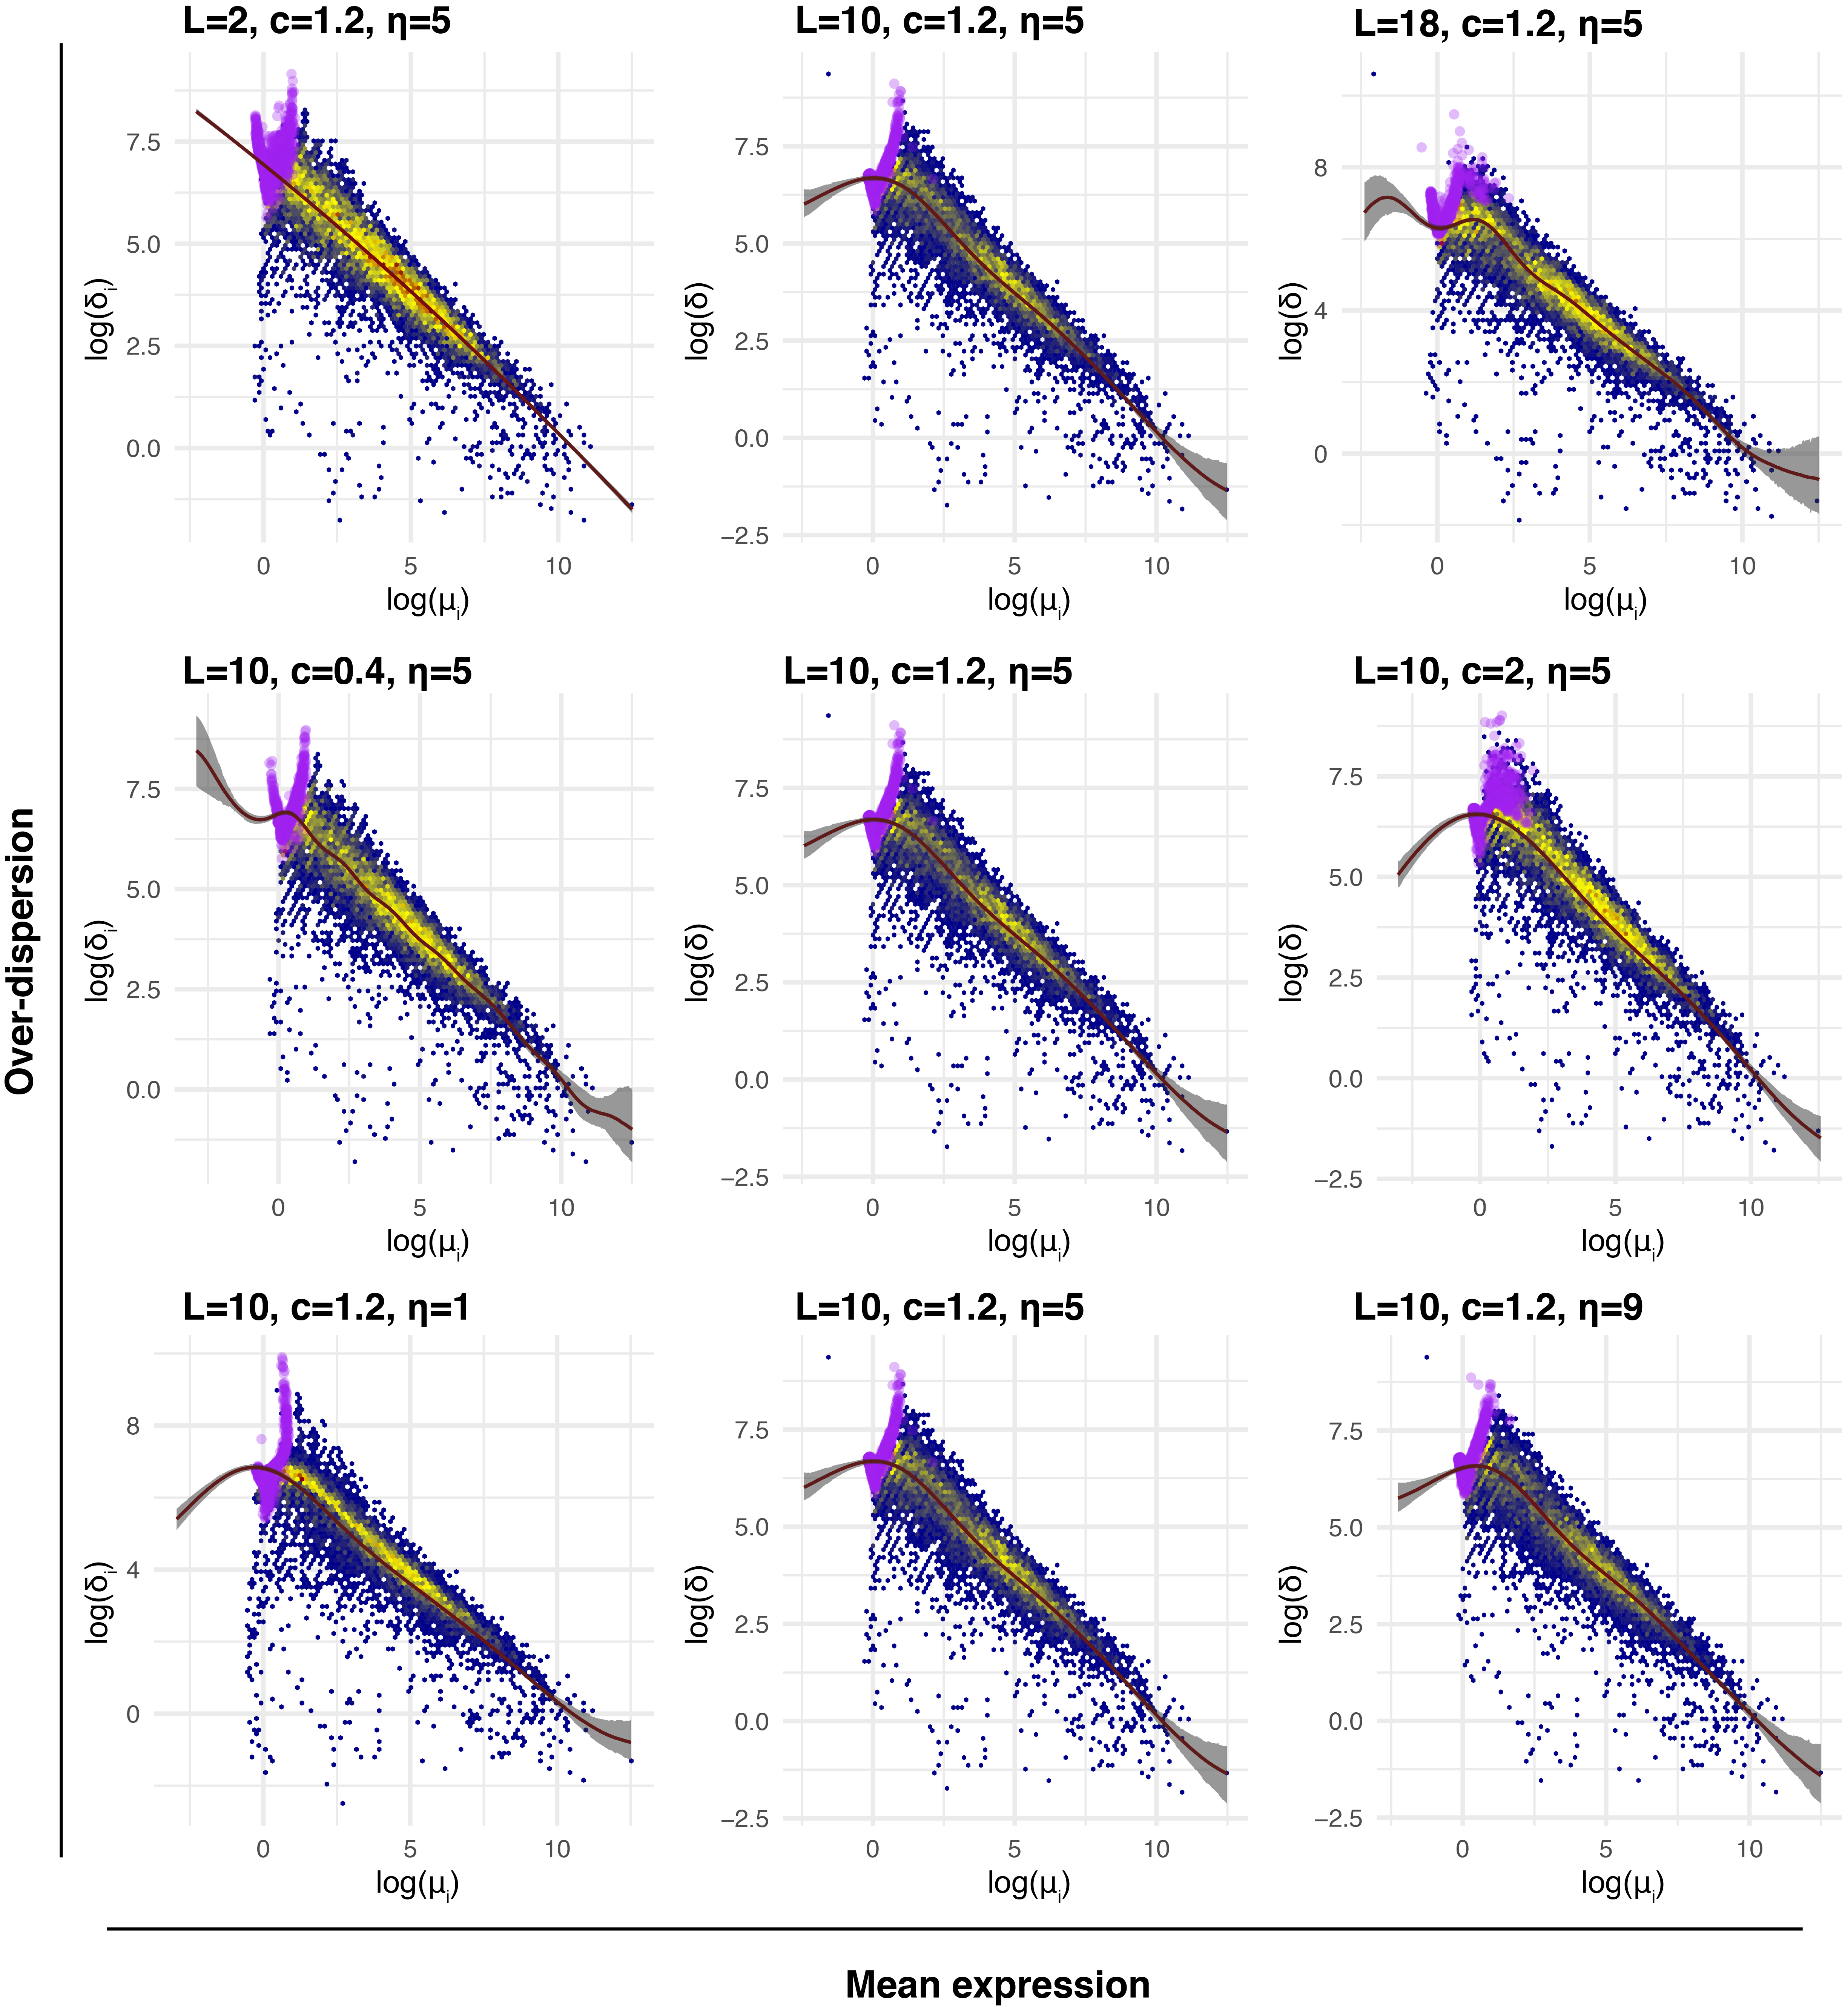
\includegraphics[width=0.95\textwidth]{Fig_4.png}
\caption[Staging of cell types during mouse spermatogenesis]{\textbf{Staging of cell types during mouse spermatogenesis (full legend on next page).}}
\label{fig3:1st_wave}
\end{figure}

\newpage

\captionsetup[figure]{list=no}
\addtocounter{figure}{-1}   
\captionof{figure}{\textbf{Staging of cell types during mouse spermatogenesis (continued).}\\
\textbf{(A)} Schematic representation of the major germ cell types and their corresponding developmental processes. Spermatogonia differentiate undergoing mitotic cell divisions before forming spermatocytes that divide by meiotic division. Following meiosis, spermatids differentiate throughout spermiogenesis to form mature sperm. The timeline in the lower panel indicates at which point during the first wave of spermatogenesis samples were harvested for the generation of scRNA-Seq (X) or bulk RNA-Seq (B) data, \textbf{(B)} Representative images of seminiferous tubules from animals harvested at different postnatal (P) time points during the first wave of spermatogenesis. The approximate timing of the stage and cycle of the tubule is illustrated below in the form of a circle (see Fig.~\ref{fig3:cell_staging}B), \textbf{(C)} After cell mapping and clustering, the percentage of cells in each cluster can be calculated for each sample. The size of squares corresponds to this percentage and the colours indicate the cluster labels depicted in Fig.~\ref{fig3:cell_types}C. tSNEs on the right-hand side of each panel (juvenile samples only) illustrate progress through spermatogenesis. SG: spermatogonia, M: metaphase, \textbf{(D)} Probabilistic mapping of bulk RNA-Seq libraries to the cell clusters identified in the adult scRNA-Seq data using a random forest approach. The colour gradient indicates the probability with which a bulk sample can be assigned to the specific cell cluster.  \\}
\captionsetup[figure]{list=yes}

In adult, we detect a homogeneous distribution of cells across the germ cell types ranging from spermatogonia to S14 spermatids \textbf{(Fig.~\ref{fig3:1st_wave}C)}. To characterize germ cell-types, we focused on samples taken from P15-P35 animals since at P10 the majority of cell types do not show germ cell properties \textbf{(Fig.~\ref{fig3:cell_types}A)}. In earlier stages, cells are enriched the most mature cell-type in each cycle. For instance, at P15 the majority of cells are spermatogonia and spermatocytes progressing through the mid-pachytene stage \citep{Turner2004}. Interestingly, less mature cells-types that exists earlier to mid-pachytene cells are also present at this time point (and later time points). This supports recent reports that the first wave of spermatogenesis is less synchronized than previously anticipated \citep{Snyder2010}. At P20, we detect an enrichment for spermatocytes, cells undergoing meiotic cell division, and a small group of early round spermatids. This population structure is in line with matched histology, which shows a large number of tubules in late stages IX-XII and the first occurrence of early round spermatids \citep{Bellve1977}. It has been shown that spermatids first reach the elongating state, which occurs from S10 spermatids onwards, between P24 and P26 \citep{Janca1986}. At P25, we observed that cells mapped to our first ten clusters of spermatids, which we then labelled according to morphologically-defined spermatid substages S1 – S10 \textbf{(Fig.~\ref{fig3:1st_wave}C)}. At P30 and P35, we observed a relatively even distribution of cells across all groups, closely resembling the adult distribution up to S14, indicating that the first wave of spermatogenesis is complete. With this computational mapping of cells collected at different developmental time-points, we linked transcriptional profiles of single cells to, morphologically defined transitions during germ cell development.

\newpage

\subsection{Classification of cell types based on bulk RNA-Seq data}

While the analysis performed above only determines crucial developmental transitions during spermatogenesis, we did not achieve high-resolution for the developmental mapping of defined cell-types to the clusters identified above. To further validate the identity of the cell clusters, we used bulk RNA-Seq from testis collected during the first wave of spermatogenesis. These samples were harvested every two days between P6 and P34 and allow us to refine the mapping analysis performed above \textbf{(Fig.~\ref{fig3:1st_wave}A)}. The batch-correction approach used above was developed to match hundreds of single cells across samples and is therefore not suitable to map the 30 bulk RNA-Seq samples onto the adult trajectory. To classify each bulk RNA-Seq sample to one or multiple clusters identified in the scRNA-Seq data, we used a regression approach that performs probabilistic classification. Using the top 50 cluster-specific marker genes for spermatogonia, all spermatocyte groups, all spermatid groups, sertoli and leydig cells, we trained a random forest classifier (implemented in the \emph{randomForest} R package \citep{Liaw2002}) on 2000 cells isolated from adult B6 testes. Model testing was performed on the remaining 1215 cells isolated from adult B6 testes. Prior to training and testing, log$_2$-transformed, normalized counts were scaled by computing the Z score for each gene. Probabilistic prediction was performed using the Z score of log$_2$-transformed, normalized bulk RNA-Seq reads of the input genes. The output of this analysis is the classification probability for each bulk RNA-Seq sample to belong to each scRNA-Seq cluster.\\

This classification confirmed that between P6 – P14 spermatogonia and somatic cells show the highest contribution to the transcriptomic profile \textbf{(Fig.~\ref{fig3:1st_wave}D)}. Between P16 and P20 we observed the emergence of spermatocyte-specific gene expression signatures, after which spermatids become the transcriptionally dominant cell type. By P26, spermatids reach the elongating state where transcription is uniformly shut-down due to the beginning of the histone-to-protamine transition \citep{Steger1999}. Following this, changes in RNA content are mostly due to degradation. Bulk transcriptional profiles can only be classified up to S10 because transcription is largely inactive thereafter and no new cluster-specific marker genes emerge.  

\newpage

\section{Under-represented cell types in spermatogenesis}

The analysis of early stages of juvenile mice in the previous section showed an enrichment for cell-types that are relatively under-represented in later stages and in adult (e.g.~spermatogonia and early spermatocytes at P15, \textbf{Fig.~\ref{fig3:1st_wave}C}). Additionally, we detected the absence of germ cells in the P10 sample which leads to a relative enrichment of somatic cell types present in mouse testes \textbf{(Fig.~\ref{fig3:cell_types}A)}. This relative enrichment allows us to dissect somatic cell types and spermatogonial differentiation at higher resolution compared to cells isolated from adult samples.

\subsection{Somatic cell types in juvenile testes}

To study heterogeneity within the somatic cell population, we focused on the P10 stage, where somatic cells are relatively more frequent \textbf{(Fig.~\ref{fig3:somatic_cells})}. As expected, we identify substantial numbers of Sertoli and Leydig cells, which are the main somatic cell types in adult. Leydig cells are the primary major producers of steroid hormones such as testosterone that regulate sexual differentiation and development of secondary sex characteristics \citep{Svechnikov2010, Haider2004}. Sertoli cells on the other hand reside inside the tubules and provide structural features for testis development. They further support differentiating germ cells by providing growth factors and nutrients  \citep{Griswold1998}. In addition, we newly identified a large population of immature (fetal) Leydig cells (IL), based on \textit{Dlk1} expression \citep{Lottrup2014}. ILs shape the embryonic development of testes and rapidly decline in numbers after birth \citep{Griswold2009}. \\

Furthermore, we detected the cells that form the basal lamina. These include peritubular myoid cells (PTM, \textit{Acta2}, \citep{Cool2008}), vascular endothelial cells (\textit{Tm4sf1}, \citep{Shih2009}), and testicular macrophages (\textit{Cd14}, \citep{Kitchens2000}) \textbf{(Fig.~\ref{fig3:somatic_cells}A and B)}. PTM are contractile cells that form the wall of seminiferous tubules and induce the release of the testicular fluid which contains mature spermatozoa \citep{Diez-Torre2011}. In addition, endothelial cells play a major role in forming the testis cord during development and together with PTMs surround sertoli cells in the adult testes \citep{Combes2009}. Testicular macrophages are the most abundant immune cell type in the organ and play a crucial role in testes development by expressing anti-inflammatory cytokines that induce a tolerogenic environment in testes. This is needed since germ cell specific antigens are only expressed after puberty when the immune system has already matured \citep{Fijak2006}. By performing differential expression analysis (using the \emph{findMarkers} function in \emph{scran}), we identified novel markers for these cell populations that are relatively under-represented in adult testes. \textbf{Fig.~\ref{fig3:somatic_cells}B} visualises the top marker genes for the enriched somatic cell types detected at P10.\\

\begin{figure}[!h]
\centering
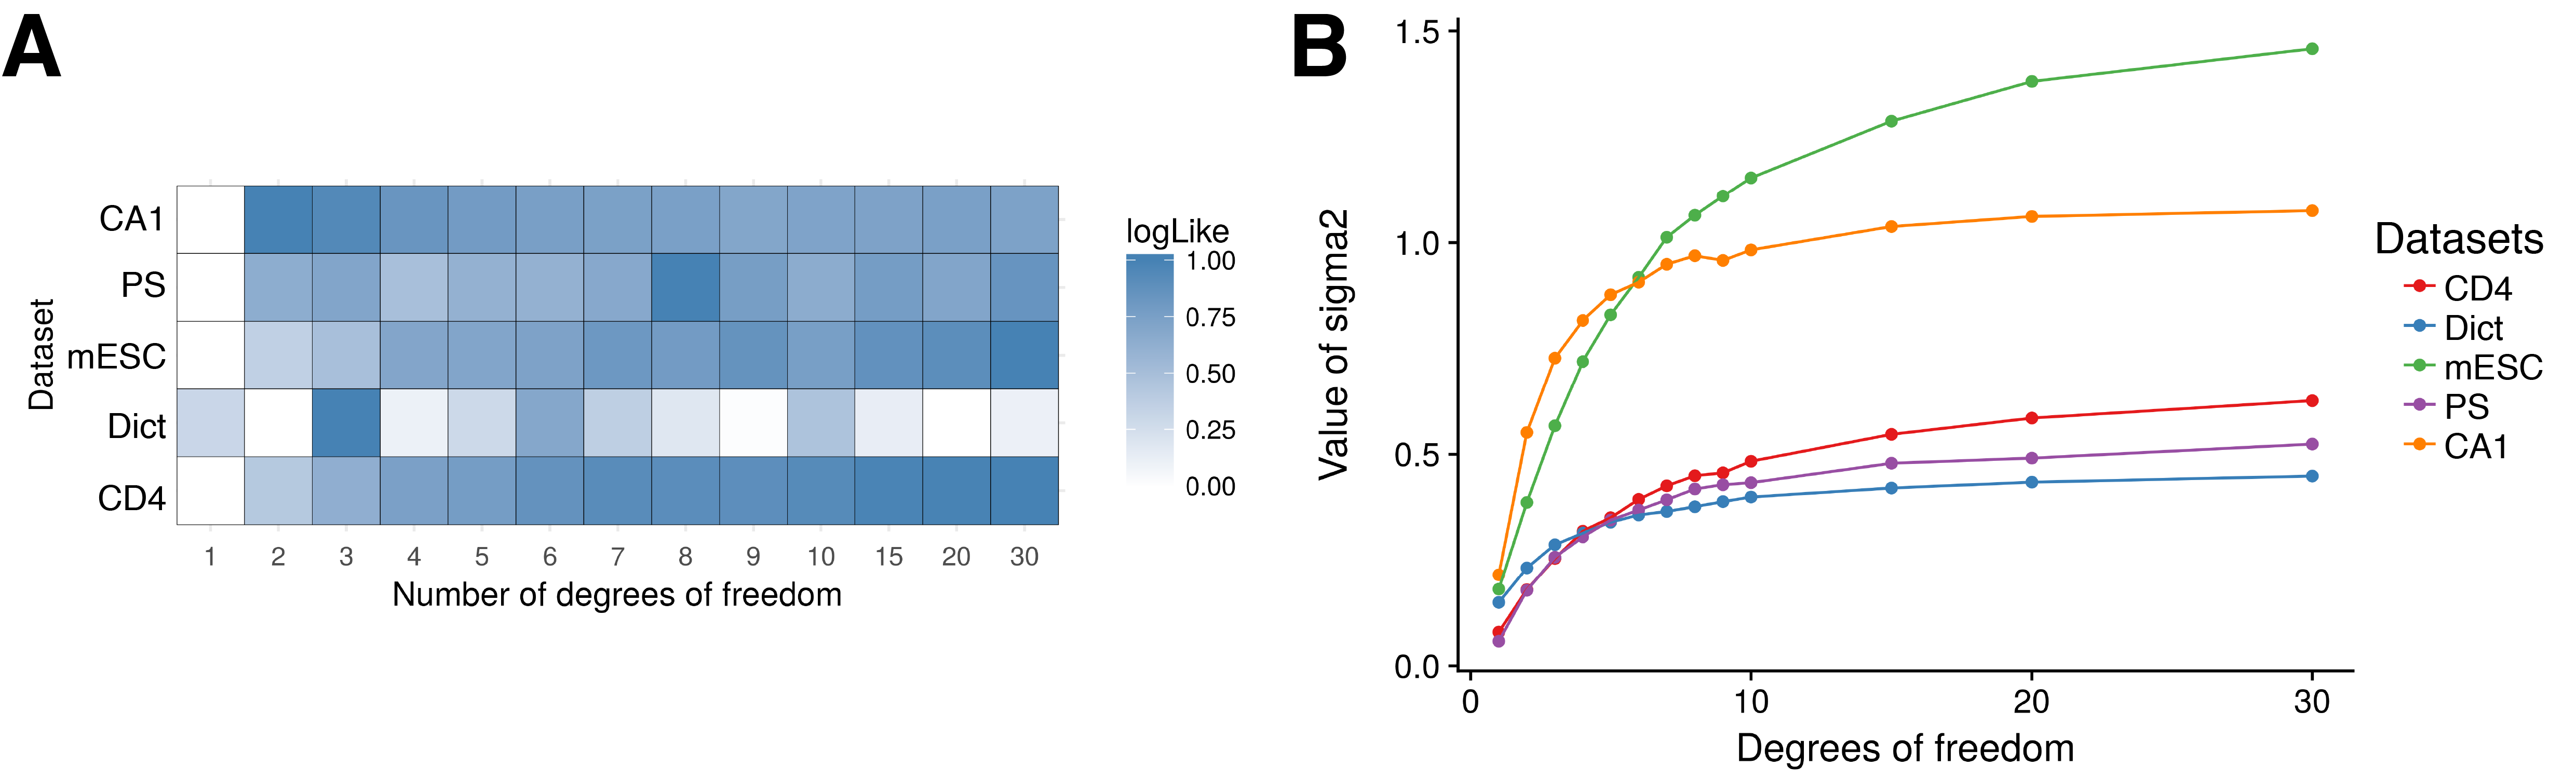
\includegraphics[width=\textwidth]{Fig_5.png}
\caption[Enrichment of under-represented somatic cell types in juvenile samples]{\textbf{Enrichment of under-represented somatic cell types in juvenile samples.} \\
\textbf{(A)} tSNE representation of cells isolated from P10 animals that were mapped to cells from adult mice. Cell types were identified by unbiased, graph-based clustering and annotated after marker gene extraction. SG: Spermatogonia, SC: Spermatocytes, IL: Immature Leydig, PTM: Peritubular Myoid Cells, EC: Endothelial Cells, tMg: testicular Macrophages, \textbf{(B)} Heatmap representation of cell type-specific marker genes. Bolded genes indicate previously described markers for the following cell types: Sertoli cells (\textit{Cst12}), early spermatocytes (\textit{Sycp1}), spermatogonia (\textit{Dmrt1}), immature leydig cells (\textit{Dlk1}), endothelial cells (\textit{Acta2}), peritubular myoid cells (\textit{Tm4sf1}), Leydig cells (Insl3), testicular macrophages (\textit{Cd14}). \textbf{(C)} PCA of spermatogonia (SG) and early spermatocytes (SC 1) from P10 and P15 animals. 
}
\label{fig3:somatic_cells}
\end{figure}

Furthermore, we detect a relative enrichment of spermatogonia compared to other germ cell types at P10 and P15 \textbf{(Fig.~\ref{fig3:somatic_cells}C)}. Using this large amount of stem-cell like cells sampled from different time-points during development allows us to dissect its differentiation programme.

\newpage

\subsection{Spermatogonial differentiation}

In the mouse, spermatogenesis is initiated with the division of a spermatogonial stem cell (SSC or A$_{\text{single}}$) to form first a pair, and then a connected chain of undifferentiated spermatogonia (A$_{\text{paired}}$ and A$_{\text{aligned}}$) \citep{Oakberg1971, DeRooij1973}. These cells have competency to undergo spermatogonial differentiation, which involves six transit-amplifying mitotic divisions generating A$_{1-4}$, Intermediate (In), and B spermatogonia, which then give rise to pre-leptotene spermatocytes (Pl) \citep{DeRooij2000} \textbf{(Fig.~\ref{fig3:cell_staging}C)}. Given this, we expect a high level of heterogeneity within the spermatogonia population but identifying spermatogonial sub-populations in adult testes is greatly complicated by their rarity relative to other germ cell types \citep{Lukassen2018}. However, as shown above, during early juvenile development spermatogonia are relatively enriched, which we exploited to further characterize their heterogeneity \textbf{(Fig. \ref{fig3:1st_wave}A)}. \\

By combining cells from P10 and P15, we obtained 1,186 transcriptional profiles that capture sub-populations during spermatogonial differentiation \textbf{(Fig.~\ref{fig3:spermatogonia}B)}. To jointly analyse transcriptomes of P10 and P15 samples, we performed batch correction between these samples as described above and clustered batch corrected data using a graph-based approach. In order to label the cell types corresponding to the different clusters, we performed marker genes detection using the \emph{findMarker} function in \emph{scran}. By visualizing the individual marker genes, we detect two clusters corresponding to undifferentiated spermatogonia (A$_\textnormal{undiff}$) based on their expression of \textit{Nanos3} and \textit{Zbtb16} \textbf{(Fig. \ref{fig3:spermatogonia}B and C)} \citep{Buaas2004, Lolicato2008}). These cells comprise A$_\textnormal{s}$, A$_\textnormal{paired}$, and A$_\textnormal{aligned}$ spermatogonia that decrease in stemness as they divide and gain competency to differentiate \citep{Suzuki2012}. Additionally, these cells express a number of marker genes also detected in undifferentiated human spermatogonial stem cells, such as \textit{Gfra1}, \textit{Bcl6} and \textit{Id4} \citep{Guo2017}. Based on the expression of \textit{Stra8} (Stimulated by retinoic acid 8), we can map the point at which spermatogonial differentiation is induced (A$_\textnormal{aligned}$-to-A$_\textnormal{1}$ transition), thus marking the beginning of differentiating spermatogonia (A$_\textnormal{diff}$) \citep{Endo2015} \textbf{(Fig. \ref{fig3:spermatogonia}B)}. A$_\textnormal{diff}$ are marked by the expression of \textit{Sohlh1} \citep{Ballow2006} and are highly proliferative, generating A$_\textnormal{1-4}$, Intermediate and B spermatogonia. Late differentiating spermatocytes express \textit{Dmrtb1}, which mediates the mitosis-to-meiosis transition and quickly disappears in pre-leptotene spermatocytes \textbf{(Fig. \ref{fig3:spermatogonia}B)}. This latter population shows a second increase in \textit{Stra8} expression levels, which is necessary for initiation of meiosis \textbf{(Fig.~\ref{fig3:spermatogonia}B and C)} \citep{Anderson2008, Endo2015, Zhang2014}. 

\newpage

\begin{figure}[!h]
\centering
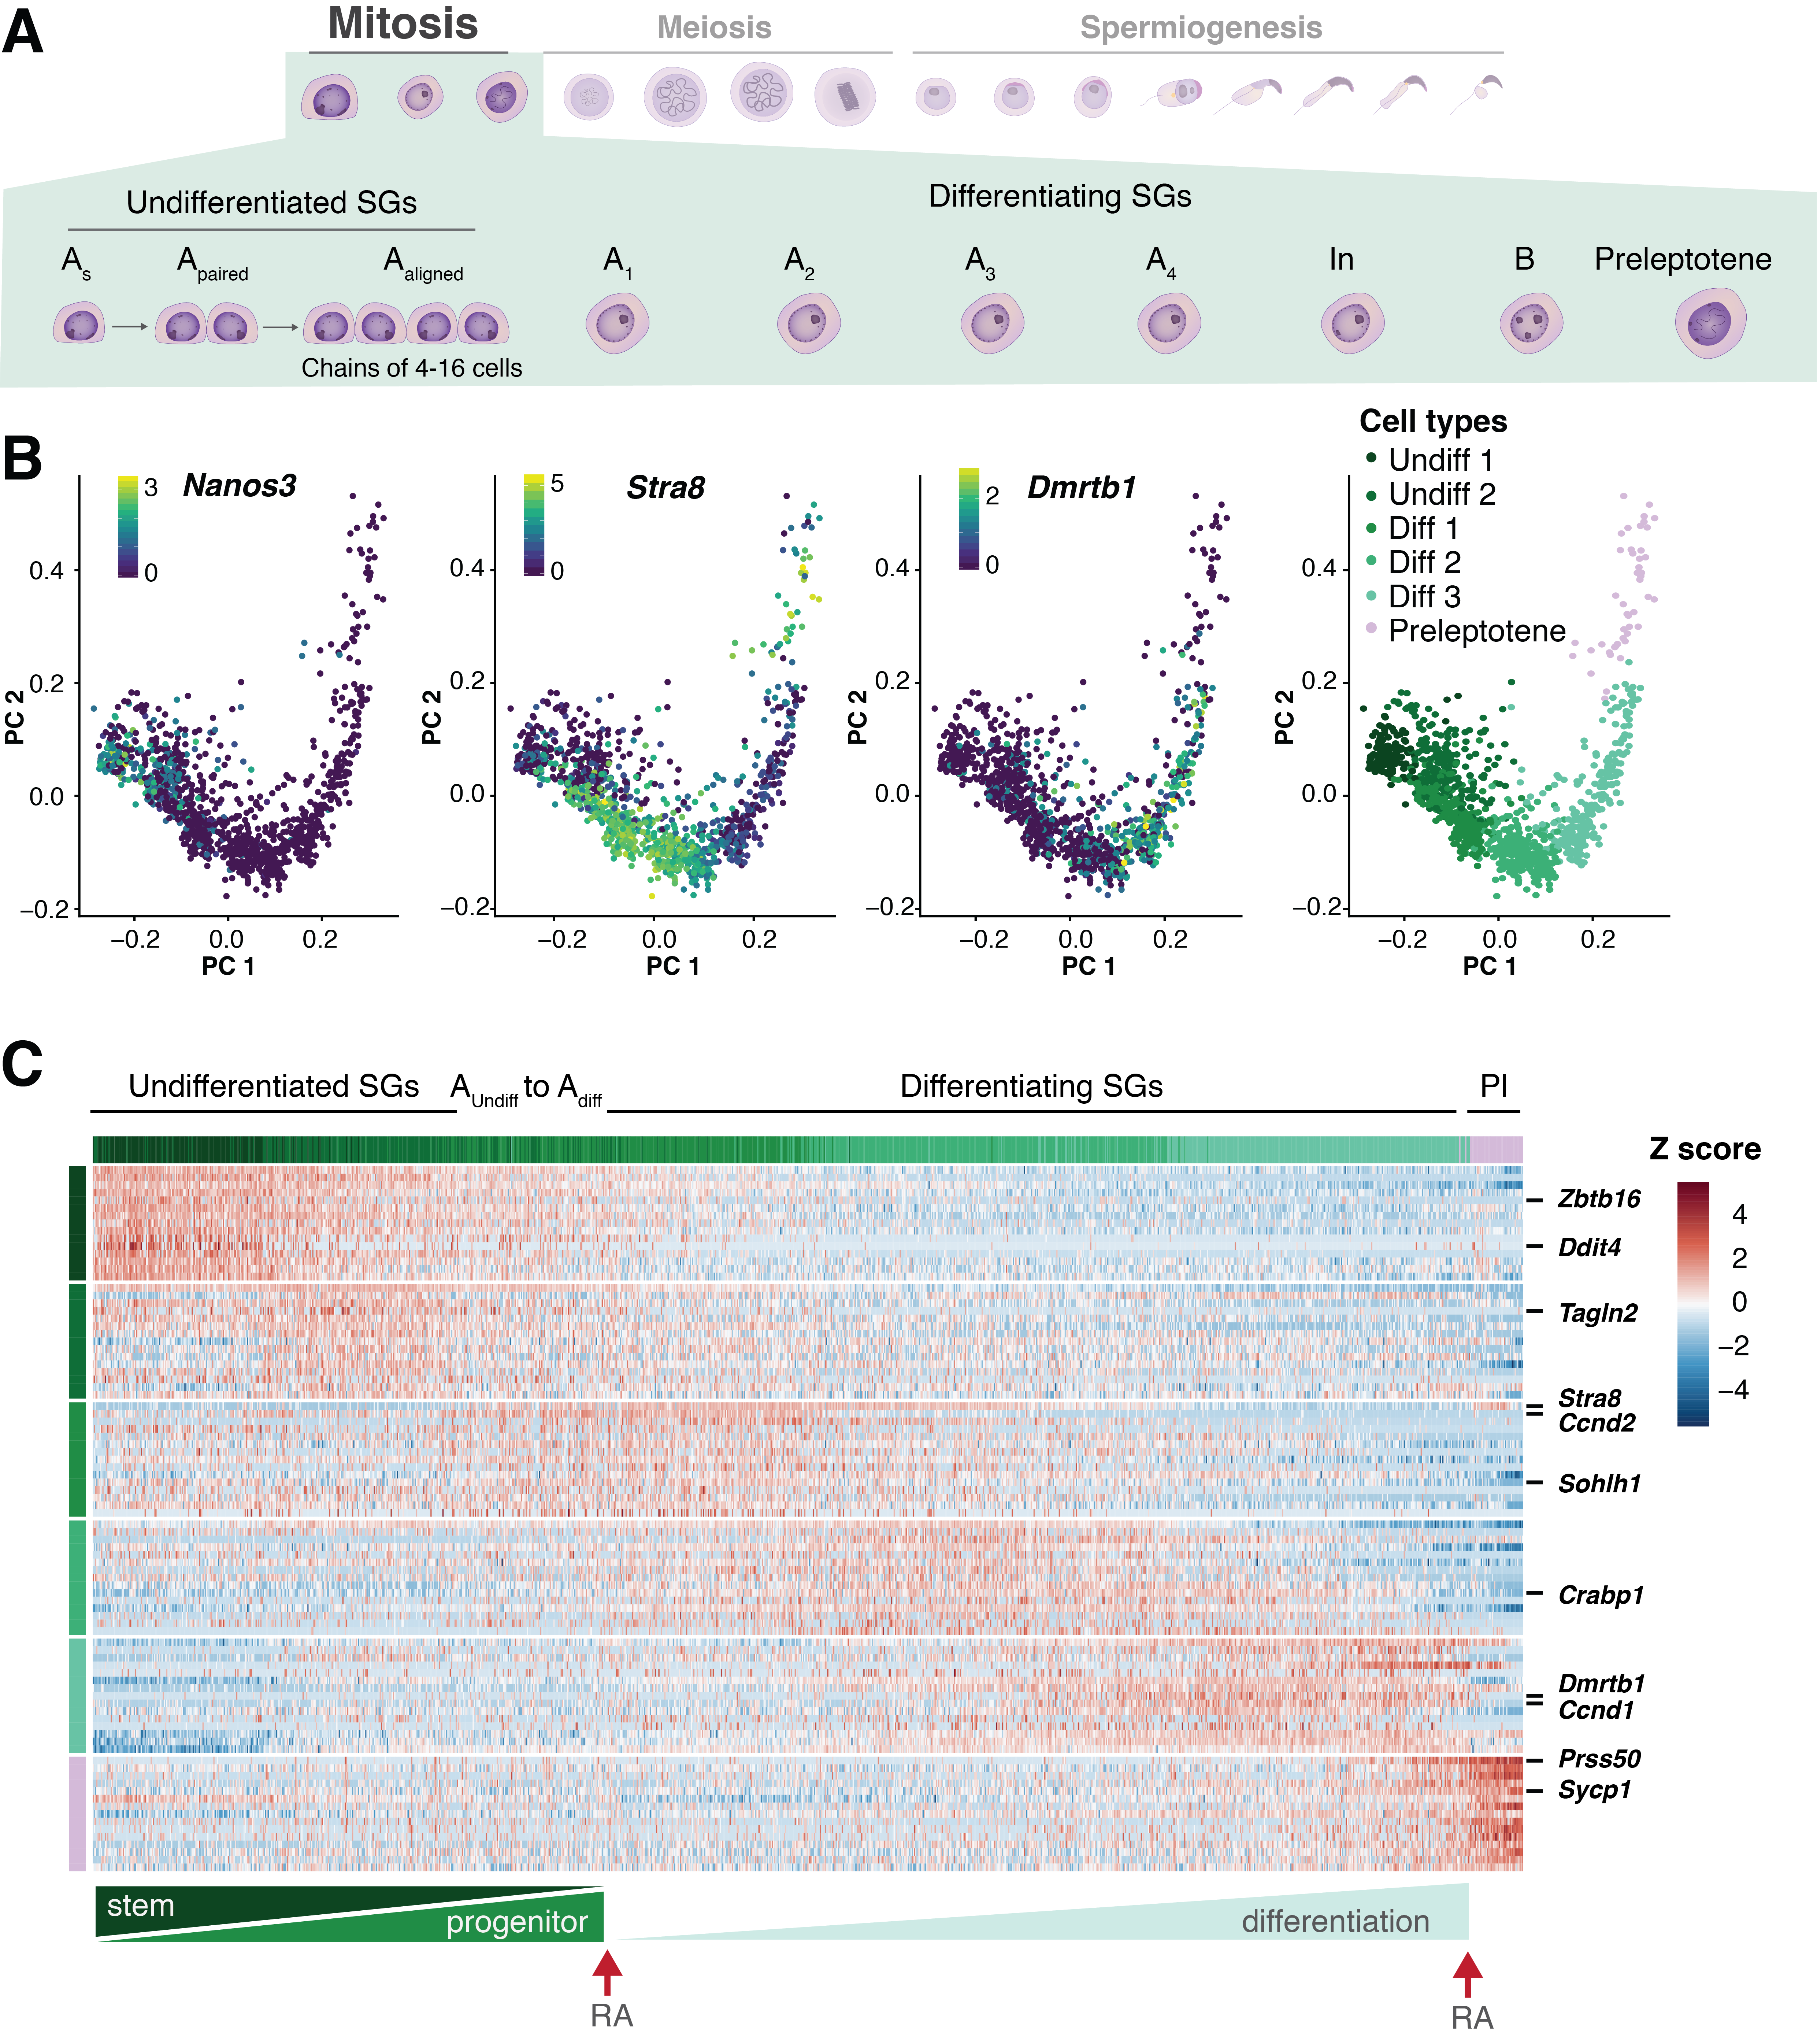
\includegraphics[width=0.9\textwidth]{Fig_6.png}
\caption[Cellular heterogeneity during spermatogonial differentiation]{\textbf{Cellular heterogeneity during spermatogonial differentiation.}\\
\textbf{(A)} Schematic representation of spermatogonial differentiation including sub-stages of undifferentiated (A$_\textnormal{s}$, A$_\textnormal{paired}$, A$_\textnormal{aligned}$) and differentiating (A$_\textnormal{1}$, A$_\textnormal{2}$, A$_\textnormal{3}$, A$_\textnormal{4}$, In, B) spermatogonia (SGs) as well as pre-leptotene spermatocytes (Pl), \textbf{(B)} Sub-structure detection in spermatogonia isolated from P10 and P15 animals. PCA was computed on transcriptomes after batch correction between P10 and P15 samples. The first three panels represent expression of known marker genes for undifferentiated (Undiff, \textit{Nanos3}) and differentiating (Diff, \textit{Stra8} and \textit{Dmrtb1}) spermatogonia. The colour scale shows log$_2$-transformed, normalized counts. The last panel overlays cluster identity by sub-clustering batch-corrected transcriptomes of spermatogonia, \textbf{(C)} Z factor of normalized expression counts of the top 15 marker genes per cell cluster. Column and row labels represent the cell clusters identified in the last panel of (B). The lower bar indicates the gradual differentiation from undifferentiated spermatogonia to pre-leptotene cells driven by two retinoic acid (RA) signals. }
\label{fig3:spermatogonia}
\end{figure}

\newpage

\subsection{Leptotene and zygotene spermatocytes}

The transition between differentiating spermatogonia and spermatocytes is a gradual process that occurs in stage VIII tubules when B spermatogonia divide and form pre-leptotene spermatocytes \citep{Anderson2008, Baltus2006}. When visualizing the first two components of a PCA, we did not observe a continuous differentiation trajectory bridging spermatogonia to spermatocytes \textbf{(Fig.~\ref{fig3:somatic_cells}C)} which indicates a possible loss of cells that characterise the transition between these two cell-types. One possible explanation is that leptotene and zygotene spermatocytes have decreased transcriptional activity \citep{Kierszenbaum1974, Monesi1965}, and are thus likely to be classified as empty droplets by the 10X CellRanger pipeline. \\

To capture these transcriptionally quiescent cells and as explained above, we used the \emph{emptyDrops} function from the \emph{DropletUtils} R package to distinguish between droplets capturing genuine cells with low transcriptional complexity \emph{versus} empty droplets containing only ambient mRNA \citep{Lun2018}. Applying this approach increased the number of early spermatocytes in all samples and, in particular, identified a population of cells connecting spermatogonia and spermatocytes at the predicted position in the cell trajectory \textbf{(Fig.~\ref{fig3:emptyDrops}A-C)}. Especially in the P15 sample, we strongly enrich for leptotene and zygotene spermatocytes when including smaller cells into the analysis. Due to low transcriptional complexity, these two cell-types cluster together which makes it hard to detect a clear mitosis-to-meiosis transition \textbf{(Fig.~\ref{fig3:emptyDrops}B and C)}. As expected for leptotene and zygotene spermatocytes, these cells show high mRNA levels for genes involved in synaptonemal complex formation, chromosome synapsis and DNA double-strand break (DSB) formation such as \textit{Sycp1}, \textit{H2afx} and \textit{Hormad1} \citep{Daniel2011, Mahadevaiah2001, Vries2005} \textbf{(Fig.~\ref{fig3:emptyDrops}D)}.\\

In addition to early spermatocytes, droplets with lower transcriptional complexity also captured late condensing spermatids. As mentioned above, these late stages of spermiogenesis are characterized by continuous degradation of RNA after transcriptional shut-down at the round-to-elongating transition \citep{Steger1999} \textbf{(Fig.~\ref{fig3:emptyDrops}E)}. Nevertheless, including droplets with low transcriptional complexity increases the risk of including low-quality cells and debris. In our case, the large cluster of unidentified cells in \textbf{Fig.~\ref{fig3:emptyDrops}A} could represent membrane vesicles containing RNA at the end of spermiogenesis that form during a process termed "cytoplasmic extrusion" \citep{Rengan2012}.\\

\newpage

\begin{figure}[!h]
\centering
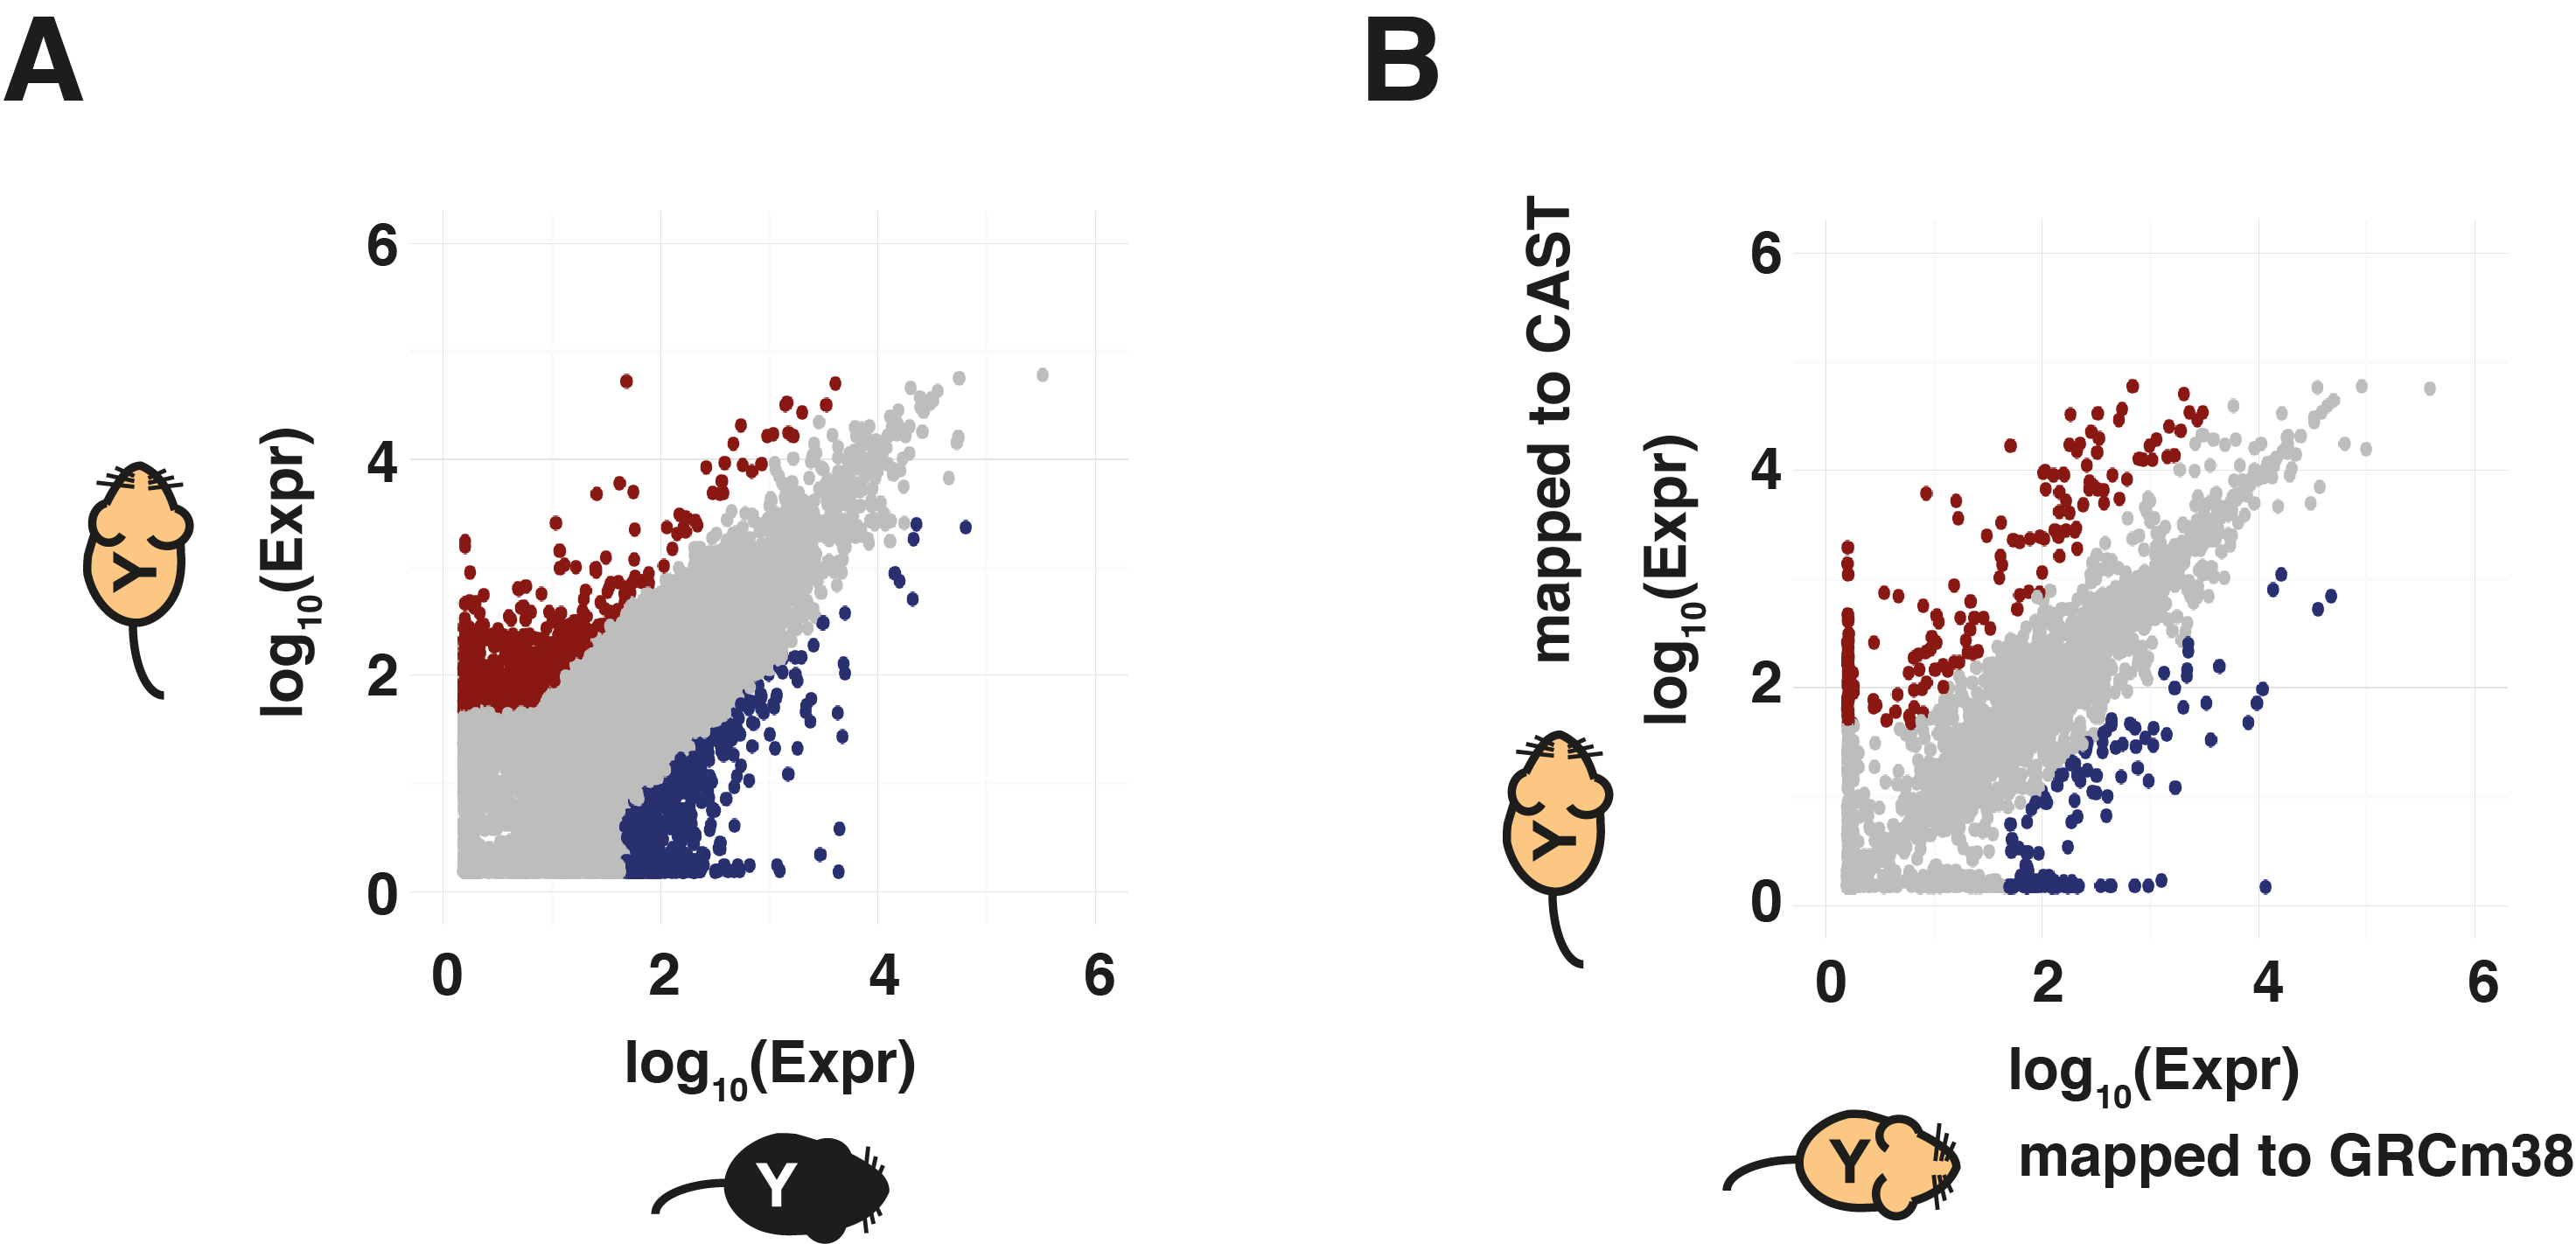
\includegraphics[width=0.8\textwidth]{Fig_7.png}
\caption[Transcriptionally silent cell types in spermatogenesis.]{\textbf{Detection of transcriptionally silent cell types in scRNA-Seq data.} \\
\textbf{(A)} tSNE representation of cells selected by the \emph{emptyDrops} filtering strategy. Coloured dots represent annotated cell types detected using the default \emph{CellRanger} filtering pipeline while black dots represent cells detected by the \emph{emptyDrops} filtering. SG: Spermatogonia, SC: Spermatocytes, IL: Immature Leydig, PTM: Peritubular Myoid Cells, EC: Endothelial Cells, tMg: testicular Macrophages, \textbf{(B)} tSNE representation of emptyDrops filtered cells from the P15 sample. Cell colouring corresponds to clustering performed on this sample. Undiff SG: undifferentiated spermatogonia, Diff SG: differentiating spermatogonia, \textbf{(C)} PCA representation of spermatogonia and spermatocytes detected in the P15 sample after \emph{emptyDrops} filtering. Labelling corresponds to the clusters shown in (B), \textbf{(D)} Leptotene and zygotene spermatocyte marker gene expression. The colour scale represents log$_2$-transformed, normalized counts, \textbf{(E)} Visualization of the number of genes expressed (> 0 counts) per cell.}
\label{fig3:emptyDrops}
\end{figure}

\newpage

\section{Characterization of male meiosis}

After characterising the major germ and somatic cell types, we next profiled the transcriptional programmes of known developmental processes during spermatogenesis. These include firstly meiosis and later on spermiogenesis which will be analysed and discussed in the next section.\\

The mitotic expansion of spermatogonia produces large numbers of spermatocytes, which then undergo male meiosis where two consecutive cell divisions give rise to four haploid spermatids. In contrast to mitotic cell divisions, prophase of meiosis I is extremely prolonged, lasting up to 10 days in male mice \citep{Soh2017}. Furthermore, meiosis includes programmed DNA double strand break (DSB) formation, homologous recombination, and chromosome synapsis \citep{Marston2004}, which represent molecular processes to induce genetic variation between offsprings. Most meiotic processes have been histologically described, but a full transcriptional characterization of spermatocytes undergoing meiosis is lacking. \\

The continuum of sampled cell types allows us to perform in-depth characterisation of transcriptional changes that occur during meiosis. For this, we ordered spermatocytes along their differentiation trajectory by fitting a principal curve \citep{Hastie1989} to the first 3 principal components using the \emph{principal.curve} function implemented in the \emph{princurve} R package. This approach allows us to order cells along the developmental trajectory. The directionality of the trajectory was inferred using prior information based on the cluster annotation. Here, the ordering of cell types is as follows: leptotene spermatocytes (SCs, not present in CellRanger filtered data), zygotene SCs, pachytene SCs, diplotene SCs and finally cells in metaphase \textbf{(Fig.~\ref{fig3:meiosis}A)}. \\

To detect molecular processes that occur during meiosis, we first profiled the overall transcriptional rate before dissecting changes in expression on a gene-specific level. As shown before \citep{Xia2018}, we identified a strong increase in the number of genes expressed as spermatocytes progress through prophase, with the highest number being expressed immediately before the cells divide \textbf{(Fig.~\ref{fig3:meiosis}A)}. Using this as a proxy for active transcription, we identified diplotene spermatocytes, which are the latest cell type in prophase I in which RNA synthesis is occurring \citep{Monesi1965}. 

\newpage

We used the increase and later decrease in transcription as a guide for the progressive changes in transcription throughout meiosis. Therefore, to detect functional genes that influence this process, we correlated each gene’s normalised expression level to the number of genes expressed. For this, we used the \emph{correlatedPairs} function implemented in \emph{scran} \citep{Lun2016}. First, we constructed an empirical null distribution using the \emph{correlateNull} function implemented in \emph{scran}. Next, we tested the observed Spearman’s $\rho$ for each gene against this null distribution. Genes with $\rho$ < -0.3 and a Benjamini-Hochberg corrected empirical p-value < 0.1 were considered as negatively correlated and genes with $\rho$ > 0.3 and a Benjamini-Hochberg corrected empirical p-value < 0.1 were considered as positively correlated.\\

As expected, previously known marker genes for early meiotic processes such as \textit{Hormad1} and \textit{Sycp3} decreased in expression during Prophase I, whereas \textit{Pou5f2} and \textit{Tcte2}, a male-meiosis specific gene \citep{Braidotti1997} increased in expression \textbf{(Fig.~\ref{fig3:meiosis}B)}. Supporting our identification of diplotene spermatocytes, \textit{Pou5f2} has previously been shown to be specifically expressed during a 36- to 48-hour period preceding the meiotic cell division \citep{Andersen1993}. \\

In the next step, we performed less biased analysis and detected marker genes for each of the spermatocyte sub-cell-types. Despite the overall increase in transcription, we observed distinct temporal expression patterns when visualizing these specific marker genes for individual spermatocyte populations. Even within pachytene spermatocytes at different stages in their developmental progression, there exists substantial heterogeneity \textbf{(Fig.~\ref{fig3:meiosis}C)}. As expected, early spermatocyte markers (SC 1 and SC 2) were enriched for genes with known functions in male or female fertility such as \textit{Piwil1} (\textit{Miwi}), \textit{Cks2}, \textit{Sycp1}, reflecting a history of intensive investigation \citep{Deng2002, Spruck2003, Vries2005}. We performed literature search and used the database \url{www.mousephenotype.org} to annotated genes regarding their sterility phenotype. \\

In sum, we dissected the transcriptional heterogeneity within spermatocytes undergoing meiosis and found numerous genes to be associated with this developmental process.

\newpage

\begin{figure}[!h]
\centering
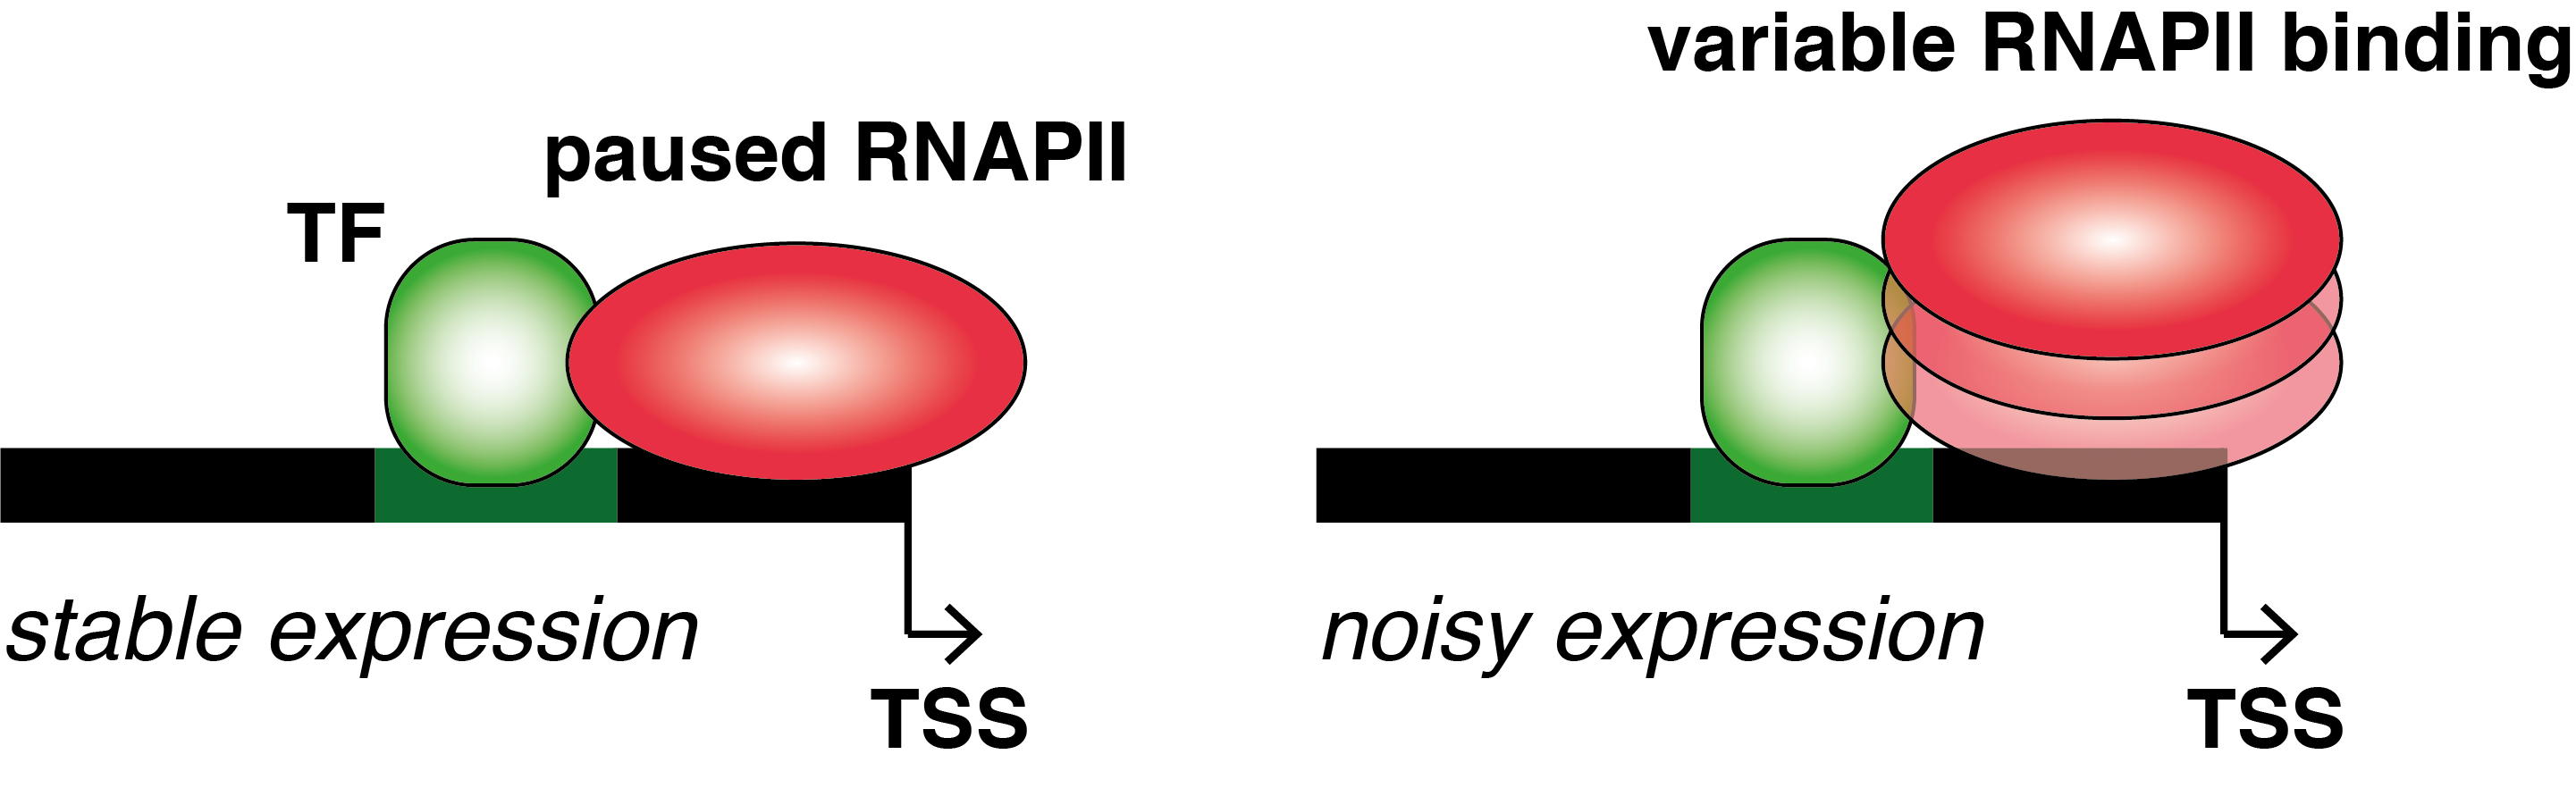
\includegraphics[width=0.9\textwidth]{Fig_8.png}
\caption[Gene expression dynamics during male meiosis]{\textbf{Gene expression dynamics during male meiosis.} \\
\textbf{(A)} Number of genes expressed per spermatocyte. Cells are ordered by their developmental progression during meiotic prophase until metaphase, \textbf{(B)} Expression of genes that are negatively or positively correlated with the number of genes expressed during meiotic prophase (negatively correlated: $\rho$ < -0.3, Benjamini-Hochberg corrected empirical p-value < 0.1; positively correlated: $\rho$ > 0.3, Benjamini-Hochberg corrected empirical p-value < 0.1). Per category, two genes are visualized. The colour gradient represents log$_2$-transformed, normalized counts, \textbf{(C)} Heatmap visualizing the Z factor scaled expression of the top 15 marker genes per cell type. Row and column labels correspond to the different populations of spermatocytes (SC). M: Metaphase. Genes are labelled based on their fertility phenotype: pink – infertile or sub-fertile in females, light blue - infertile or sub-fertile in males, dark green - infertile or sub-fertile in both males and females. The sterility phenotype was annotated using \url{www.mousephenotype.org.}}
\label{fig3:meiosis}
\end{figure}

\section{Transcriptional dynamics during spermiogenesis}
\label{sec3:spermiogenesis}

Once the meiotic divisions resulted in the production of four haploid cells, round spermatids progress to form first elongating and finally mature sperm during a process termed "spermiogenesis" \textbf{(Fig.~\ref{fig3:spermiogenesis}A)}. A key event during spermiogenesis is chromatin condensation, which is required to package the haploid genome into the confined space of the sperm nucleus. Our data allowed us to dissect at high-resolution the transcriptional regulation needed for gradual chromatin remodelling during spermatid differentiation, involving the replacement of canonical histones by histone variants followed by transition proteins and eventually protamines \citep{Balhorn2007, Kennani2017}. This chromatin remodelling later on induces a transcriptional shut-down where changes in RNA content are purely driven by degradation \citep{Steger1999}.

\subsection{Expression of chromatin components during spermiogenesis}

For this, we first explored how expression of histone variants changed throughout early spermatid maturation \textbf{(Fig.~\ref{fig3:spermiogenesis}A)}. Similar to the developmental ordering presented in the previous section, we ordered cells by fitting a principle curve to the first three principal components calculated on S1-S14 spermatids. Annotations for histone variants and canonical histones were taken from El Kennani \emph{et al.}, 2017 \citep{Kennani2017}. Multiple variants of H3 and H2A are expressed in spermatocytes \citep{Greaves2006, Mahadevaiah2001, Tang2015}, and our data showed that many of these histones are highly expressed in early round spermatids. For instance, Histone H3.3 is a histone variant consisting of two genomic copies (\textit{H3f3a} and \textit{H3f3b}). Across spermatogenesis, we observed distinct expression patterns for the two genes, with \textit{H3f3a} being consistently high until the transcriptional shut-down at spermatid stage S10. In contrast, \textit{H3f3b} showed a much more dynamic expression profile, starting high in spermatocytes, dropping throughout meiotic prophase, followed by up-regulation in round spermatids \textbf{(Fig.~\ref{fig3:spermiogenesis}B)}. Although both genes have been implicated in male fertility, the phenotypes associated with perturbations of the more dynamically regulated paralog \textit{H3f3b} are much more severe \citep{Tang2015, Yuen2014}.\\

When profiling the expression of canonical histones, we detected increased expression for \textit{Hist1h2bp} and \textit{Hist1h4a} that showed a distinct up-regulation during early and mid-spermiogenesis \textbf{(Fig.~\ref{fig3:spermiogenesis}C)}. Canonical histones are typically transcribed in a replication-dependent manner during S phase \citep{Marzluff2002}, thus the atypical expression during spermiogenesis could suggest important roles as replacement histones during chromatin remodelling. Nevertheless, canonical histones appeared to be the set of annotated histones that is least correlated to the developmental trajectory \textbf{(Fig.~\ref{fig3:spermiogenesis}A)}.

\newpage

\begin{figure}[!h]
\centering
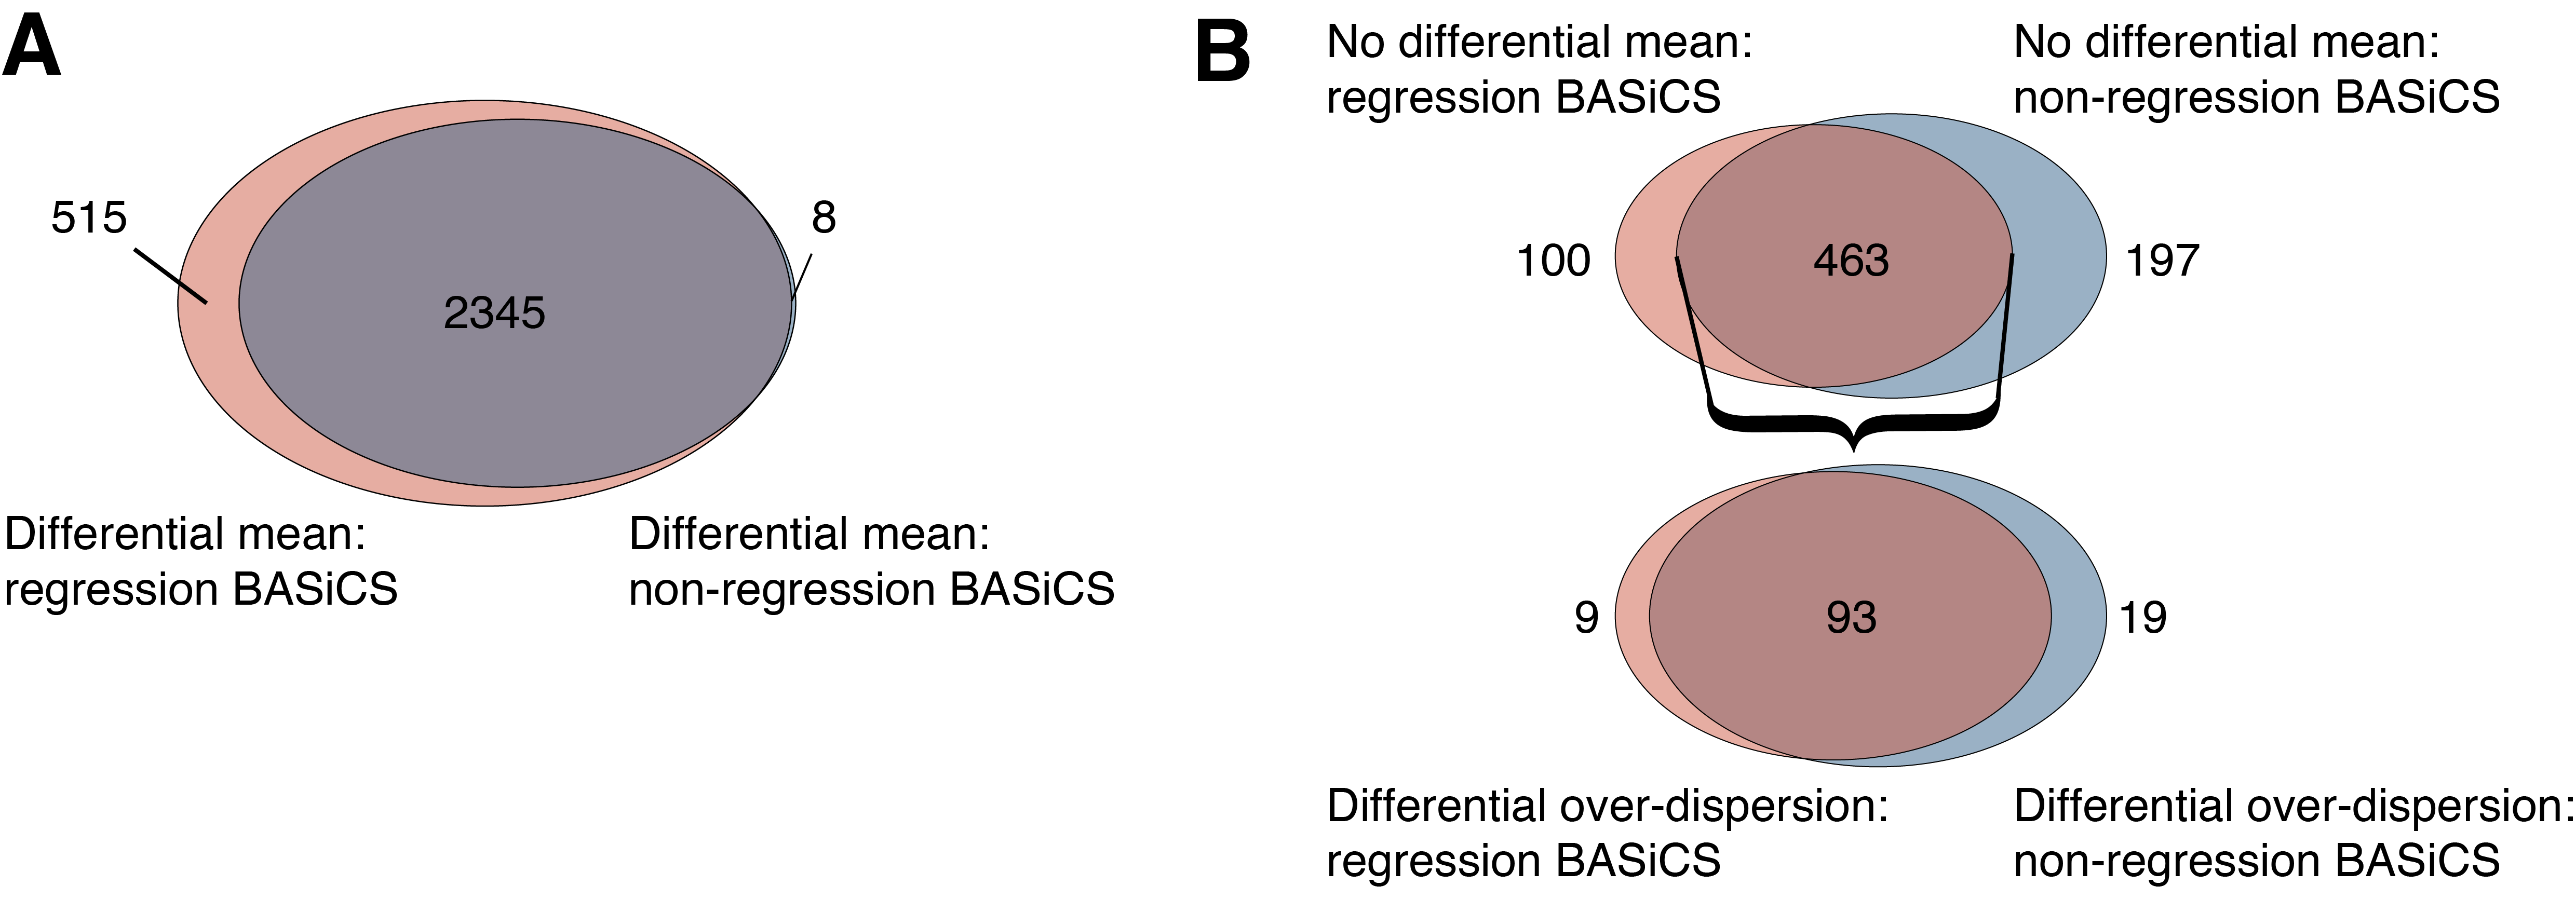
\includegraphics[width=0.85\textwidth]{Fig_9.png}
\caption[Transcriptional dynamics and chromatin remodelling during spermiogenesis]{\textbf{Transcriptional dynamics coupled to chromatin remodelling during spermiogenesis.} \\
\textbf{(A)} Z factor scaled, normalized expression of histone variants (H1, H2A, H2B, H3), canonical histones, transition proteins (Tnp) and protamines (Prm) during spermiogenesis. Cells were ordered based on their developmental trajectory ranging from round spermatids (S1-S8) to elongating spermatids (S9-S14), \textbf{(B)} Expression of \textit{H3f3a} (middle panel) and \textit{H3f3b} (right panel) across the different germ cell populations, \textbf{(C)} Similar visualization as in (B) for \textit{Hist1h4a} expression across germ cells. }
\label{fig3:spermiogenesis}
\end{figure}

\newpage

We next profiled the transcriptional dynamics of testis-specific histone variants. They showed highest expression in elongating spermatids, with most variants increasing strongly in expression from S5 onwards. While some variants had a consistently high expression level, \textit{Hils1} and \textit{H1fnt} decreased in expression towards the late stages, similarly to \textit{Tnp1} and \textit{Tnp2} \citep{Zhao2004}. Both histone variants are important for male fertility, and \textit{Hils1} has previously been shown to interact with \textit{Tnp1} \citep{Tanaka2005}. In contrast, three testis-specific histone variants \textit{Hypm}, \textit{H2afb1} and \textit{H2bl1} (\textit{1700024p04rik}) showed consistently high expression until the end of differentiation similar to protamines, suggesting these variants contribute to the final genome condensation.

\subsection{Identifying the point of transcriptional shut-down}

As a consequence of chromatin condensation, transcription ceases in spermatids at the round to elongating switch, consistent with the lack of active RNA Pol II at S10 and later stages \citep{DottermuschHeidel2014}.
By fitting a smooth regression (loess) to the number of genes expressed per cells along the differentiation trajectory, we easily identified the point of transcriptional shut-down. The number of expressed genes is stable until approximately S9 before gradually declining by roughly 50\% \textbf{(Fig.~\ref{fig3:transcriptional_shutdown}A)}. In the 8 days following transcriptional shut-down, spermatids still need to undergo drastic morphological changes, including the assembly of sperm-specific structures such as the flagellum, before mature testicular sperm can be released into the lumen \citep{ODonnell2014}. To achieve this in the absence of active transcription, spermatids store large amounts of mRNAs in a perinuclear RNA granule termed the chromatoid body or \emph{nuage} \citep{Kotaja2007}. RNA stored in the chromatoid body is then released for translation, suggesting that these molecules may play vital roles during late stages of spermiogenesis. However, identifying the RNAs that are stored has been hindered by difficulties in purifying late spermatids. \\

By correlating normalized gene expression against the number of genes expressed, we identified a large number of genes that gradually decrease in relative expression after transcriptional shut-down. We reasoned that transcripts where the relative expression after transcriptional shut-down appeared to increase are likely protected from degradation \textbf{(Fig. \ref{fig3:transcriptional_shutdown}B)}. This included genes with well-known spermiogenesis-specific functions. Among those that relatively increase in expression, we find transition proteins and protamines that are involved in chromatin condensation. Furthermore, we detect genes that are involved in the development of sperm motility such as \textit{Akap4} and \textit{Cabs1} \citep{Kawashima2009, Miki2002}. 

\newpage

\begin{figure}[!h]
\centering
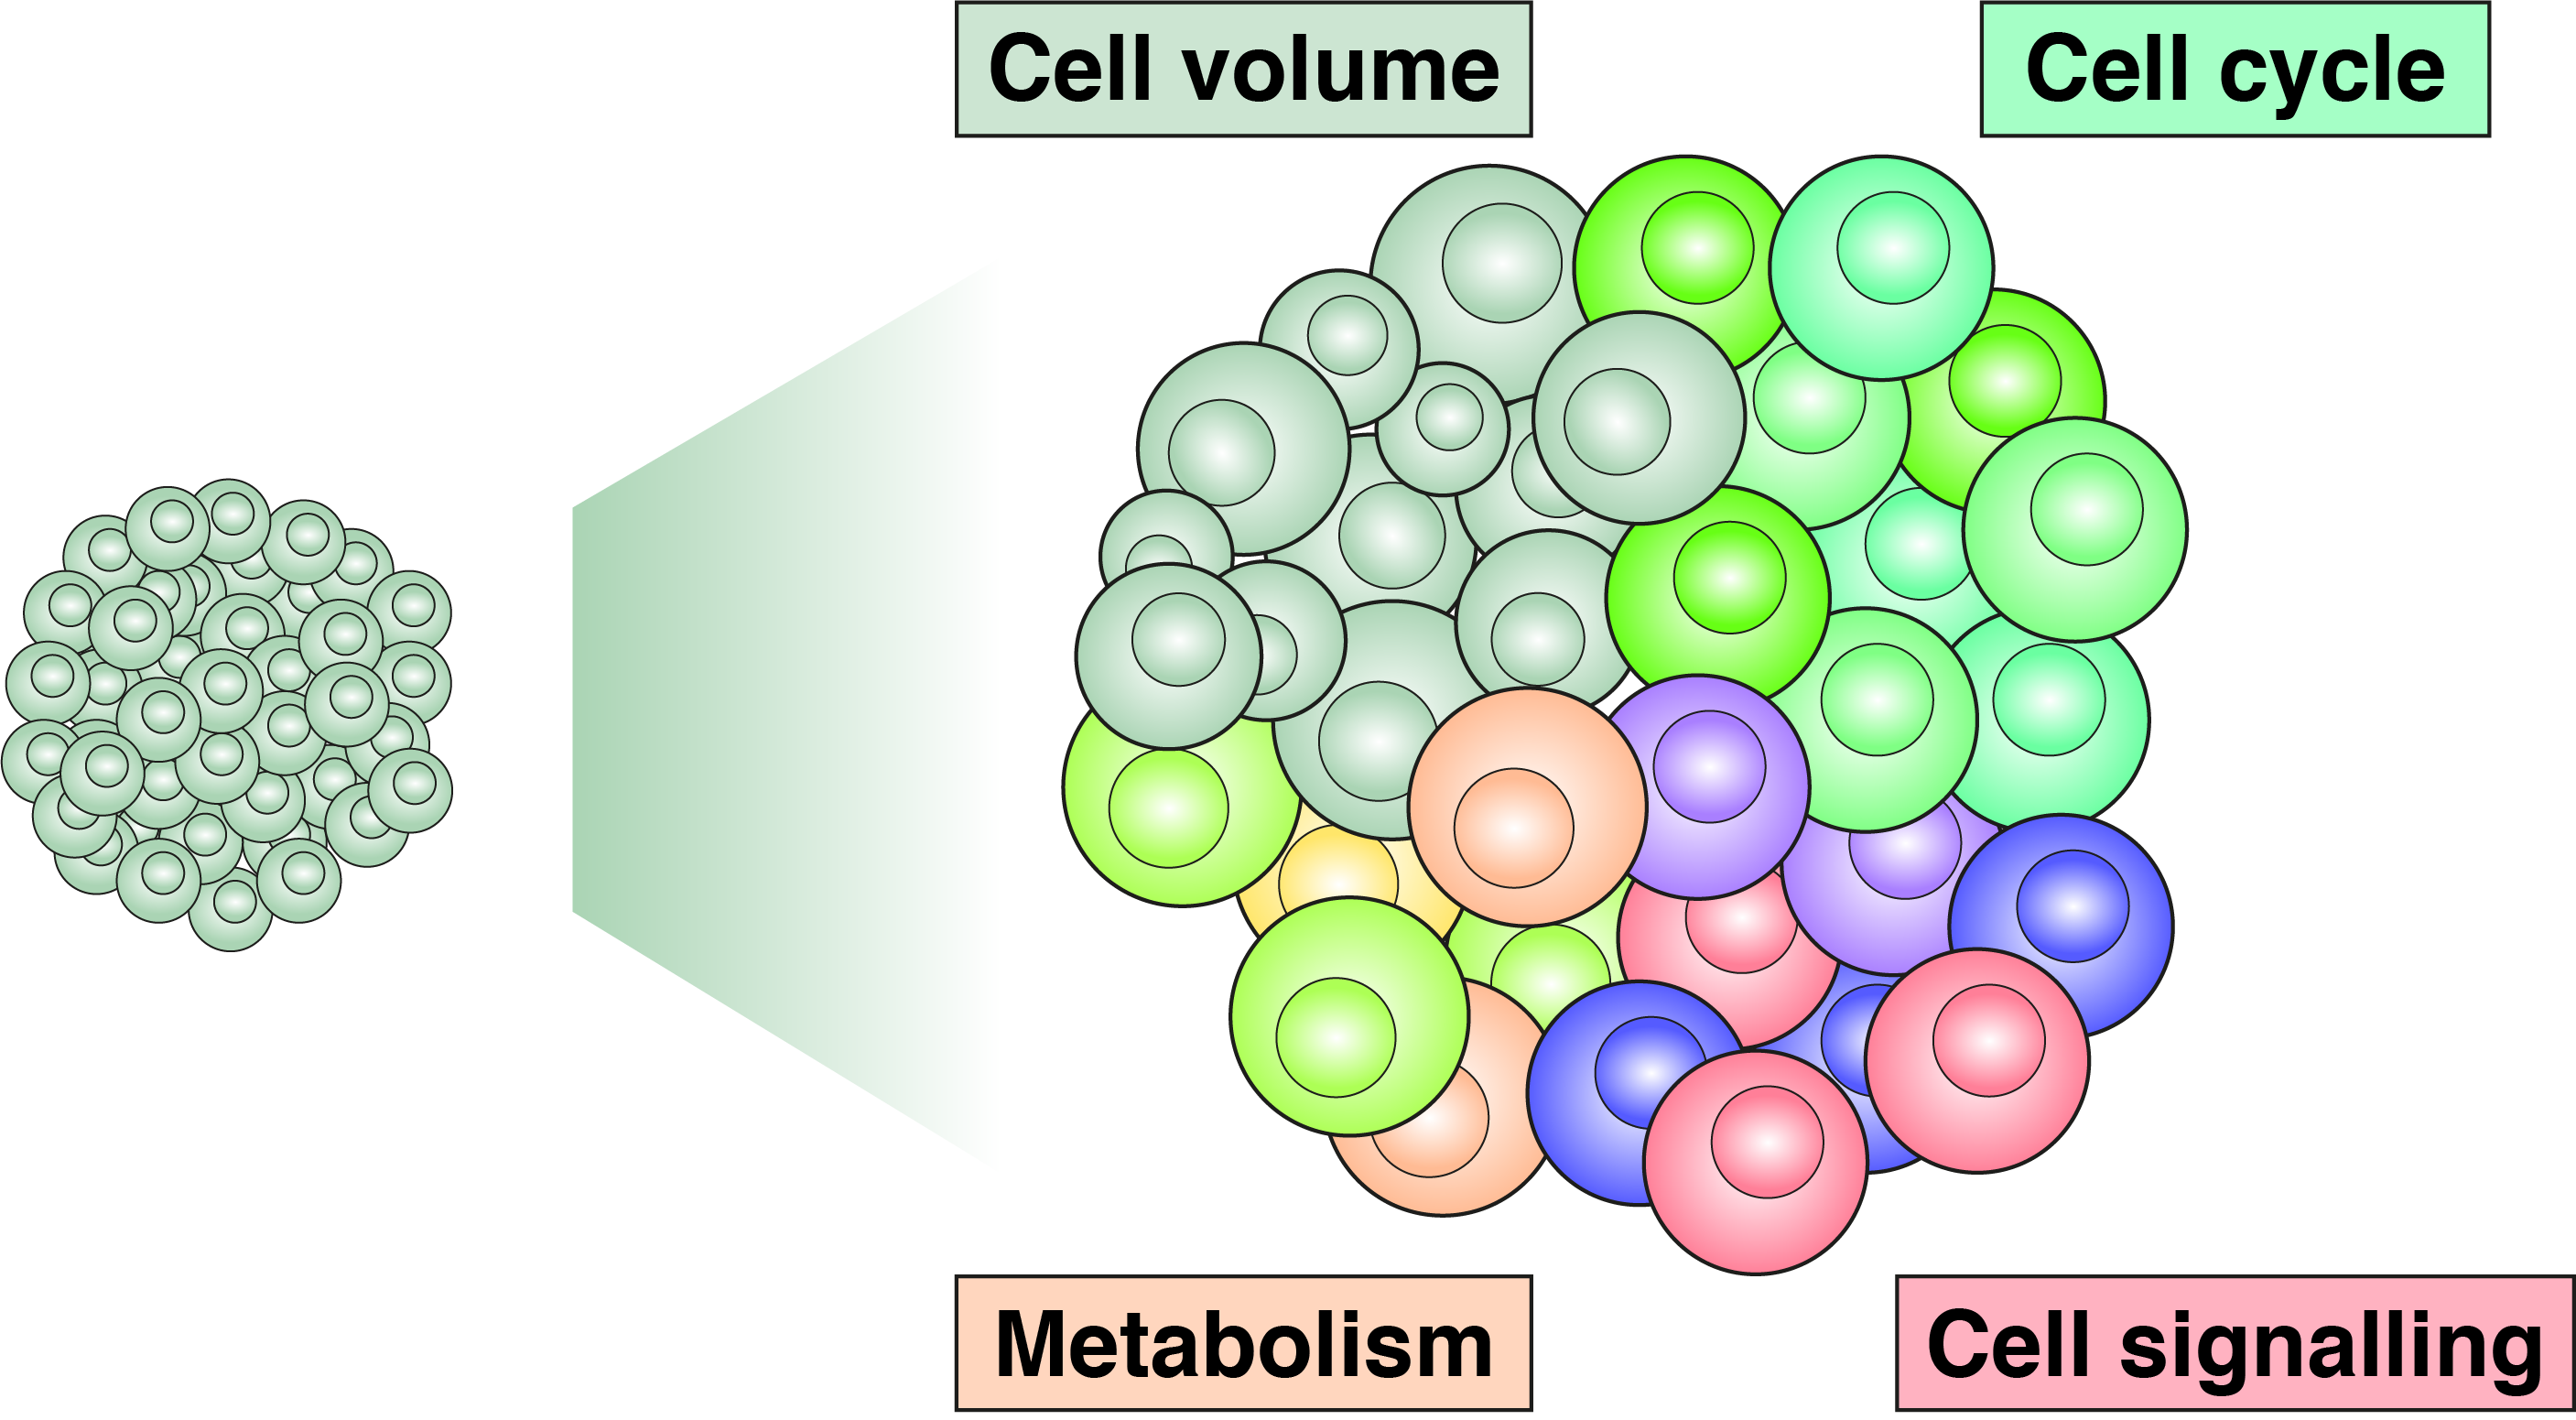
\includegraphics[width=\textwidth]{Fig_10.png}
\caption[Transcriptional shut-down during spermiogenesis]{\textbf{Transcriptional shut-down during spermiogenesis.} \\
\textbf{(A)} Number of genes expressed per spermatid. Cells were ordered based on their developmental trajectory. Red line indicates a smooth regression (loess) fit, \textbf{(B)} For each gene, its normalised expression per cell was correlated with the number of genes expressed per cell. Genes were ordered based on the correlation coefficient and grouped into 9 sets. Z factor scaled expression was averaged across genes within each gene set. Vertical dashed line indicates transcriptional shut-down between S9 and S10.}
\label{fig3:transcriptional_shutdown}
\end{figure}

With this analysis, we explored transcriptional processes occurring throughout the process of spermiogenesis that (i) regulate the expression of chromatin components and (ii) lead to the degradation of unneeded transcripts.

\newpage

\section{Meiotic silencing dynamics of sex chromosomes}

A male-specific feature of meiosis is the transcriptional silencing of sex chromosomes, followed by partial reactivation in post-meiotic spermatids. This process is termed meiotic sex chromosome inactivation (MSCI), and is caused by asynapsis of the sex chromosomes, leading to accumulation of phosphorylated H2AFX and the formation of the sex body \citep{Hamer2003} \textbf{(Fig.~\ref{fig3:X_reactivation}A)}. We next profiled transcriptional changes mediated by the inactivation and reactivation of the sex chromosomes in single-cell and bulk RNA-Seq data. \\

To assess overall transcriptional dynamics of the sex chromosomes, we computed the ratio of expression from the X, Y chromosome and chromosome 9 to all autosomes. For this, we selected genes that were expressed in more than 30\% of spermatogonia or 30\% of spermatids, the cell types with detectable sex chromosome expression. For each cell, the mean expression across these genes per chromosome was calculated. Mean expression of the sex chromosomes and chromosome 9 was divided by mean expression across all autosomes. By plotting the ratio of gene expression from the X or Y chromosomes compared to all autosomes, the inactivation and re-activation status of the sex chromosomes can be inferred \textbf{(Fig.~\ref{fig3:X_reactivation}B)}. \\

The X chromosome is partially up-regulated in spermatogonia as described by Sangrithi \emph{et al.}, 2017 (X:A ratio < 1) \citep{Sangrithi2017}, followed by transcriptional silencing in spermatocytes. Throughout spermiogenesis, expression from the X gradually increases, reaching X:A ratios comparable to spermatogonia, therefore suggesting a substantial reactivation of the X chromosome in post-meiotic spermatids. We detect similar behaviour for the Y chromosome but due to the small number of expressed genes, the signal is noisier \textbf{(Fig.~\ref{fig3:X_reactivation}B)}. In comparison, chromosome 9 shows consistent expression across all cell types throughout spermatogenesis (9:A $\approx$ 1).\\

Transcriptional silencing was originally thought to persist throughout post-meiotic development \citep{Greaves2006, Turner2006}. However, several genes have been shown to be re- or \emph{de novo} activated in spermatids, some of which are dependent on \textit{Rnf8} (Ring finger protein 8) and/or \textit{Scml2} (Sex comb on midleg-like 2) \citep{Hasegawa2015, Sin2012, Sin2015}. The precise timing and order of the transcriptional reactivation of \emph{de novo} escape genes during spermiogenesis has not been explored. We therefore first classified \emph{de novo} activated escape genes using bulk RNA-Seq data and profiled their temporal expression directly following meiosis.\\

Profiling whole-testis transcriptomes of juvenile mice sampled every two days during the first wave of spermatogenesis allowed the sensitive detection of spermatid-specific escape genes \textbf{(Fig.~\ref{fig3:cell_staging}A)}. Due to the gradual emergence of germ cell types during the first spermatogenic wave, differential expression analysis between early ($\leq$ P20) and late (> P20) time points revealed genes exclusively expressed in spermatids and which are thus \emph{de novo} activated escape genes (n = 128) \textbf{(Fig.~\ref{fig3:X_reactivation}C)}. We used \emph{edgeR} to identify differentially expressed genes between these conditions \citep{Robinson2009}. Spermatid-specific genes are identified with a log$_2$-fold change > 5 in samples after day 20 compared to samples before day 20 (controlling the FDR to 10\%). \\

Within the set of \emph{de novo} activated escape genes we find many of the previously annotated escape genes such as \textit{Cypt1}, \textit{Cycl1}, and \textit{Akap4}. Interestingly, this set of genes show an enrichment for targets of H3K27 acetylation which is mediated by \textit{Rnf8} or \textit{Scml2} (Fisher's Exact Test: \textit{Rnf8}-targets, p-value < 5x10$^{-12}$; \textit{Scml2}-targets, p-value < 2x10$^{-9}$) \textbf{(Fig. \ref{fig3:X_reactivation}C)}. This chromatin mark represents active enhances necessary for the reactivation of gene expression in spermatids \citep{Adams2018}. \\

While the bulk RNA-Seq data is ideal to identify spermatid-specific, \emph{de novo} activated genes, it lacks the temporal resolution to differentiate between early and late reactivated genes. We therefore ordered the 128 emph{de novo} activated genes based on their peak in expression using the scRNA-Seq data \textbf{(Fig. \ref{fig3:X_reactivation}D)}. The \emph{de novo} activated genes across our single cell RNA-Seq dataset showed a broad range of temporal expression patterns. The earliest expression, directly following meiosis and lasting until stages S4-S5 was observed for three members of the \textit{Ssxb} multi-copy gene family (\textit{Ssxb1}, \textit{Ssxb2}, \textit{Ssxb3}). Multi-copy genes have previously been described to have spermatid-specific expression \citep{Mueller2008}, and their ampliconic structure has been speculated to play a role in escaping meiotic silencing via self-pairing \citep{Disteche2008}.

\newpage

\begin{figure}[!h]
\centering
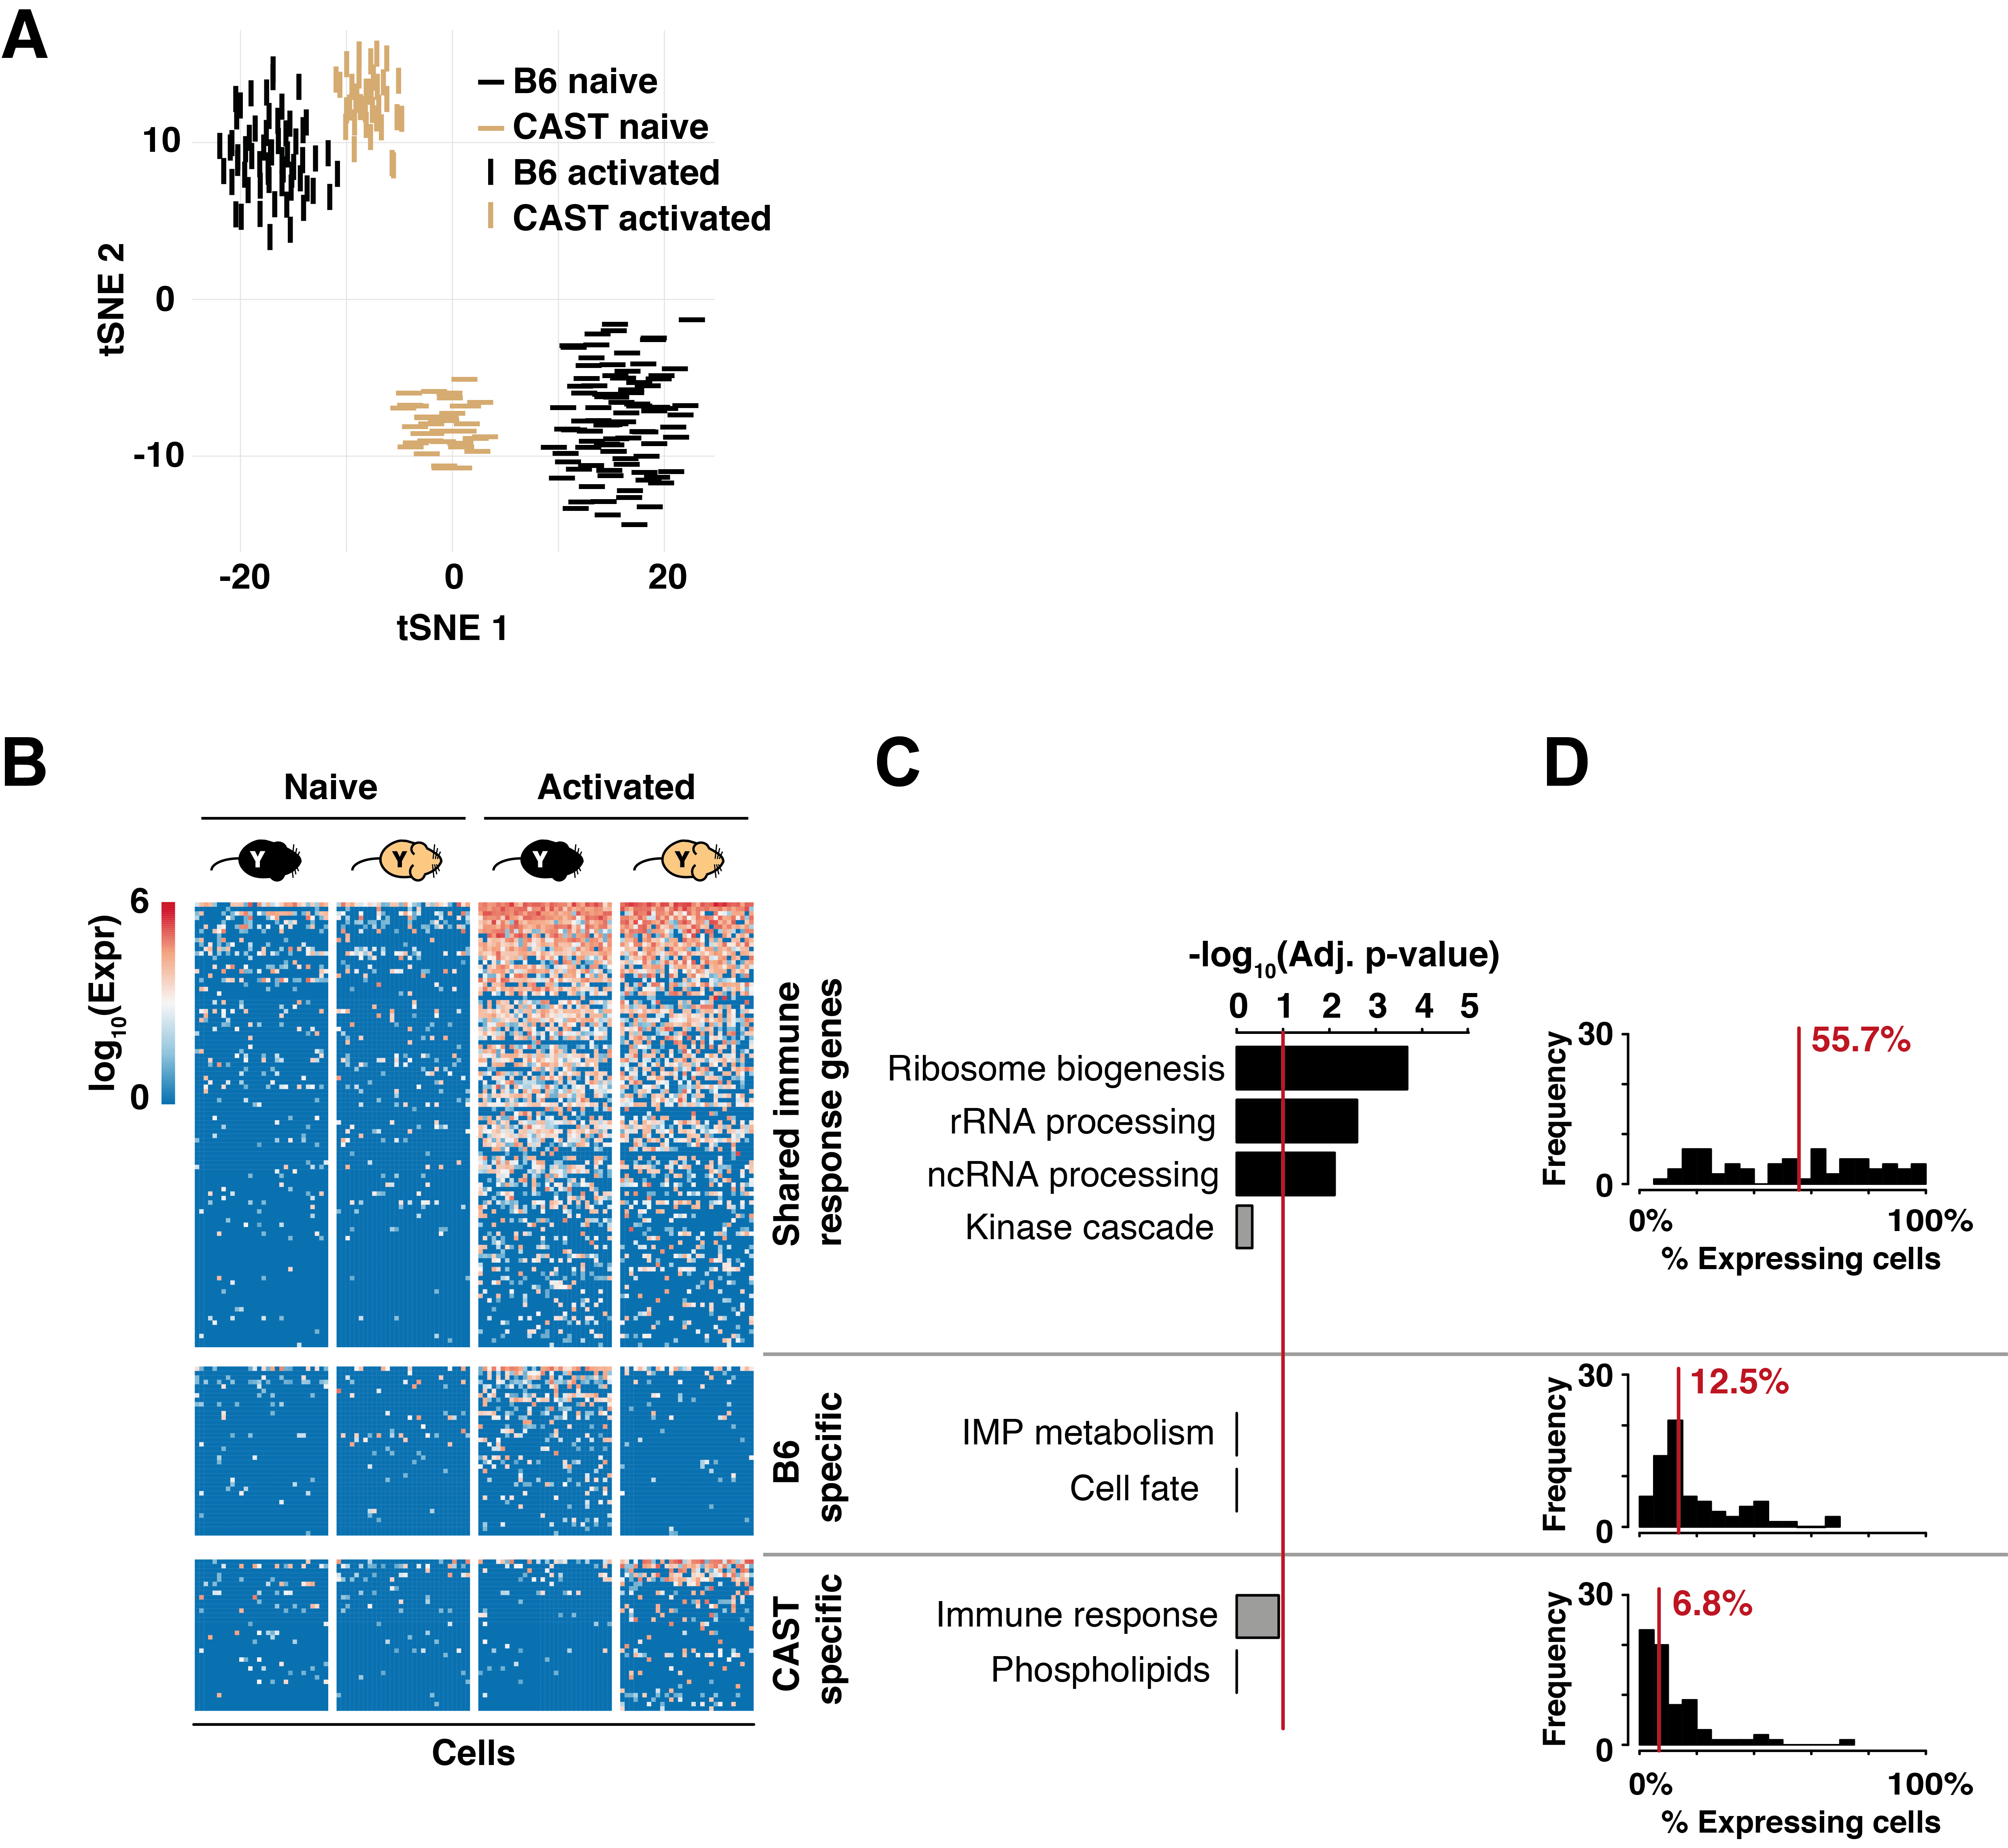
\includegraphics[width=\textwidth]{Fig_11.png}
\caption[X chromosome dynamics during spermatogenesis]{\textbf{X chromosome dynamics during spermatogenesis.} \\
\textbf{(A)} Schematic of sex chromosome sub-nuclear localisation through spermatogenesis, \textbf{(B)} For each cell, the ratio of mean expression of genes on Chr 9, Chr X and Chr Y to the mean expression of genes across all autosomes is represented as a boxplot for cells allocated to each developmental stage. SG – spermatogonia, M – metaphase, \textbf{(C)} Expression of all X chromosome genes (> 10 average counts) in bulk RNA-Seq data across the juvenile time course. Columns correspond to developmental stage and rows are ordered by the log$_2$ fold change between spermatocytes (stages before and including postnatal day (P) 20) and spermatids (stages after P20). Horizontal dashes indicate genes that are targets of \textit{Rnf8} (green) and \textit{Scml2} (blue) \citep{Adams2018}, \textbf{(D)} Average expression of spermatid-specific genes (panel (C)) per germ cell type. Columns are ordered by developmental stage and rows are ordered by peak gene expression through development. Multi-copy genes are highlighted in bold.}
\label{fig3:X_reactivation}
\end{figure}

\newpage

\section{Epigenetic mechanisms of X chromosome reactivation}

After identifying \emph{de novo} activated escape genes, we next profiled the epigenetic basis for such transcriptional dynamics. For this, we profiled the chromatin landscape in spermatocytes and spermatids using the newly developed CUT\&{}RUN protocol for low cell numbers \textbf{(Appendix \ref{appA.2})} \citep{Skene2018}. 

\subsection{CUT\&{}RUN to profile H3K4me3 and H3K9me3 marks}

In brief, from two individuals, we sorted spermatocytes and spermatids at P26 during the first wave of spermatogenesis \textbf{(Fig.~\ref{fig3:K9_global}A)}. At this stage, tubules contain spermatocytes close to the meiotic cell divisions and elongating spermatids. We assayed trimethylation of histone H3 on lysine 4 (H3K4me3) as a proxy for promoter activity, as well as repressive trimethylation of lysine 9 (H3K9me3). By profiling the enrichment of H3K9me3 across all chromosomes, we confirmed that the X chromosome has high levels of H3K9me3 in spermatids which has been previously shown \citep{Moretti2016, Greaves2006, Tachibana2007}. In addition, we now show that H3K9me3 accumulation begins earlier in meiosis, and indeed spermatocytes show enrichment of this repressive mark on the X chromosome \textbf{(Fig.~\ref{fig3:K9_global}B)}. \\

On autosomes, H3K9me3 is enriched in pericentromeric regions of constitutive heterochromatin \citep{Peters2001}. To assay the distribution of read pairs across whole chromosomes, we binned reads in 1kb windows across the chromosome. Next, we calculated the cumulative sum across 10,000 randomly sampled bins starting at windows with highest H3K9me3 enrichment. This measure indicates whether each window contains equal enrichment (slope is similar across the curve) or if some windows are enriched for the mark (slope decreases across the curve). As seen in \textbf{Fig.~\ref{fig3:K9_global}D}, the H3K9me3 enrichment appears to be homogeneously distributed across the X chromosome while, for example, the enrichment of the H3K9me3 mark on chromosome 9 is a lot more heterogeneous. \\

Nevertheless, when merging the 1000 windows with highest H3K9me3 enrichment, we detected broad regions showing particularly high levels of H3K9me3 scattered across the X chromosome \textbf{(Fig.~\ref{fig3:K9_global}C)}. Among the merged regions with highest H3K9me3 enrichment, we detect the promoter of \textit{Akap4}, a well-known escape gene. This discovery prompted us to profile the chromatin dynamics of active and repressive marks at promoters of \emph{de novo} escape genes (\emph{spermatid-specific genes}) versus the promoters of all other expressed X-chromosome genes (\emph{non-spermatid specific genes}) \textbf{(Fig.~\ref{fig3:X_reactivation}C)}.

\begin{figure}[!h]
\centering
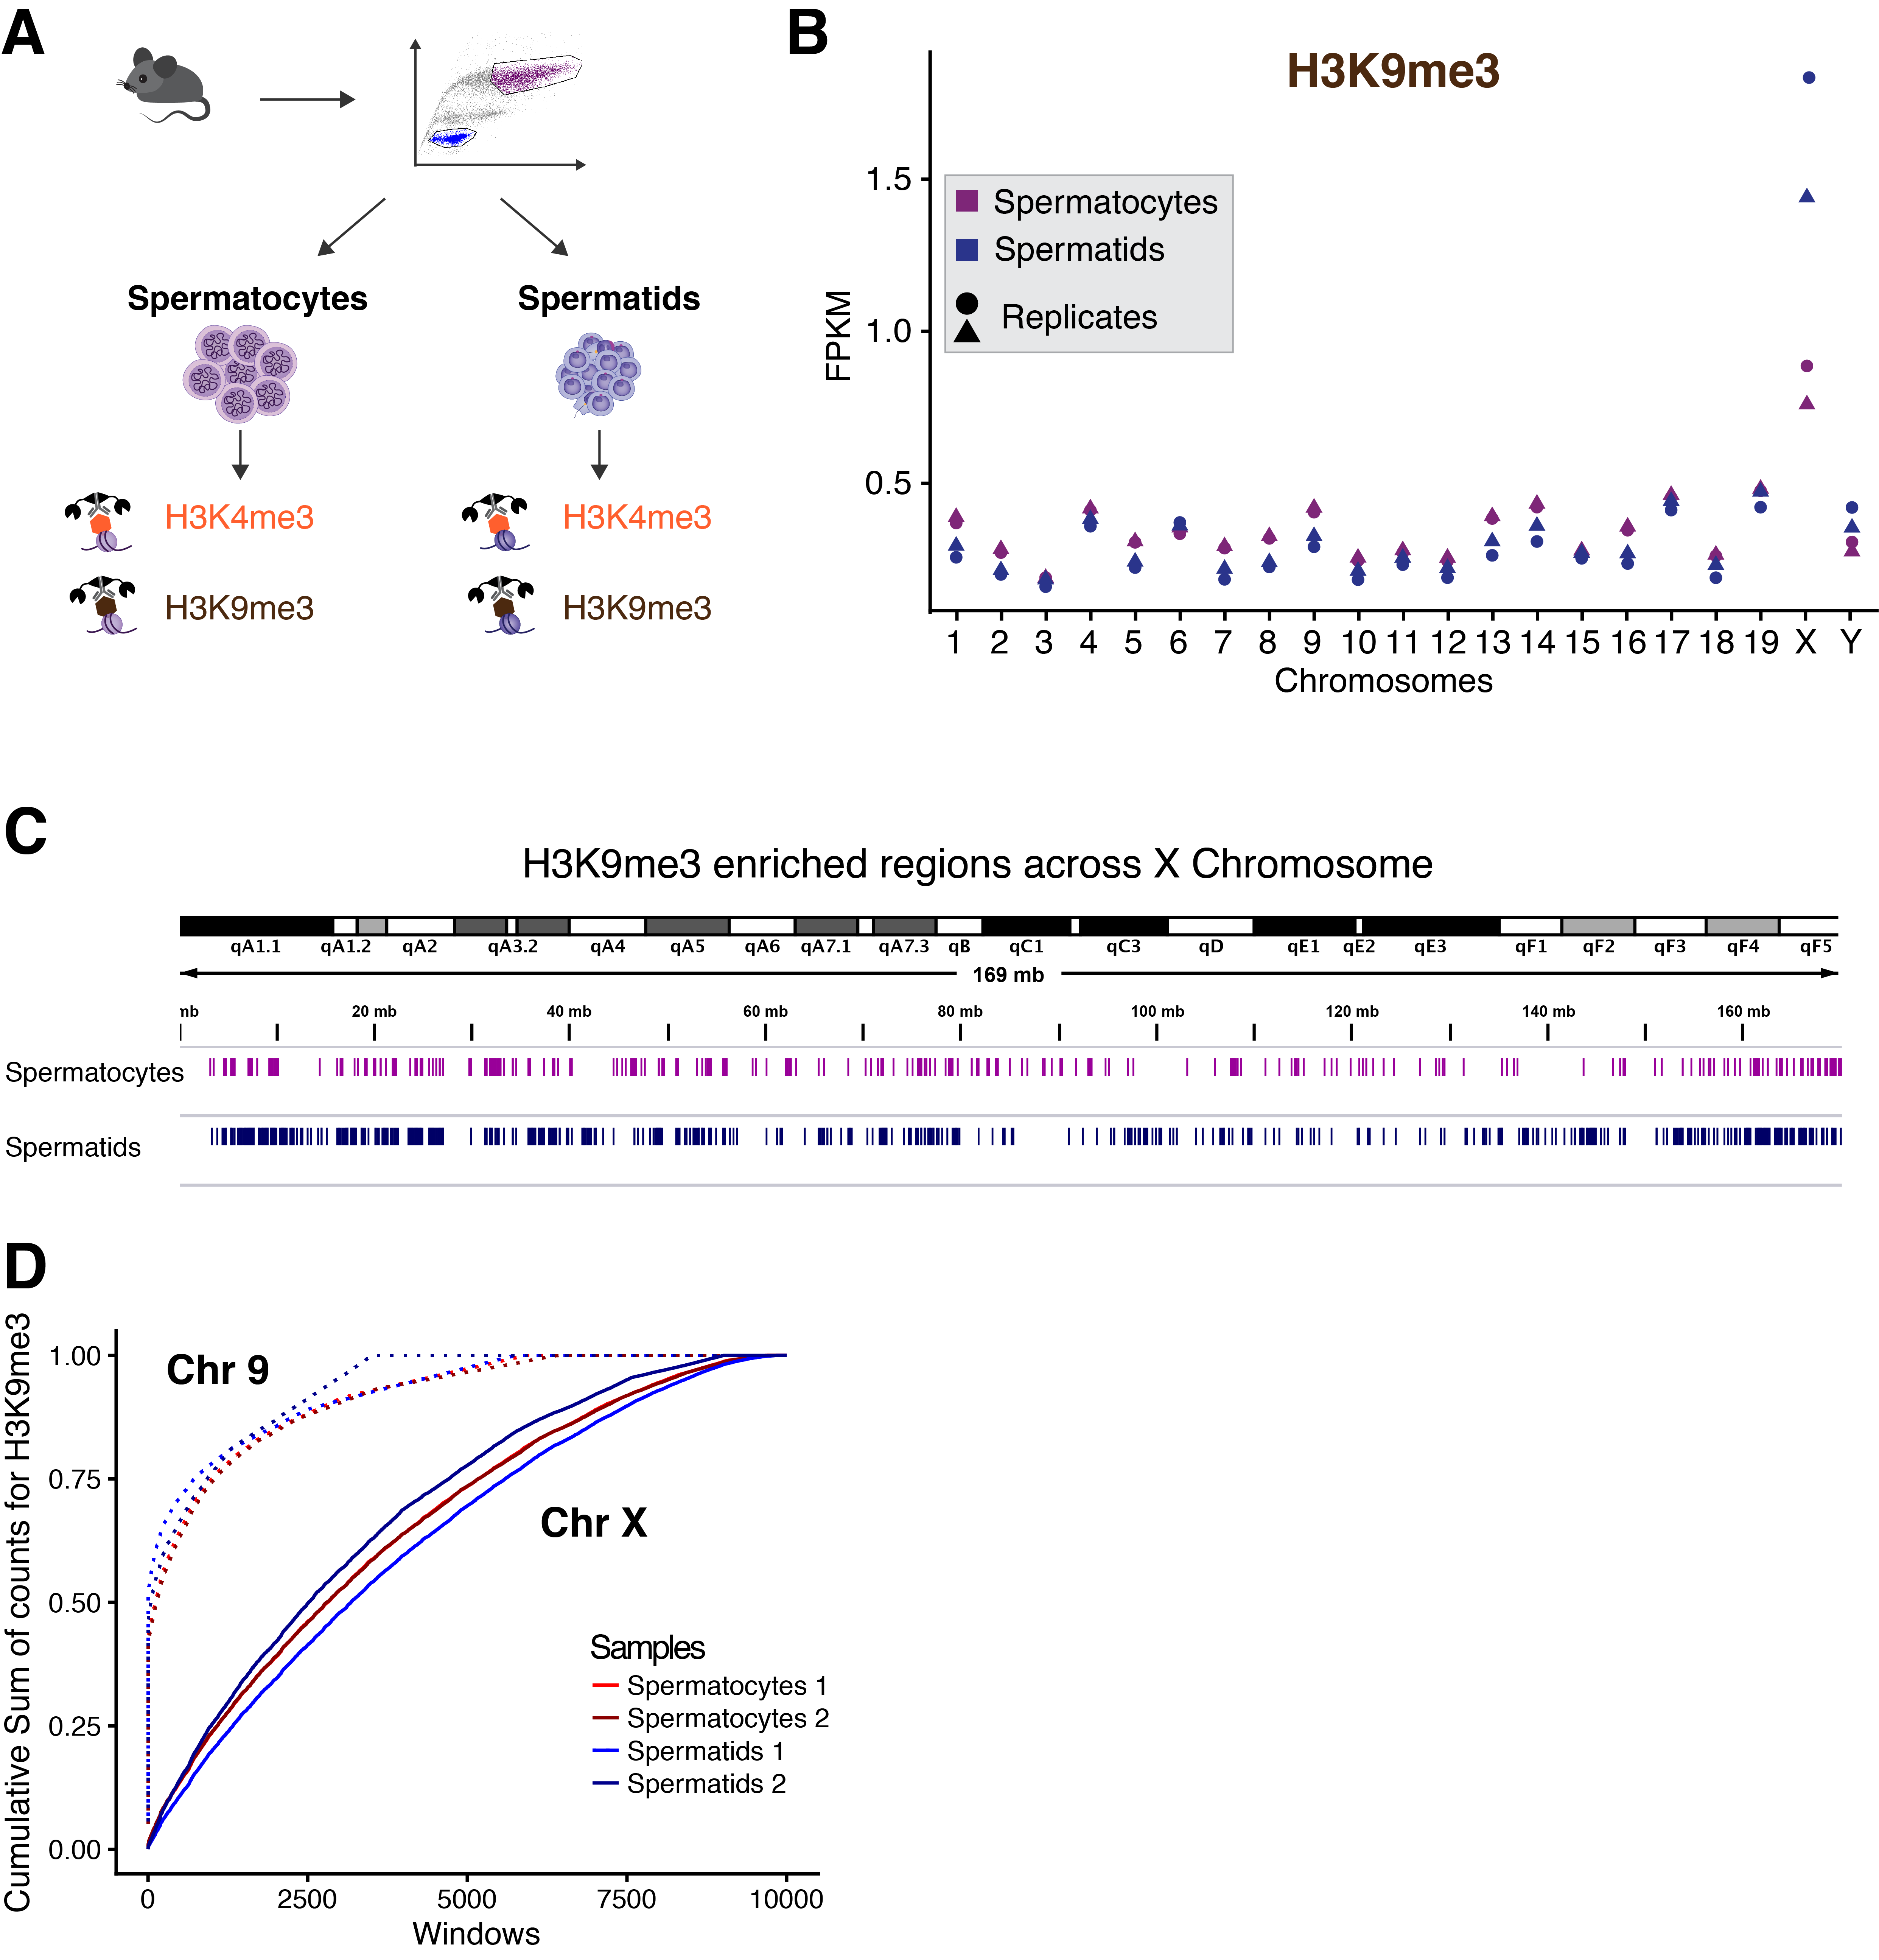
\includegraphics[width=\textwidth]{Fig_12.png}
\caption[Chromatin profiling in spermatocytes and spermatids]{\textbf{Chromatin profiling in spermatocytes and spermatids.} \\
\textbf{(A)} Spermatocytes and spermatids were isolated from the same individual using FACS and profiled using H3K4me3 (active mark) and H3K9me3 (repressive mark) using CUT\&{}RUN, \textbf{(B)} Number of H3K9me3 Fragments Per Kilobase per Million (FPKM) for each chromosome. Pink: spermatocytes, blue: spermatids. Shape corresponds to biological replicate, \textbf{(C)} The top 1000 windows with highest H3K9me3 signal (1000 bp width, CPM) were merged using a tolerance of 1500 bp. Representative tracks of one replicate in spermatocytes and one replicate in spermatids are shown, \textbf{(D)} Cumulative summed counts per million across 10000 randomly sampled windows (1000 bp width) visualizing the distribution of the H3K9me3 signal across chromosome 9 (dashed line) and chromosome X (solid line).}
\label{fig3:K9_global}
\end{figure}

\newpage

\subsection{Targeted silencing of spermatid-specific escape genes}

Here, we profiled the enrichment for H3K4me3 and H3K9me3 marks at promoters of spermatid-specific escape genes and all other X-linked genes in spermatides and spermatocytes. As a measure for enrichment, we calculated the Counts Per Million (CPM) for paired reads per promoter. In spermatocytes, spermatid-specific genes showed lower enrichment in H3K4me3 than non-spermatid specific genes (Wilcoxon-Mann-Whitney: p-value < 2.2x10$^{-16}$) \textbf{(Fig.~\ref{fig3:K9_K4_targeted}A, left panel)}. In contrast, spermatid-specific genes have on average elevated H3K4me3 in spermatids, as expected based on their increased expression level compared to spermatocytes \textbf{(Fig.~\ref{fig3:K9_K4_targeted}A, right panel)}. \\


When examining the deposition of H3K9me3 on the promoters of X-linked genes, we detected a strong enrichment in spermatid-specific escape genes in spermatocytes (Wilcoxon-Mann-Whitney: p-value < 3.7x10$^{-11}$) \textbf{(Fig.~\ref{fig3:K9_K4_targeted}B, left panel)}. This pattern indicates that spermatid-specific genes are more strongly repressed in spermatocytes. Due to the strong enrichment of H3K9me3 on the post-meiotic X chromosome, we detect similar H3K9me3 enrichment in promoters for both, spermatid-specific and non-specific X-linked genes \textbf{(Fig.~\ref{fig3:K9_K4_targeted}B, right panel)}.\\

Our results describe the precise epigenetic changes associated with escape gene activation in post-meiotic cells. These dynamics are exemplified by the chromatin remodelling that occurs around \textit{Akap4} and \textit{Cypt1}, both of which are well-studied spermatid-specific genes \textbf{(Fig.~\ref{fig3:K9_K4_targeted}C)}. The promoters of these genes have high levels of H3K9me3 in spermatocytes, which decreases in spermatids, while H3K4me3 levels are strongly increased. This targeted repression of a subset of X-linked escape genes could indicate a mechanism to repress otherwise lethal genes in spermatocytes that are later on needed in spermatid development. Examples of spermatocyte-lethal genes involved in spermatid development are two Y chromosome encoded genes: zinc finger protein Y-linked (\textit{Zfy}) 1 and 2 \citep{Royo2010}.

\newpage

\begin{figure}[!h]
\centering
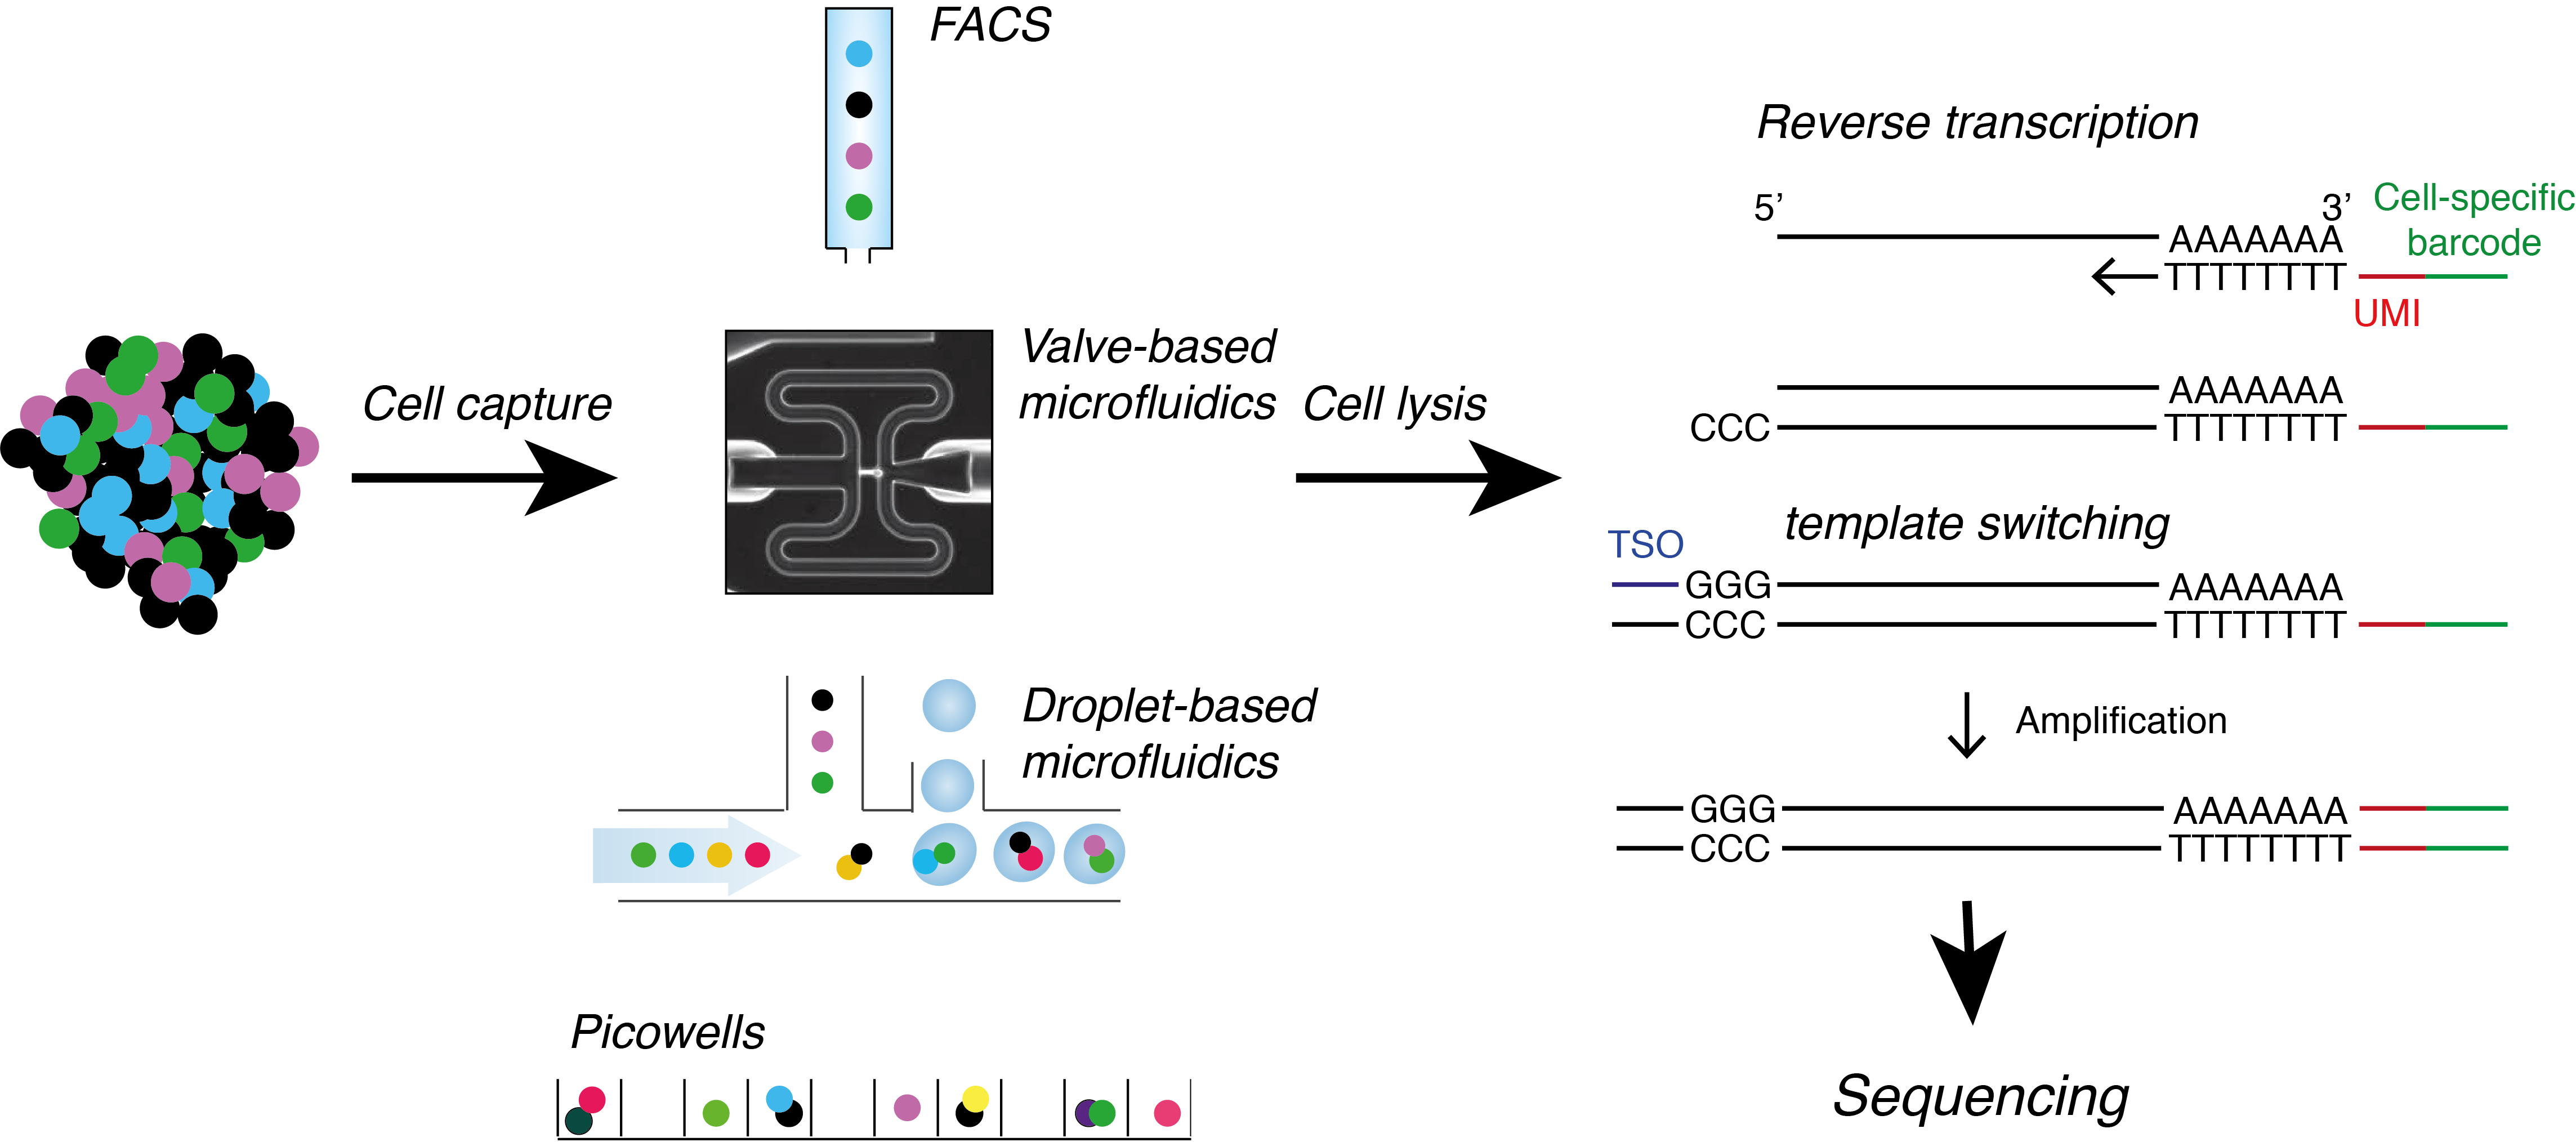
\includegraphics[width=\textwidth]{Fig_13.png}
\caption[Targeted repression of spermatid-specifc escape genes in spermatocytes]{\textbf{Targeted repression of spermatid-specifc escape genes in spermatocytes.} \\
\textbf{(A)} and \textbf{(B)} Boxplot of H3K4me3 (A) and H3K9me3 (B) Counts Per Million (CPM) in promoter regions of spermatid specific (n=127) and non-spermatid specific (n=617) genes for spermatocytes (left) and spermatids (right).  \# indicates statistical significance (Wilcoxon-Mann-Whitney: p-value < 1x10$^{-10}$), n.s. – not significant, 
\textbf{(C)} Genome tracks of H3K4me3 and H3K9me3 for two representative spermatid-specific genes (\textit{Akap4} and \textit{Cypt1}) for spermatocytes (left) and spermatids (right). Reads were scaled by library size. The genomic location of these genes is indicated below the tracks where exons are labelled as blocks and the directionality of transcription is shown by arrows.}
\label{fig3:K9_K4_targeted}
\end{figure}

\newpage

\section{Measuring changes in variability over pseudo-time}

As described above, spermatogenesis is a unidirectional and continuous differentiation process coupled to a complex system of developmental steps. I next asked whether this differentiation process is coupled to changes in transcriptional variability. In mouse hematopoietic cell differentiation, cell-to-cell diversity increases at critical state transitions where cell fate decisions are made \citep{Mojtahedi2016}. A similar effect was detected in chicken erythroid progenitor cells where the Shannon entropy is highest directly at the point of fate commitment and declines upon the irreversible commitment to differentiation \cite{Richard2016}. In the previous chapter, we have demonstrated that transcriptional variability shows dynamic changes during CD4\plus{} T cell differentiation with high variability being observed at a possible early commitment point and a decrease in variability upon proliferation. In this section, I applied the regression BASiCS model which was developed in the previous chapter to study changes in transcriptional variability over the time-course of spermatogenesis. More specifically, I profiled changes in variability for individual genes during spermiogenesis, the differentiation process that directly follows meiosis (see \textbf{Section \ref{sec3:spermiogenesis}}). As described above, spermiogenesis is a differentiation process that involves an extensive remodelling of the chromatin with transcriptional shut-down occurring at around spermatid stage S10. Modelling changes in expression over a differentiation time-course is done by ordering transcriptional profiles of individual cells along their so called \emph{pseudo-time}. Different methods have been proposed to perform this ordering based on minimum spanning trees \citep{Trapnell2014} and nearest-neighbour graphs \cite{Setty2016}, Gaussian Processes \citep{Reid2016a, Campbell2016b} and diffusion maps \citep{Haghverdi2016}. Once the pseudo-temporal ordering is determined, genes which change in expression over pseudo-time can be found by fitting a generalized linear model to the expression counts and performing a likelihood ratio test against a null model with no pseudo-time dependence \citep{Trapnell2014}. Profiling changes in variability is more complicated as single-cell measures of variability are not available. 

\subsection{Using BASiCS on continuous data}

Here, I use BASiCS to estimate residual over-dispersion parameters for homogeneous cell populations along the differentiation time-course. Different approaches of identifying homogeneous populations exist. First, ordered cells can be split into populations of equal size (e.g.~200 cells per group). This approach produces heterogeneous cell populations when cell state transitions occur within the population. I therefore rely on the clustering performed in \textbf{Section \ref{sec3:clustering}} which splits the full cell population along the differentiation trajectory. For each cluster from S1 to S14, the regression BASiCS model was run for 40,000 iterations with 20,000 iterations burn-in and a thinning value of 20. 

\newpage

For each gene in each of the 14 spermatid populations, BASiCS generates a posterior distribution estimating the residual over-dispersion parameter in form of an MCMC chain \textbf{(Fig.~\ref{fig3:variability_schematic}A)}. These measures are independent of mean expression (see previous chapter) and can therefore be used to study changes in variability which are not confounded by changes in mean expression throughout the differentiation of sperm. To profile and test temporal changes of transcriptional variability during spermiogenesis, I choose two approaches. \\

First, I used iterative fitting of a linear regression between the residual over-dispersion parameters and the progression of spermiogenesis to find linear changes in variability. For this, I selected spermatids from stages S1 to S9 prior to transcriptional shut-down. Transcriptional changes after S10 are only due to degradation of mRNA and I assume that linear changes in variability occur before S10. In more detail, for each MCMC iteration, I fit a linear regression between the current samples of $\epsilon_i$ against the cluster label \textbf{(Fig.~\ref{fig3:variability_schematic}B)}. This fitting is performed for each gene individually and generates a \emph{post hoc} distribution of the intercept and the slope regression coefficient that captures uncertainty in the regression fit. Focusing on the slope coefficient, I can compute the posterior tail probability of the slope coefficient being different from 0. If the posterior tail probability is larger than a threshold (e.g.~80\%), I consider the transcriptional variability of this gene to be either positively or negatively associated with temporal ordering depending on the sign of the median slope coefficient \textbf{(Fig.~\ref{fig3:variability_schematic}B)}. Similar to differential testing described in the previous chapter, the probability threshold is determined by fixing the expected false discovery rate to 10\%. A similar testing can be done for the slope coefficient when fitting a linear model between the group wise mean expression parameter $\log(\mu_i)$ and the group labels.\\

Secondly, to detect non-linear patterns of changes in transcriptional variability, I perform clustering on the gene-specific variability profiles across spermatid populations S1-S14. Similar approaches have been chosen to find patterns of genes expression across pseudo-time. Common patterns for changes in expression levels include immediate, transient and gradual up- or down-regulation \citep{Trapnell2014}. When profiling changes in variability over the time-course of differentiation these clustered profiles can indicate similarly strong or weak transcriptional regulation or similar expression rates \textbf{(Fig.~\ref{fig3:variability_schematic}C)}.

\newpage

\begin{figure}[!h]
\centering
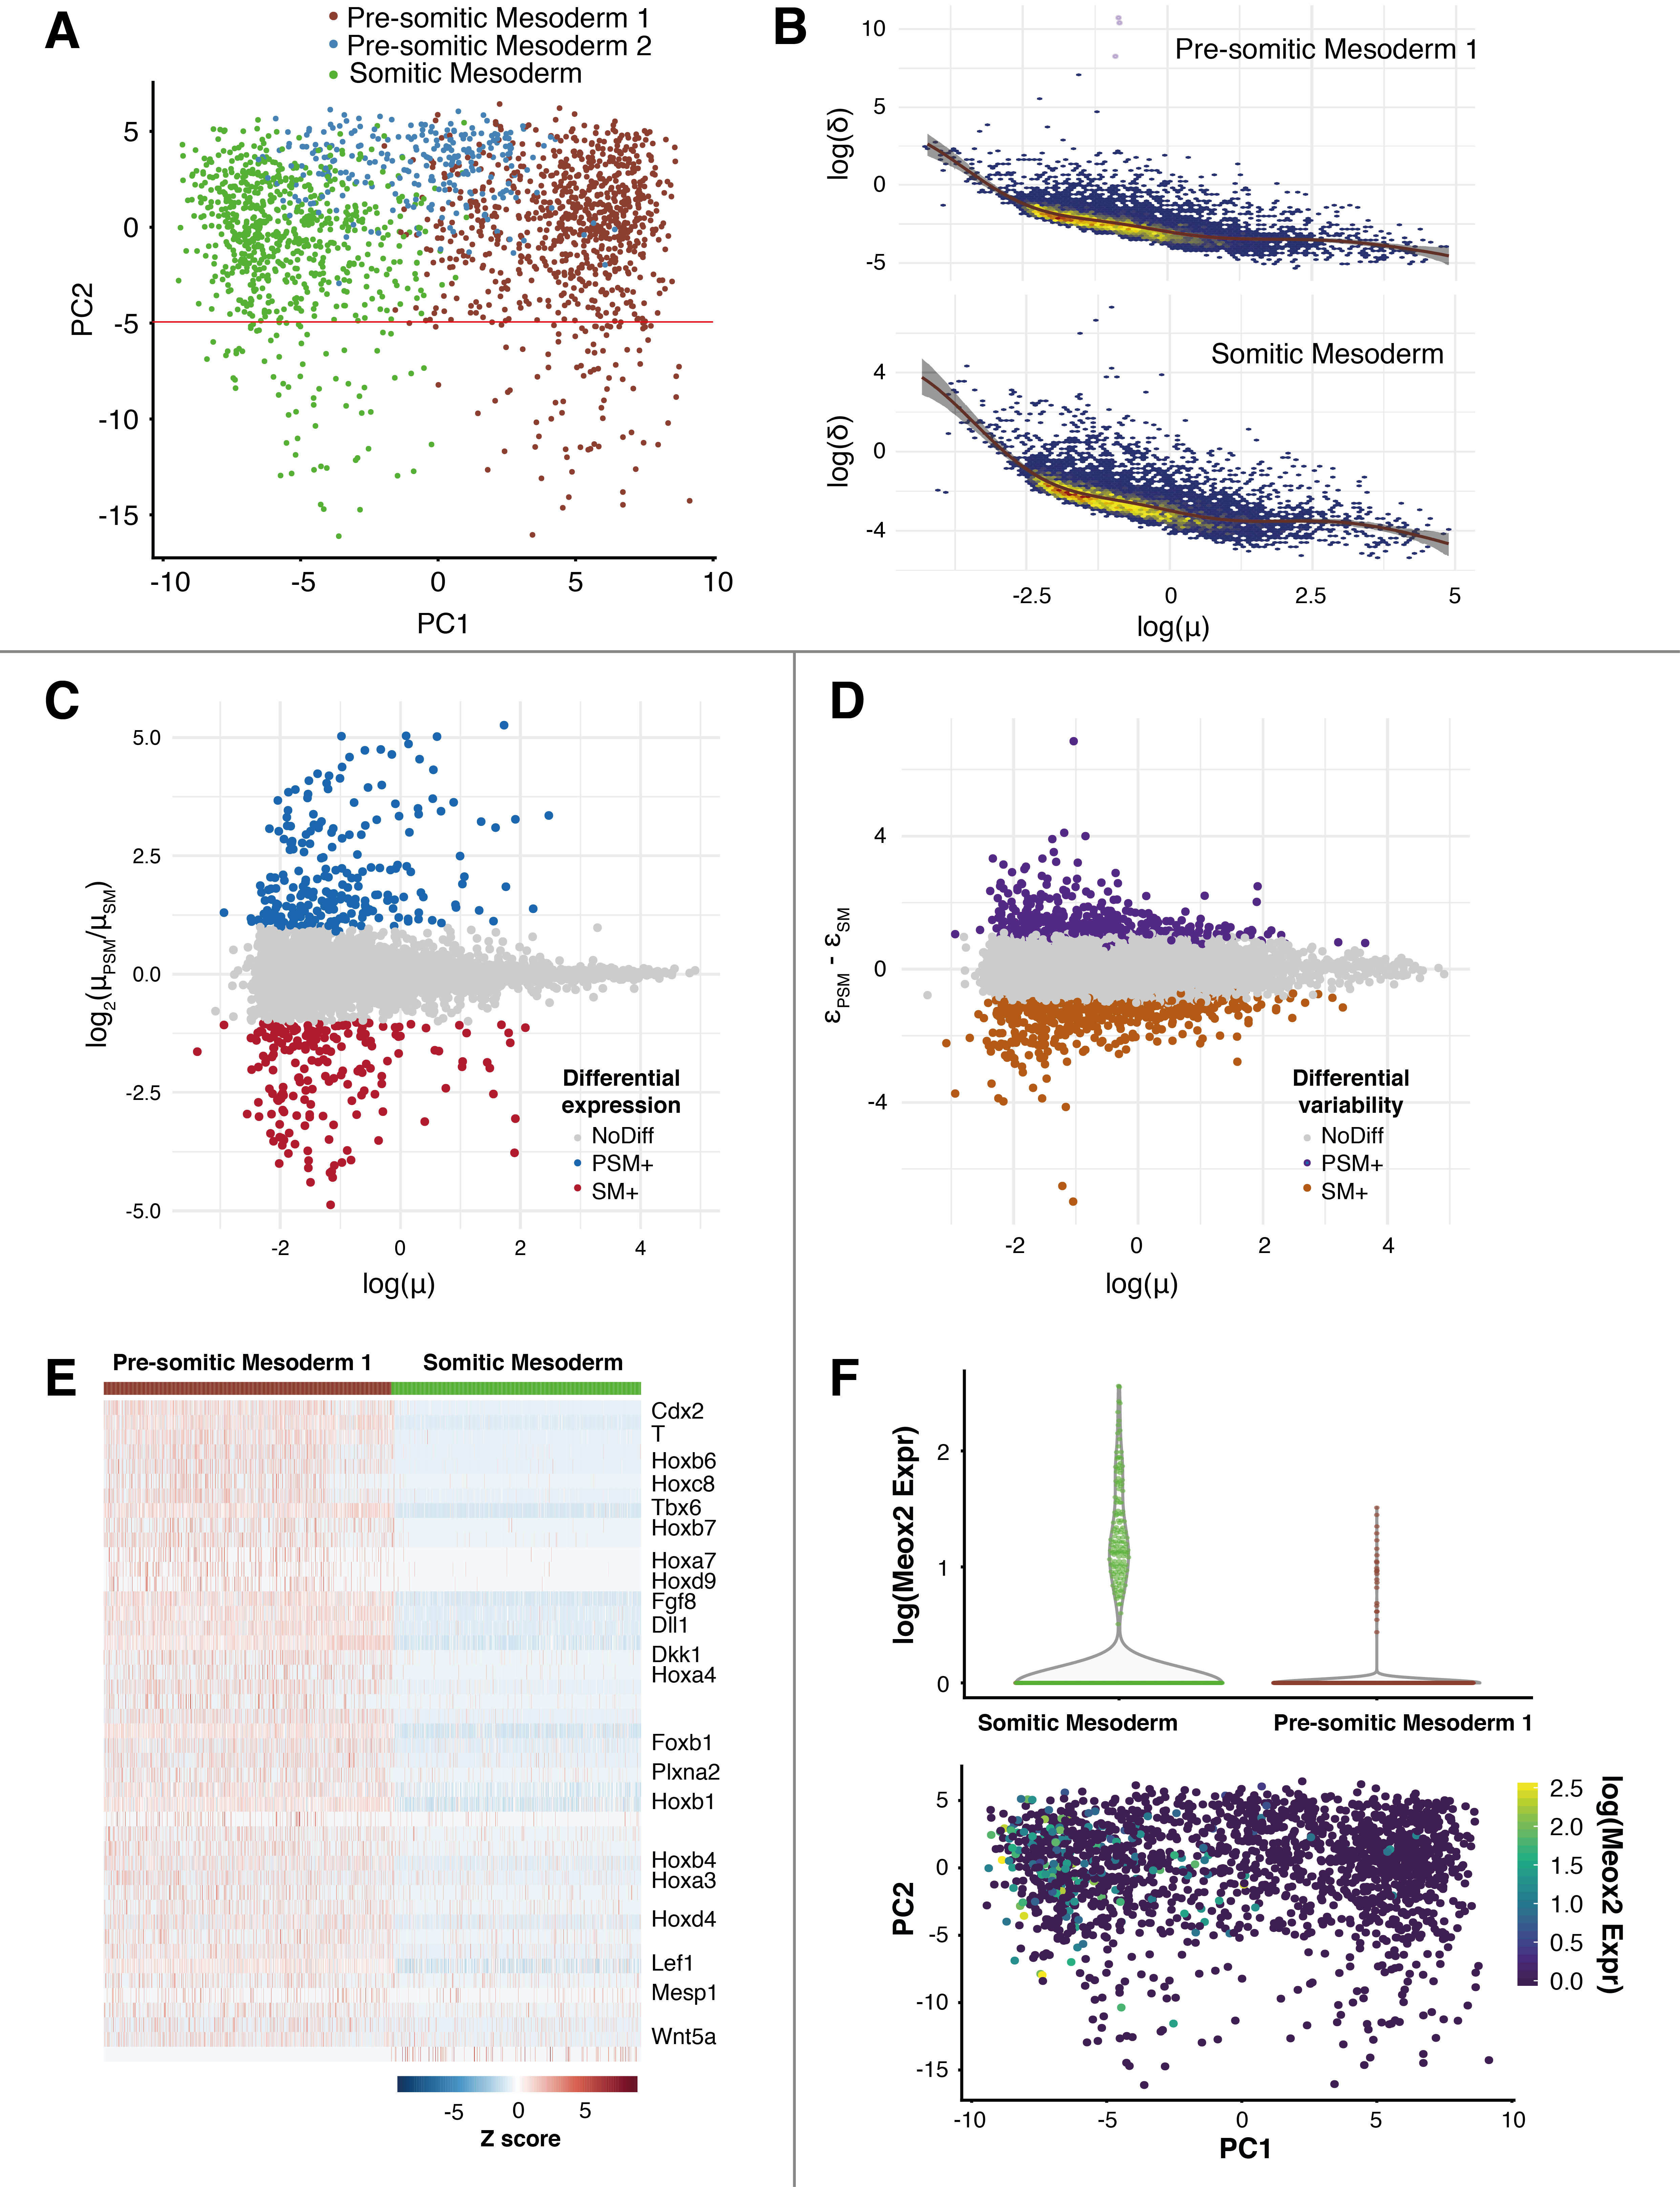
\includegraphics[width=0.8\textwidth]{Fig_14.png}
\caption[Detecting changes in variability over pseudo-time]{\textbf{Detecting changes in variability over pseudo-time.}\\
\textbf{(A)} For each group of spermatid, BASiCS  generates a posterior distribution of residual over-dispersion parameters $\epsilon_i$. Cell groups can be ordered based on their pseudo-time (upper panel). Lower panels indicate the MCMC chain for gene-specific $\epsilon_i$ per group (A, B, ..., X), \textbf{(B)} For each iteration of the MCMC (1,...,n), a linear regression was fit between the current samples of $\epsilon_i$ against the group labels for spermatids (S) 1-9. This approach generates a \emph{post hoc} distribution of the slope coefficient $\beta_1$ (lower panels). The distribution is used to calculate the posterior probability of observing $\beta_1\neq0$, \textbf{(C)} Clustering was performed on variability profiles across spermatid populations S1 to S14. A smooth regression (loess) was fit to $\epsilon_i$'s of the genes within each cluster. Genes that quickly decrease in variability (left panel), increase then decrease in variability (middle panel) or quickly increase in variability (right panel) can be identified.}
\label{fig3:variability_schematic}
\end{figure}

\newpage

\subsection{Finding continuous changes in variability by linear model fitting}

To detect single genes that continuously increase of decrease in variability, I fit a linear regression to each iteration of the MCMCs sampling $\epsilon_i$ or $\mu_i$ \emph{versus} the group labels \textbf{(Fig.~\ref{fig3:variability_schematic}B)}. The posterior distributions of the slope coefficient were used to categorise genes based on their transcription dynamics along the differentiation time-course (middle panel in \textbf{Fig.~\ref{fig3:linear_variability}}). These categories include: 

\begin{itemize}
\itemsep0em 
\item Increase in mean expression, no change in variability
\item Increase in mean expression, increase in variability
\item Increase in mean expression, decrease in variability
\item Decrease in mean expression, no change in variability
\item Decrease in mean expression, increase in variability
\item Decrease in mean expression, decrease in variability
\item No change in mean expression, no change in variability
\item No change in mean expression, increase in variability
\item No change in mean expression, decrease in variability
\end{itemize}

This approach leads to the detection of few genes that significantly change in variability over the differentiation time-course in a linear fashion while the majority of genes change only in mean expression. One hypothesis is that sperm maturation is a tightly regulated progress where the majority of genes follow a clear transcriptional pattern. Such a process contrasts other differentiation programmes such as hematopoiesis where branching events occur and the whole cell population expands in transcriptional variability to find new attractor states \citep{Mojtahedi2016}. To visualize changes in transcriptional variability, I selected representative genes from four categories: (i) Increase in mean expression, increase in variability, (ii) Increase in mean expression, decrease in variability (iii) Decrease in mean expression, increase in variability, (iv) Decrease in mean expression, decrease in variability (see inlets in \textbf{Fig.~\ref{fig3:linear_variability}}). Interestingly, \textit{Tsga8}, one of the most rapidly evolving X-linked genes, shows a strong increase in expression and a clear decrease in transcriptional variability. \emph{Tsga8} has been reported to be involved in hybrid sterility where F$_1$ crosses of mice form different strains are unable to reproduce. This effect might be due to the strong divergence of the \emph{Tsga8} sequence between species \citep{Good2011}. A tight regulation of its expression during spermiogenesis can therefore further control the phenotypic effect in F$_1$ animals.

\newpage

\begin{figure}[!h]
\centering
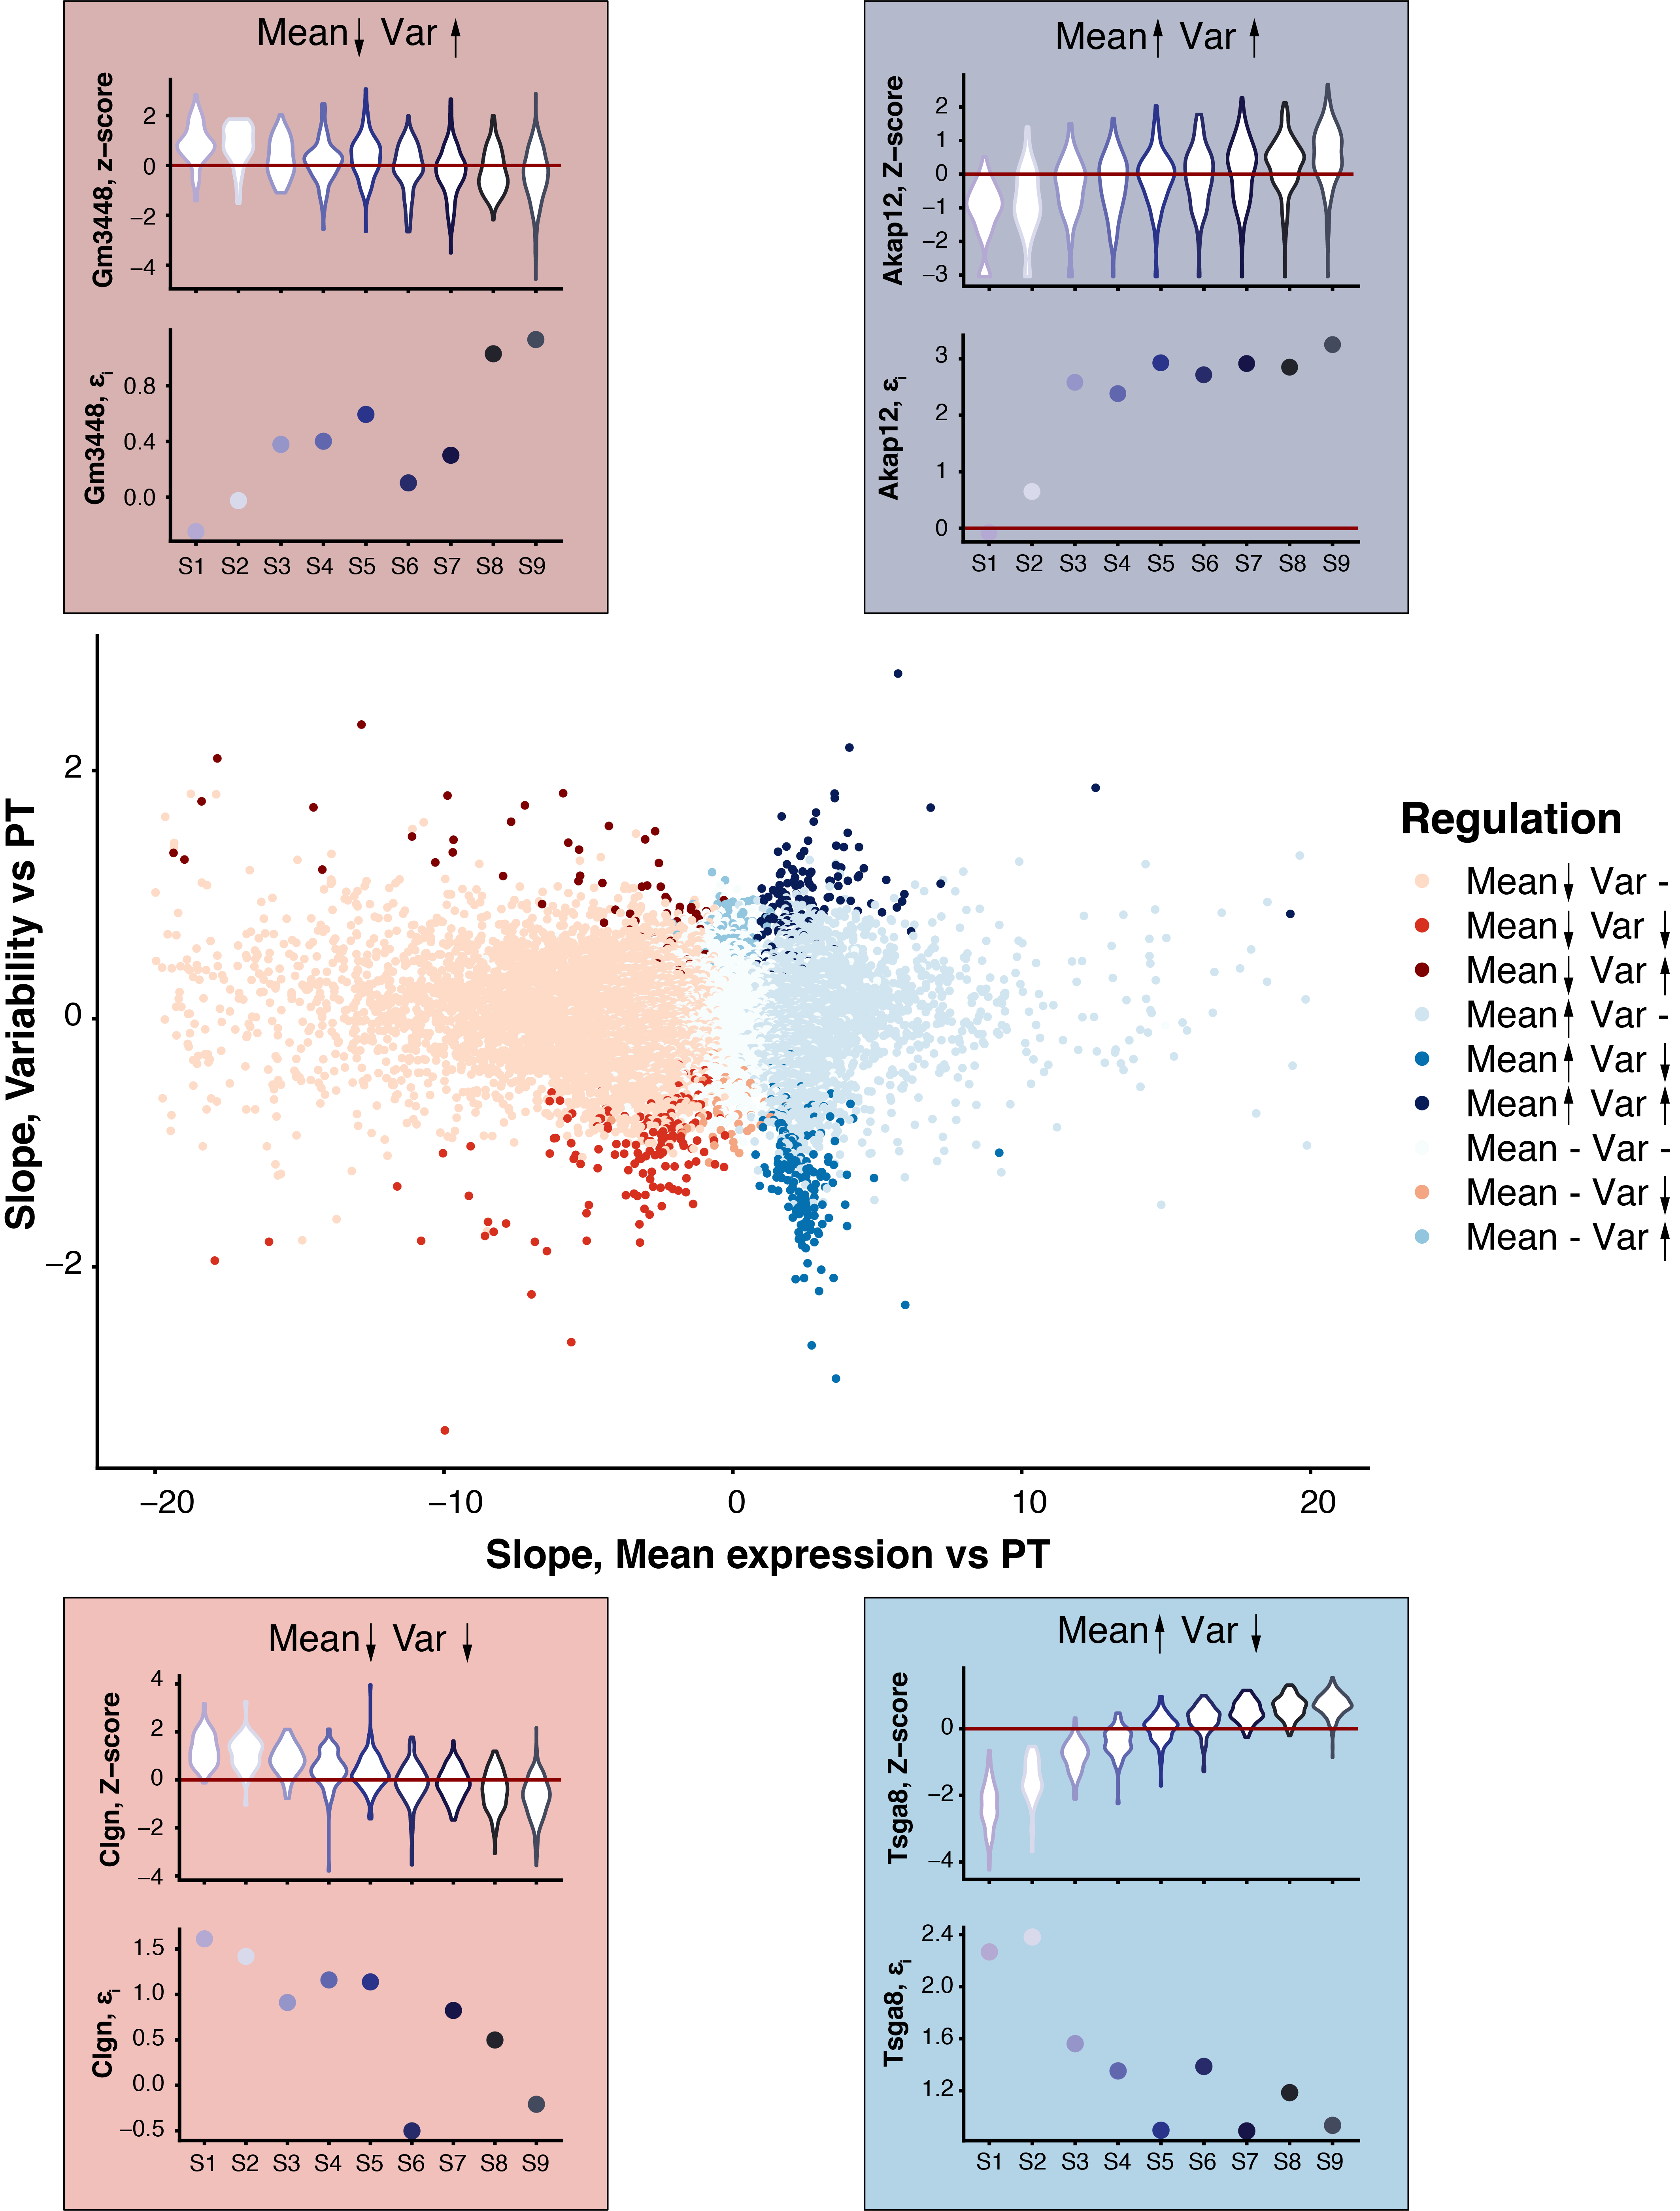
\includegraphics[width=0.8\textwidth]{Fig_15.png}
\caption[Linear changes in variability over spermiogenesis]{\textbf{Linear changes in variability over spermiogenesis.}\\
Linear models were fit between the residual over-dispersion parameter $\epsilon_i$ or the mean expression parameter $\mu_i$ and the groups labels (S) 1-14 for each iteration of the MCMC. Median posterior estimates of the slope parameter of the variability fit were plotted against the slope parameter of the mean expression fit. each dot represents a single gene. Genese are coloured based on their regulation (legend). Plot inlets indicated the Z score scaled normalized expression (upper panel) and the group-wise residual over-dispersion estimates $\epsilon_i$ (lower panels) of representative genes for four categories.}
\label{fig3:linear_variability}
\end{figure}

\newpage

\subsection{Clustering of variability profiles}

To identify non-linear patterns across all genes, I first ordered variability profiles based on their peak in variability \textbf{(Fig.~\ref{fig3:variability_clustering}A)}. Here, variability profiles are represented by the median residual over-dispersion parameter $\epsilon_i$  ordered from S1 to S14. Most variability profiles showed highest variability in specifically one group while also other patterns of variability are detectable. \\

To identify the major patterns of variability across the full range of spermiogenesis, I performed k-means clustering across all variability profiles. In this case, I had to select the expected number of clusters. Due to the fact that most genes showed peak variability in exactly one group, I selected $\text{k}=20$ to detect patterns other than peaks in single groups. After clustering, I detect a variety of variability patterns ranging from high variability in early spermiogenesis to high variability at later stages \textbf{(Fig.~\ref{fig3:variability_clustering}B)}. Most interestingly, I observed patterns that show gradual increase in variability until around spermatid stage S9 and decrease afterwards \textbf{(Fig.~\ref{fig3:variability_clustering}B, middle panel)}. \\

The group with peak variability at around S9 consists of all transition proteins (\textit{Tnp1}, \textit{Tnp2}) and protamins (\textit{Prm1}, \textit{Prm2}, \textit{Prm3}). When visualizing the expression patterns of \textit{Prm1}, I detect a quick shift in expression within cells from S9 \textbf{(Fig.~\ref{fig3:variability_clustering}C, middle panel)}. Similarly, genes that show highest variability at later stages during spermiogenesis \textbf{(Fig.~\ref{fig3:variability_clustering}B, second to last panel)} show a quick transcriptional decline after transcriptional shut-down (e.g.~ \emph{Tekt4}, \textbf{Fig.~\ref{fig3:variability_clustering}B}). \\

These results indicate that the changes in expression associated to the trajectory of pseudo-time are additional confounding factors when quantifying transcriptional variability. Similar to removing the confounding between mean expression and variability, a regression approach can be chosen to correct variability measures based on the correlation between expression and pseudo-time. 



\newpage

\begin{figure}[!h]
\centering
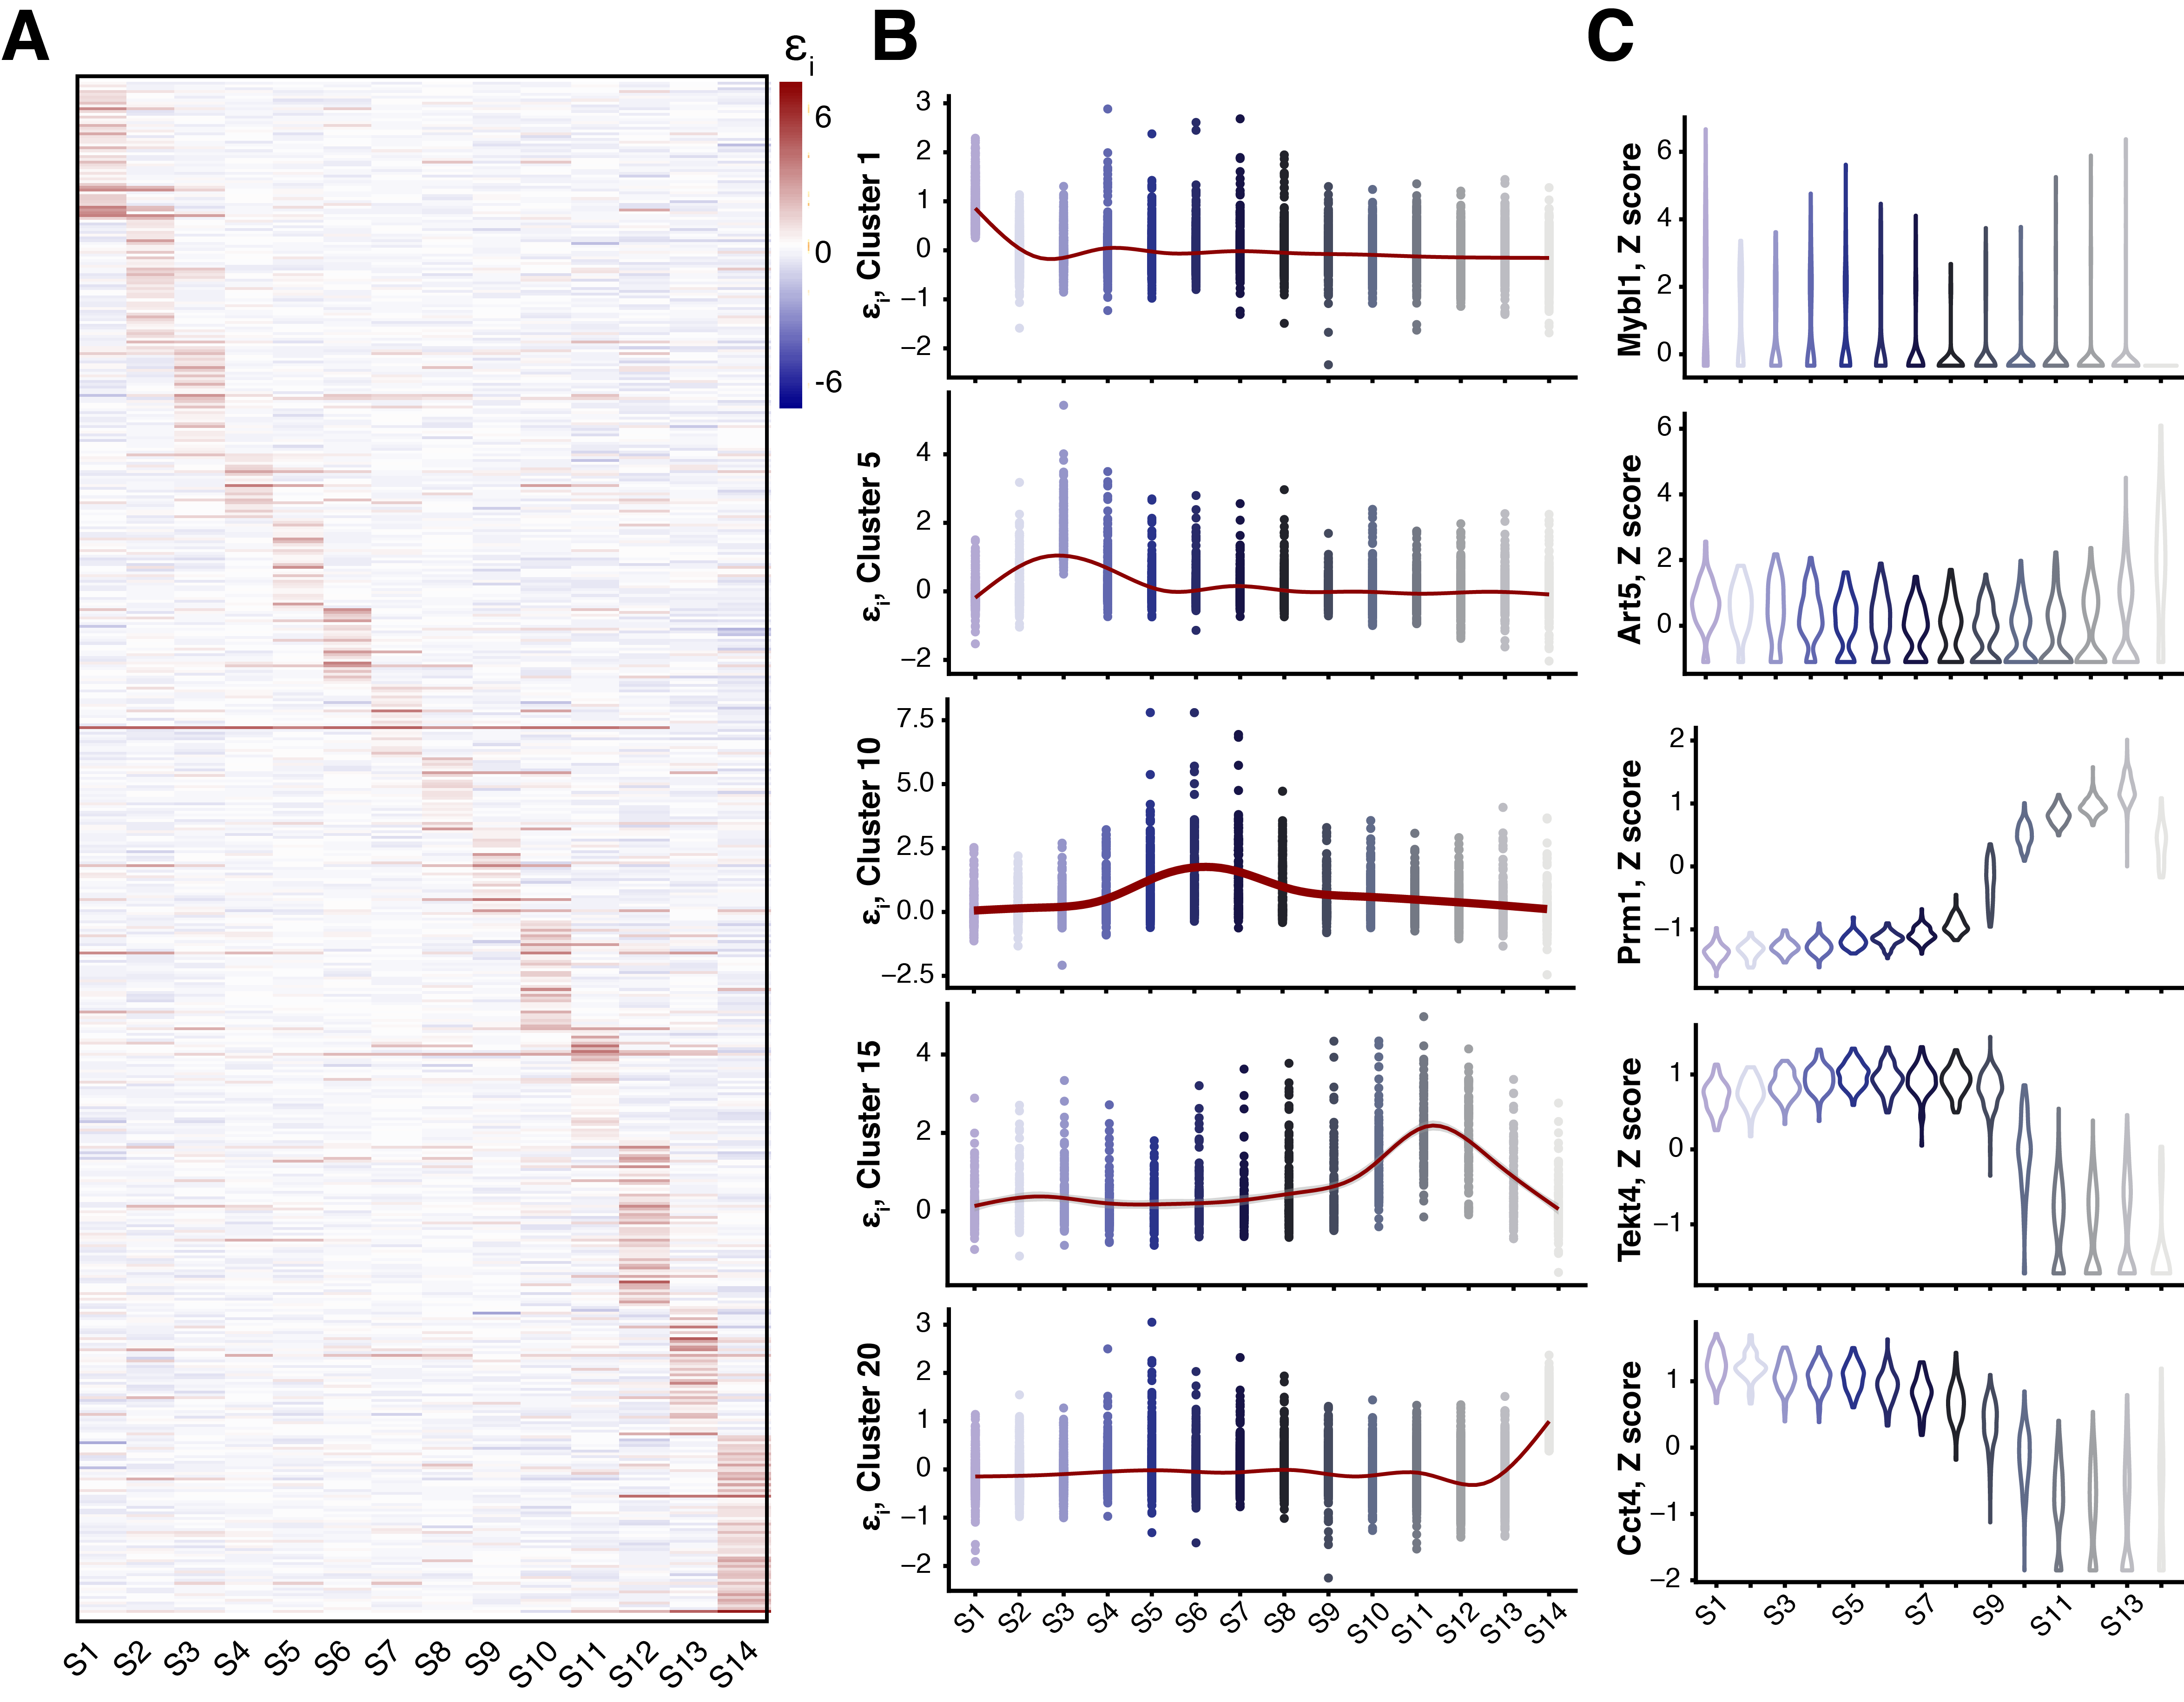
\includegraphics[width=\textwidth]{Fig_16.png}
\caption[Clustering of variability profiles]{\textbf{Clustering of variability profiles.}\\
\textbf{(A)} Variability profiles (median of the $\epsilon_i$ estimates ordered by developmental progression) were ordered based on their maximum $\epsilon_i$ starting in S1 spermatids, \textbf{(B)} Variability profiles were clustered using k-means with $\text{k}=20$. 5 representative patterns of variability are displayed ranging from highest variability in round spermatids to highest variability in elongating spermatids, \textbf{(C)} Z score scaled, normalized expression of example genes per variability pattern taken from (B) are displayed in form of boxplots.}
\label{fig3:variability_clustering}
\end{figure}

\newpage
%!TEX root = ../chapter3.tex
%******************************
%	 Discussion 
%*****************************

\section{Discussion}

The testes are among the most proliferative tissues in the adult body and ensure fertility via the continuous production of millions of sperm per day. Most developmental differentiation processes require the profiling of cellular populations at several time points \citep{Kernfeld2018, Scialdone2016, Wagner2018}. One of the exemptions is blood formation where commitment to different lineages can be profiled at once \citep{Dahlin2018}. Similarly, spermatogenesis occurs in continuous waves throughout the reproductive life span of animals. At any given time-point, all intermediate cell-types that arise across the ~35 day differentiation program are present in adult testes. This provided a powerful opportunity to capture and profile an entire differentiation process by profiling the transcriptomes of thousands of single-cells at a single time point. \\

We exploited the natural synchronisation of the first wave of spermatogenesis to identify key developmental transitions within the differentiation trajectory. Because germ cells have only progressed to a defined developmental point, the differentiation trajectory was truncated, facilitating identification of the most mature cell type.
In contrast, Chen \emph{et al.}, 2018 sorted synchronised spermatocyte and spermatid populations after blocking spermatogenesis with WIN 18,446. This allowed a strict enrichment for cells in specific stages during spermatogenesis but lost the natural trajectory of this continuous differentiation process \citep{Chen2018}. Profiling spermatogenesis in juvenile animals also naturally enriched for rare cell-types that are under-represented in adults. In the case of haematopoiesis, cells need to be sorted to capture otherwise under-represented cell types \citep{Dahlin2018}. Among these rare cell types, spermatogonia are of particular interest as these cells not only sustain male fertility, but are also the origin of the vast majority of testicular neoplasms \citep{Bosl1997}. We obtained more than 1,100 transcriptional profiles for spermatogonia, allowing the identification of specific cell clusters within this heterogeneous cell population thus greatly improving the resolution over previous studies that only studied adult testes \citep{Lukassen2018}. Furthermore, our approach also enriched for and facilitated characterisation of the complexity within testicular somatic cell types. Among those are characteristic immune cells and precursor cells that only exists until few days after birth.\\

Droplet-based scRNA-Seq can profile large number of cells simultaneously \citep{Klein2015, Macosko2015, Zheng2017}, but often captures cells with a wide range of transcriptional complexity. Consequently, droplet-based assays present a major computational challenge in distinguishing between (i) droplets contain transcriptionally inactive cells versus (ii) empty droplets that contain (background) ambient RNA. By using a stringent default threshold, we identified the majority of somatic and germ cell types in testes, similar to recent single-cell expression studies in mouse and human \citep{Lukassen2018, Xia2018, Chen2018}. In addition, we applied a statistical method to identify cells from droplet-based data by comparing the ambient RNA profiles \citep{Lun2018}, and were able to identify transcriptionally inactive leptotene/zygotene spermatocytes. This allowed us to bridge the developmental transition between spermatogonia and spermatocytes, thus providing a more complete view of the continuum of germ cell differentiation.\\

After the in-depth characterisation of germ and somatic cell-types in adult testes, we profiled major developmental processes during mouse spermatogenesis. During meiosis, we detect the expression of hundreds of genes to be associated with the developmental trajectory. Some of these genes show a sterility phenotype when perturbed and we reason that this is also the case for the majority of genes that follow the developmental trajectory in expression. Spermiogenesis is characterised by wide-scale chromatin rearrangements and we detect a clear increase in testis-specific histone variants, transition proteins and protamins during late stages of sperm maturation. Again, genes that follow this trend could be important regulators that cause sterility upon misexpression.   \\

The transcriptional silencing of the sex chromosomes during meiosis and their subsequent partial re-activation post-meiosis is essential for male fertility \citep{Mahadevaiah2008}. Failure of meiotic sex chromosome inactivation (MSCI) results in the expression of spermatocyte-lethal genes, as demonstrated for two Y chromosome encoded genes zinc finger protein Y-linked (\textit{Zfy}) 1 and 2 \citep{Royo2010}. Our discovery that H3K9me3 is enriched during meiosis at spermatid-specific genes suggests a stronger, targeted repression in spermatocytes for a key subset of X-linked genes. The deposition of H3K9me3 is specific to MSCI in males, and is not observed during general meiotic silencing of unpaired chromosomes \citep{Cloutier2016, Taketo2013, Turner2004a}. Our finding that spermatid-specific genes are particularly enriched for H3K9me3 in spermatocytes suggests that their repression may be necessary for male fertility. \\

When profiling changes in variability over the differentiation trajectory, I detected a strong confounding effect between the variability measure and the correlation between expression and pseudo-time. Therefore, new measures of variability need to be derived to account for this dependency. For example, graph-based measures can assign a variability measure for each cell when comparing expression across a local neighbourhood.



